%\documentclass[12pt,letter]{report}
\documentclass[12pt,oneside,openany,letter]{book}
\usepackage[colorlinks=true,bookmarksnumbered,linktocpage,pdftex]{hyperref}
\usepackage{hyperref}
\usepackage[activeacute,spanish]{babel}
\usepackage[utf8]{inputenc}
\usepackage{amsmath}
\usepackage{float}
\usepackage{epsfig}
\usepackage{siunitx}
\usepackage{graphicx}
\usepackage{titlesec}
\usepackage{multirow}
\usepackage{graphicx}
\usepackage{caption}
\usepackage{subcaption}
\usepackage{color}
\usepackage{calc}
\usepackage[nottoc]{tocbibind}
\usepackage{titletoc}
\usepackage{capt-of}
\usepackage{verbatim}
\usepackage[natbibapa]{apacite}
\usepackage[titletoc,title]{appendix}
\usepackage[left=3cm, right=3cm,top=3cm, bottom=2.5cm]{geometry}

\usepackage{minted}

\usepackage{longtable} % Permite uso del entrono longtable
\usepackage{booktabs} % Permite el uso de \toprule, \midrule y \bottonrule para realzar el acabado de las tablas
\usepackage[spanish]{babel} % Captions y sections en español
\usepackage[T1]{fontenc}
\usepackage[utf8]{inputenc}

\usepackage{fancyvrb}
\usepackage{listings}
\usepackage[usenames,dvipsnames,svgnames,table]{xcolor}
\renewcommand{\tablename}{Tabla}

\newcommand{\bigrule}{\titlerule[1mm]}
\definecolor{c1}{rgb}{0,0.5,0}
\definecolor{c2}{rgb}{0.9,.0,0}
\definecolor{c3}{rgb}{.465,.535,.605}%color del panel
\definecolor{c4}{rgb}{.6,.6,.6}%color de los botones del panel

\hypersetup{linkcolor=blue}                         
\hypersetup{citecolor=red}

%%%%FORMA DE LOS CAPITULOS SECCIONES...ETC%%%%%%

%========================================
% Formato de capítulos y secciones
%\newcommand{\esp}{\rule{0in}{3ex}} %para crear espacios en las tablas
\usepackage{titlesec}
\titleformat{\section}[hang]{\bfseries} {\Large\thesection}{12pt}{\Large}[{\titlerule[0pt]}]
 % Para hacer una línea debajo de cada sección
\titleformat{\chapter}[display] % cambiamos el formato de los capítulos
{\bfseries\Huge} % por defecto se usarán caracteres de tamaño \Huge en negrita
{ \filleft % texto alineado a la derecha
 \Large\chaptertitlename\ % "Capítulo" o "Apéndice" en tamaño \Large en lugar de \Huge
 \Large\thechapter} % número de capítulo en tamaño \Large
{0mm} % espacio mínimo entre etiqueta y cuerpo
{\filleft} % texto del cuerpo alineado a la derecha
[\vspace{0.5mm} \bigrule] % después del cuerpo, dejar espacio vertical y trazar línea horizontal gruesa



\setlength{\parskip}{10pt} %espacio entre párrafos
\makeatletter
\newcommand\figcaption{\def\@captype{figure}\caption}
\makeatother

%%%%%%%%%% NEW COMANDS %%%%%%%%%%%%%%%%%%%%%%%%%%%%%%%%%%%%%%%%%55

%%%%%%%%%%%%%%%%%%%%%%%%%%%%%%%%%%%%%%%%%%%%%%%%%%%%%%%%%%%%%%%%%%%%%%%%%%%%%%
\parindent0cm %Sangria
\parskip0.5cm %Espacio entre prrafos.
\baselineskip0.5cm
\begin{document}
\renewcommand{\listtablename}{Índice de tablas}
\renewcommand{\tablename}{Tabla}
\begin{titlepage}
%\bce
\centering {\Large {\sc  Estudio del último eclipse cromosférico de $\zeta$  Aurigae, otoño 2019}}

\vfill

\centering {\Large \sc Natalia Lucía Oliveros Gómez$^{1,2}$}

\vfill

\centering {\Large \textbf{Director:} Klaus-Peter Schröder $^{3}$}

\centering {\Large \textbf{Codirector:} Luis Alberto Núñez$^{1,2}$}

\centering {\Large \textbf{Codirector:} Faiber Danilo Rosas$^{3}$}

\vfill

\centering {\Large {Trabajo de grado para optar al t\'itulo de Física}}


\vfill
{\Large $^1$ Grupo de Investigaci\'on en Relatividad y Gravitaci\'on - UIS} \\
{\Large $^2$ Grupo Halley de Astronom\'ia y Ciencias Aeroespaciales} \\
{\Large $^3$ Grupo de Investigación en Física Estelar, Universidad de Guanajuato}

\vfill

\centering {\Large Universidad Industrial de Santander\\Facultad de
Ciencias\\Escuela de F\'{i}sica\\2021}
\end{titlepage}
\newpage

%%%%%%%%%%%%%%%%%%%%%%%%%%%%%%%%%%%%%
%%%%%%%%% dedicado a %%%%%%%%%%%%%%%%
%%%%%%%%%%%%%%%%%%%%%%%%%%%%%%%%%%%%%
\newpage
%\pagenumbering{Roman}
%\pagestyle{empty}
\begin{flushright}
\vspace{5 cm}
\textit{A mis padres, \\
hermana y bella sobrina.\\
Para que nunca se rindan y\\
encuentren su lugar en el mundo.\\
En memoria de mi abuela,\\
Alicia Chacón.\\}

\begin{comment}
Dedicado a mi abuelita que me inspiró a soñar y aunque hoy no me verá graduada, estaría muy orgullosa de mí. A mi familia que me apoyó aunque inicialmente consideraron las ciencias como una carrera absurda, pero hoy lo aprecian con ojos de asombro e inspiración para aprender cada día un poco más. Y sin duda a mis amigos y compañeros de vida académica Rolando, Steven, Laura y Juan, con los que sin duda hicieron más amena esta trayectoria
\end{comment}

\vspace{0.5cm}

\end{flushright}

\chapter*{Agradecimientos}


\noindent Gracias a mi familia\footnote{Roger Oliveros, Olga Gómez, Catherine Oliveros} porque a pesar de quererme cerca, me comprende y me extraña con felicidad de que haga lo que me gusta: aprender del mundo y mucho más allá de lo que no podemos ver solo con nuestros ojos. A Dios y/o al universo  por permitirme la vida y coincidir en espacio y tiempo con personas maravillosas que han hecho de mi vida alegrías continuas. Como mis compañeros, amigos de carrera\footnote{Steven Rico, Rolando Carvajal, Juan Manuel Pacheco y Laura Mártinez} y a aquellos se convirtieron en mi otra familia\footnote{Grupo Halley UIS} con el transcurso de los años. 

\noindent A la Universidad Industrial de Santander, la Escuela de Física y todos los profesionales que me formaron, no solo académicamente sino también para ser una persona integra. A mi codirector\footnote{Luis Núñez}, quien ha sido mi padre académico y quien desde que estaba en mi primer año de carrera me permitió el acercamiento a la astronomía. A quienes me acompañaron\footnote{Jose Luis Salamanca y Luis Mesa} a plantear formas óptimas de resolver problemas. 


\noindent Y también a que el mundo es tan pequeño que de una forma u otra\footnote{Lauren Flor} terminé conociendo a mi director \footnote{Klaus-Peter Schröder} y codirector \footnote{Faiber Danilo Rosas}, quienes me permitieron hacer parte de su grupo de investigación, por su guía excepcional en este trabajo, aumentando mi pasión por la astronomía y alimentar mi curiosidad de conocer las estrellas. Gracias a la colaboración del telescopio TIGRE, por permitirme ser parte de su excelente red de investigación internacional.




\tableofcontents
\listoffigures
\listoftables
%\newpage
\chapter*{Resumen}
{\footnotesize \textbf{T\'ITULO:} ESTUDIO DEL ÚLTIMO ECLIPSE CROMOSFÉRICO DE $\zeta$ AURIGAE, OTOÑO 2019.\\
\textbf{AUTORA:} NATALIA LUCÍA OLIVEROS GÓMEZ\\
\textbf{PALABRAS CLAVE:} Sistemas binarios, cromosfera, espectroscopía, densidad de masa columnar, curvas de crecimiento.
\vspace{2mm}

Los sistemas binarios son objetos de gran importancia en la astrofísica, ya que permiten conocer características estelares con alta precisión, y por ende, acercarnos a conclusiones relevantes respecto a la dinámica y evolución de las estrellas. En el presente estudio se realiza un análisis del eclipse cromosférico del sistema binario zeta $\zeta$ Aur en otoño de 2019. A partir de una comparación directa con el acontecimiento bien estudiado del mismo tipo en 1989, para mostrar el grado de variabilidad en escalas de tiempo tan largas. Durante el eclipse, la compañera tipo B, sirve de sonda de luz para atravesar la cromosfera de la estrella gigante K desde atrás. Para que la comparación sea lo más directa posible, utilizamos las mismas técnicas que se aplicaron a las observaciones de 1989. El espectro puro de la gigante K obtenido en eclipse total se sustrajo -en proporción correcta y en la misma escala de longitudes de onda- de los espectros compuestos, para obtener el espectro puro de la compañera. Mediante un análisis de la curva de crecimiento, se obtuvo la densidad de masa columnar cromosférica de la estrella gigante para dos puntos de altura diferentes.


De esta investigación encontramos que tanto las densidades de columna y sus gradiente de densidad son notablemente diferentes de los valores obtenidos en 1989. Además se confirma que la cromosfera de la gigante $\zeta$ Aur K es muy variable, a partir de la comparación con observaciones de los años 50, adaptadas a la misma escala de altura. Los notables cambios en el gradiente de densidad, no pueden explicarse por cambios lentos de un equilibrio hidrostático, sino que deben resultar de procesos altamente dinámicos, dominados por la presión turbulenta.

}

\chapter*{Abstract}

{\footnotesize \textbf{TITLE:} STUDY OF THE LAST CHROMOSPHERIC ECLIPSE OF $\zeta$ AURIGAE, AUTUMN 2019

\textbf{AUTHOR:} NATALIA LUCÍA OLIVEROS GÓMEZ.

\textbf{KEY WORDS:} Binary systems, chromosphere, spectroscopy, columnar mass density, growth curves.
\vspace{2mm}

The importance of binary systems in astrophysics, which accurately provide physical quantities that allow a comprehensive understanding of stellar dynamics and stellar evolution, is well known. In the present study, we perform an analysis of the chromospheric eclipse of the zeta $\zeta$ Aur binary zeta system in autumn 2019. This is based on a direct comparison with the well-studied event of the same type in 1989, to show the degree of variability on such long time scales. During the eclipse, the B-type companion serves as a light probe to pass through the chromosphere of the K giant star from behind. To make the comparison as direct as possible, we used the same techniques that were applied to the 1989 observations. The pure spectrum of the K giant obtained in total eclipse was subtracted - in correct proportion and on the same wavelength scale - from the composite spectra to obtain the pure spectrum of the companion. By means of a growth of curve analysis, the chromospheric columnar mass density of the giant star was obtained for two different height points.


From this investigation, we found that both column densities and their density gradients are remarkably different from the values obtained in 1989. And further comparison with observations from the 1950s, adapted to the same height scale, confirms that the chromosphere of the giant $\zeta$ Aur K is highly variable. The remarkable changes in the density gradient cannot be explained by slow changes of a hydrostatic equilibrium, but must result from highly dynamic processes dominated by turbulent pressure.


}



%%%%%%%%%%%%%%%%%%%%%%
%%%%% CHAPTER 1  %%%%%
%%%%%%%%%%%%%%%%%%%%%%
\chapter*{Introducción}\label{cap1}
\addcontentsline{toc}{chapter}{Introducción}

Los sistemas binarios eclipsantes han sido objeto de estudio durante décadas. Entre éstos, los sistemas Zeta ($\zeta$) Aur son relevantes puesto que están compuestos por una estrella supergigante K y una enana B con largos tiempos de eclipsación \citep{ake2015giants}. Debido a estas características, la estrella B brilla a través del material cromósferico de la estrella K cerca del primer contacto. Con lo cual, se genera la oportunidad de obtener información de la cromósfera estelar a diferentes alturas de esta. 

El uso de herramientas como la espectroscopía y fotometría permiten la recolección de datos de eclipses estelares, de modo que se pueden obtener parámetros relevantes del sistema. En 1954, \citet{wilson1954chromospheric} realizaron uno de los primeros estudios del sistema $\zeta$ Aurigae donde se analizan algunas características de la variación de densidad de masa columnar y velocidades radiales del sistema. Posteriormente, en 1989, \citet{kps1O} se estudia este mismo sistema implementando la metodología de curvas de crecimiento, lo cual inspira al desarrollo de esta investigación. Cabe resaltar que tendremos en cuenta la geometría del sistema \citep{kps9} y su importancia en el cálculo de huellas evolutivas, que son posibles extrapolar a estrellas individuales, como lo indica \citep{schroder1997critical}.

En la actualidad el estudio de atmósferas estelares es un área de investigación constante, sobre todo el análisis de la cromósfera \citep{ayres2019stellar}. Allí es posible evidenciar la importancia de diferenciar en qué alturas estelares es posible aplicar aproximaciones hidrostáticas, y en qué secciones de la atmósfera estas suposiciones ya no se cumplen y es necesario usar conceptos de la dinámica.


Por lo tanto, este trabajo responde a la necesidad de calcular la absorción cromosférica y el cambio de la densidad de columna $log(N(h))$ del último eclipse del sistema binario $\zeta$ Aurigae de otoño 2019, y comparar con antiguos eclipses ocurridos en 1987 y 1947-1948. Para ello hacemos uso principalmente de datos observacionales tomados con el telescopio TIGRE\footnote{Ubicado en el Observatorio la Luz en Guanajuato, México y posee una resolución espectral $\approx 20000$ y relación S/N $100-200$.} \citep{schmitt2014tigre}.  Para obtener los espectros de absorción de la cromósfera de la estrella principal del sistema, estos datos deben pasar por un proceso de reducción y tratamiento, lo cual nos permite conocer la densidad de masa columnar asociada a algunos elementos y alturas específicas de la cromósfera. 

%%%%%%%%%%%%%%%%%%%%%%%%%%%%%%%%%%%%%%%%%%%%%%%%%%%%%%%%%%%%%%%%%%%%%%%%%%%%%%%%%%%%%%%%%%%%%

En el capítulo \ref{cap:estrellas} se aborda el marco teórico indispensable para el desarrollo de este proyecto. Aquí se hace un breve repaso de los sistemas binarios, específicamente de $\zeta$ Aurigae, la importancia de la espectroscopía y su relación con las atmósferas estelares. En el capítulo \ref{cap:datos_obs} se aborda una descripción general de la instrumentación y los tipos de datos empleados para el análisis, y cómo se implementó la reducción, normalización y sustracción de espectros astronómicos. En el capítulo \ref{cap:Resultados} se presenta el código realizado y los resultados obtenidos de densidad de masa columnar, con su respectiva discusión y comparación con otros eclipses de años anteriores. Por último, en el capítulo \ref{conclusiones} se concluye lo más relevante de los resultados y se enumeran algunos aspectos claves a ser considerados para futuros trabajos propuestos.


Esta investigación es realizada en conjunto con el grupo de física estelar de la Universidad de Guanajuato, México. Y toda la documentación y códigos de análisis se encuentran recopilados y presentados en un repositorio Github\footnote{\url{https://github.com/ntlucia/Tesis_Estrellas_binarias}}.

%%%%%%%%%%%%%%%%%%%%%%
%%%%% CHAPTER 1  %%%%%
%%%%%%%%%%%%%%%%%%%%%%
\chapter{Estrellas}\label{cap:estrellas}

\section{Sistemas estelares binarios}

Una estrella la suponemos como una esfera luminosa de gas y plasma que mantiene su forma gracias al equilibrio hidrostático entre su gravedad y la presión del gas. En el proceso de formación estelar dado en regiones con leves variaciones de temperatura y densidad, se pueden generar estrellas individuales, sistemas binarios o sistemas de múltiples estrellas. Según \citep{fisher2005local}, los sistemas de estrellas binarios son mucho más comunes en el Universo que las estrellas individuales como nuestro Sol. Además, la investigación de estos sistemas permite conocer información astrofísica como la masa y radio estelar en su estado evolutivo con una precisión superior a la que es posible en el caso de estrellas individuales. Así mismo, estos sistemas son útiles para analizar regiones como la cromósfera estelar, que de otra manera, no sería posible realizar en estrellas individuales, permitiendo con ello avances importantes en la comprensión de las atmósferas estelares y la evolución estelar. Aún así, existen diferentes tipos de sistemas binarios, los cuales se clasifican de acuerdo a características observacionales, como la geometría, la relación de masas, la luminosidad, entre otras.

\noindent Los sistemas binarios, según el modo de detección, se pueden clasificar como:
\begin{itemize}
    \item Sistemas dobles ópticos: Sus estrellas se encuentran en la misma línea de visión pero no están unidas gravitacionalmente.
    \item Sistemas binarios visuales: Aquellas que muestran parámetros comunes pero se pueden resolver de manera independiente, éstos en particular proporcionan información relevante de la separación angular entre las componentes y el centro de masa.
    \begin{itemize}
        \item Sistemas binarios astrométricos: Normalmente solo se observa una de las componentes estelares pero hay un movimiento aparente periódico en ella, permitiendo conocer la presencia de la otra.
        \item Sistemas binarias espectroscópicas: Se analizan a partir de los desplazamientos periódicos en sus líneas espectrales y normalmente están demasiado juntas para deducir su binariedad mediante fotometría.
    \end{itemize}
    \item Sistemas binarios eclipsantes: En los cuales nos centramos en esta tesis y explicamos mejor a continuación.
\end{itemize}

\section*{Sistemas binarios eclipsantes}

Las binarias eclipsantes son sistemas donde sus estrellas se eclipsan mutua y periódicamente, ya que sus componentes tienen planos orbitales orientados aproximadamente a lo largo de la línea de visión del observador. Se pueden observar a partir de fotometría con curvas de luz, donde cambia la magnitud aparente del sistema deduciendo con ello los parámetros orbitales y físicos, propios de cada componente estelar \citep{carroll2017introduction}.

\begin{figure}[h]
    \centering
    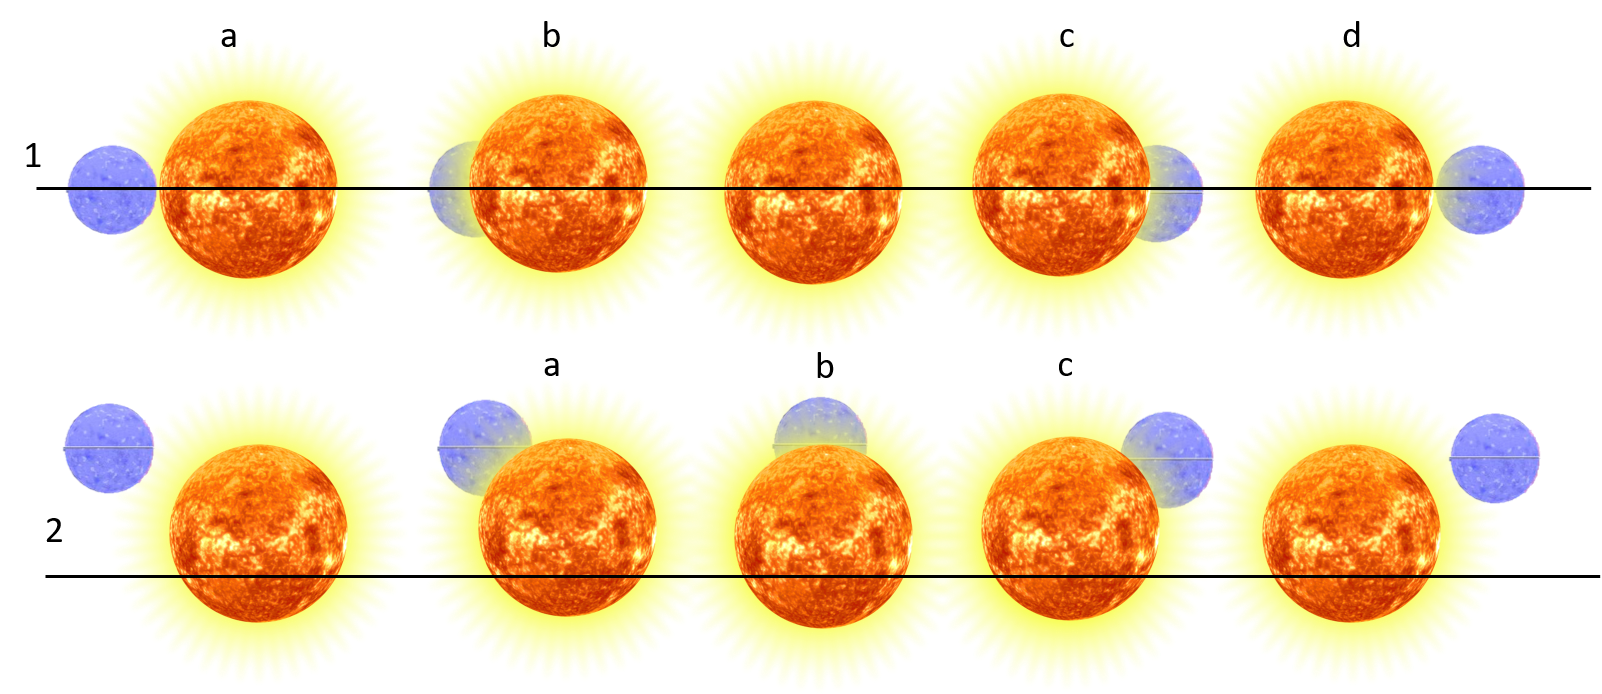
\includegraphics[width=1\linewidth]{Images/representacion_eclipse.png}
    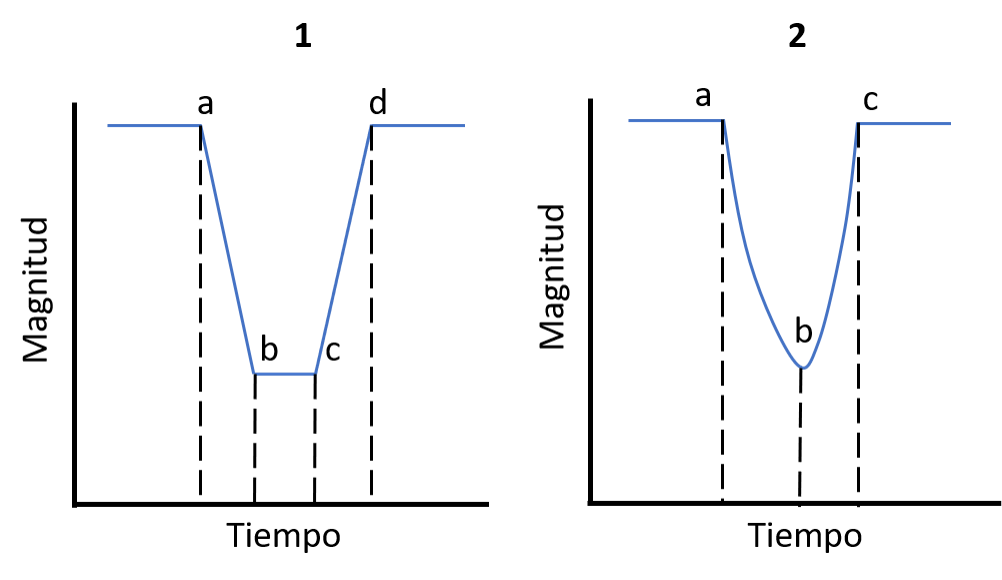
\includegraphics[width=0.62\linewidth]{Images/curva_luz_.png}
    \caption[Representación de un sistema binario eclipsante, con sus respectivas curvas de luz.]{Representación de un sistema binario eclipsante, con sus respectivas curvas de luz, sin tener en cuenta la geometría de algún sistema en específico, para diferentes variaciones de ángulo. En el 1) se tiene una inclinación $i = 90^{o}$, 1a es el primer contacto, 1b es eclipse parcial entrante y 1c es el parcial saliente, entre 1b y 1c es el eclipse total y 1d es el cuarto contacto. 2) la inclinación es menor a $90^{o}$.}
    \label{representacion_eclipse}
\end{figure}

\noindent Debido a las variaciones de luminosidad de la estrella principal durante el eclipse y descrita por su curva de luz, se puede hacer una buena estimación de la geometría del sistema. Esto nos permite deducir el ángulo de inclinación $i$ (medido como el ángulo entre el plano del observador y el eje de rotación de la estrella), como también excentricidad orbital. En la figura \ref{representacion_eclipse} se observa un ejemplo de la relación entre las asimetrías de la curva, con respecto a la geometría del sistema.



\noindent Existen tipos de sistemas estelares binarios eclipsantes característicos, donde una de sus componentes es una estrella gigante fría y la otra es una estrella en secuencia principal caliente. Estos sistemas se conocen como \textit{Sistemas $\zeta$ Aur} \citep{ake2015giants}. Si se tienen los espectros en orden temporal, es posible modelar los gradientes de densidad y temperatura en la cromósfera de la estrella gigante.

Siguiendo la figura \ref{representacion_eclipse}, en el primer contacto (1a) se tendrá una superposición de los espectros de la estrella gigante y la estrella compañera. A medida que las dos estrellas se acercan (1b) el flujo de la gigante cada vez se hace más débil por la presencia de la compañera, sobre todo en la banda azul. En ese momento se obtiene un espectro compuesto por las dos estrellas, no solo en superposición sino también con líneas de interacción cromosférica, debido a la interacción de la luz de la estrella compañera con la cromósfera de la estrella gigante. A medida que se oculta la estrella compañera, las líneas espectrales van cambiando su geometría. Finalmente en el eclipse total se obtiene solo el espectro de la estrella gigante, el cual se denomina \textit{espectro puro}. En el egreso de la estrella compañera (1c y 1d) ocurre un proceso análogo.

\subsection*{Sistema $\zeta$ Aurigae}\label{cap:zetaaur}

El sistema binario eclipsante $\zeta$ Aurigae fue descubierto en 1932 \citep{guthnick1934bevorstehende}. Este sistema se encuentra ubicado en la constelación de Auriga y sus eclipses estelares se pueden observar tanto con telescopios terrestres como espaciales, gracias a que durante el eclipse, la magnitud de $\zeta$ Aur A disminuye a +3,99 en la banda B. Otra de las características relevantes de este sistema, se pueden apreciar en la tabla \ref{tabla:parametroz_a}, con las respectivas citas que validan cada uno de los parámetros conocidos de las estrellas del sistema. Por otro lado, es relevante la geometría del eclipse, la cual puede ser observada en la figura \ref{fig:geometria} donde están los radios a escala de acuerdo a \citep{di1990angular}, para tener una mejor claridad de la relación de tamaños entre estrellas.

% En la tabla las unidades de radio es simplemente Rsun y masa es Msun. Si gustas puedes agregar los resultados de teff, log g y Fe/H de mi articulo en preparación.

\begin{table}[h]
\centering
\resizebox{16cm}{!}{
\begin{tabular}{|c|c|c|c|c|}
\hline
\textbf{Característica} & \textbf{Unidades}  & \textbf{$\zeta$ Aur A} & \textbf{$\zeta$ Aur B} & \textbf{Cita} \\ \hline
Subgrupo estelar        & -                  & \begin{tabular}[c]{@{}c@{}}Gigante\\ roja\end{tabular} & \begin{tabular}[c]{@{}c@{}}Secuencia\\ principal\end{tabular}    &   \cite{ake2015giants}            \\ \hline
Tipo espectral          & -                  & K5 II                  & B7 V                   &  \citep{shenavrin2011vizier}    \\ \hline
Periodo orbital         & días               & \multicolumn{2}{c|}{972.164 $\pm$ 0.041}        &  \cite{griffin2005spectroscopic}      \\ \hline
Periodo eclipsación     & días               & \multicolumn{2}{c|}{$\approx$ 36}               & \cite{griffin2005spectroscopic}    \\ \hline
Radios                  & $R_{\odot}$  & 166                    & 5.1                    &  \cite{schroder1997critical}             \\ \hline
Tasa masa               & $M_A/M_B$          & \multicolumn{2}{c|}{1.27 $\pm$ 0.6}             &  \cite{schroder1997critical}             \\ \hline
Masa                    & $M_{\odot}$  & 6.6$ \pm$ 0.7          & 5.2 $\pm$ 0.4         &  \cite{schroder1997critical}             \\ \hline
Luminosidad             & $log(L/L_{\odot})$ & 3.78                   & 3.07                   &  \cite{schroder1997critical}             \\ \hline
\begin{tabular}[c]{@{}c@{}}Temperatura\\ efectiva\end{tabular}     & $T_{eff}$ {[}K{]} & \begin{tabular}[c]{@{}c@{}}4057\\ 4150\end{tabular}           & 15000                  &  \begin{tabular}[c]{@{}c@{}}\cite{luck2014parameters}\\ \cite{schroder1997critical}\end{tabular}             \\ \hline
Gravedad superficial    & log(g)             &       0.54          &            -            &    \cite{luck2014parameters}           \\ \hline
Metalicidad             & Fe/H               &       -0.01           &            -            &  \cite{luck2014parameters}            \\ \hline
Velocidad radial        & $V_r$ {[}m/s{]}     & 11.32 $\pm$ 0.3        &         -           &  \cite{kps9}           \\ \hline
Paralaje*               & $\pi$                 & \multicolumn{2}{c|}{\begin{tabular}[c]{@{}c@{}}4.15 $\pm $0.29\\ 5.2872  $\pm$ 0.5353\end{tabular}}            &  \begin{tabular}[c]{@{}c@{}}\cite{van2007validation}\\ \cite{gaia2018vizier}\end{tabular}             \\ \hline
\end{tabular}
}
\caption{Parámetros y características de las estrellas que componen al sistema $\zeta$ Aurigae.}
\label{tabla:parametroz_a}
\end{table}

\begin{figure}[H]
    \centering
    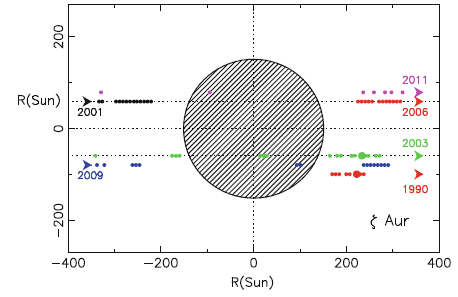
\includegraphics[width=0.65\linewidth]{Images/Geometria_eclipse.PNG}
    \caption[Geometría a escala del sistema $\zeta$ Aur.]{Geometría a escala del sistema $\zeta$ Aur, que indica el seguimiento de seis eclipses. Las trayectorias modeladas se han desplazado verticalmente para mayor claridad, pero todas deberían estar a lo largo de la misma. Datos de 1990: espectros fotográficos del Calar Alto Observatory; y otros: espectros CCD del DAO.}
    \label{fig:geometria}
\end{figure}

\noindent Los valores de de radios, luminosidades y demás características de las estrellas, como se observa en el cuadro \ref{tabla:parametroz_a}, se derivan de una combinación de fotometría y espectroscopia, con esto se puede hacer coincidir sus posiciones en el diagrama H – R. También se pueden reconstruir con las trayectorias evolutivas calculadas para sus masas correspondientes \citep{schroder1997critical}, lo que proporciona una verificación muy valiosa de los parámetros y supuestos que la teoría de la evolución ha adoptado.

\noindent En la actualidad, los sistemas binarios tienen un potencial único como trazadores de la evolución estelar, permitiendo extrapolar características a estrellas individuales. Esto se basa en la condición de que la evolución de un miembro de un sistema binario no se ve afectada por su unión gravitacional con otra estrella, como se indica en \citep{schroder1997critical}. Los modelos de cromósferas que se producen al analizar los eclipses atmosféricos de los sistemas Aur son representativos con respecto a otras gigantes. Con el estudio de líneas como las líneas H y K de Ca II y los cambios de ionización se pueden conocer, si a pesar de enfoques diferentes relacionados con los vientos exteriores y cromósferas hay compatibilidades entre binarios e individuales.




\section{Espectroscopia Estelar}\label{espectroscopia}

\noindent Desde la antigüedad, nuestros antepasados se han preguntado por la composición de las estrellas que podemos observar en el firmamento. Gracias a la luz que nos llega de las mismas, actualmente podemos conocer la respuesta a ésta y muchas más incógnitas planteadas años atrás. La espectroscopia es una de las herramientas más útiles en el análisis de objetos astronómicos.
\vspace{2mm}

\noindent Isaac Newton fue el primero en usar la palabra \textit{espectro} refiriéndose a los colores en que se descompone la luz blanca al pasar por un prisma. Posteriormente, el astrónomo, óptico y físico alemán Joseph von Fraunhofer, usó un espectroscopio para descomponer la luz proveniente del Sol y además de ver un continuo de colores, observó la presencia de líneas oscuras, como se observa en la figura (\ref{espectro_frauhofer}). Fraunhofer no pudo explicar este comportamiento \citep{von1823denkschriften}. En el siglo XIX, Gustav Robert Kirchhoff y Robert Wilhelm Bunsen observaron que cuando los elementos químicos alcanzan ciertas temperaturas, emiten luz en longitudes de onda específicas, es decir, cada elemento tiene un espectro de líneas único y característico.

\begin{figure}[h]
    \centering
    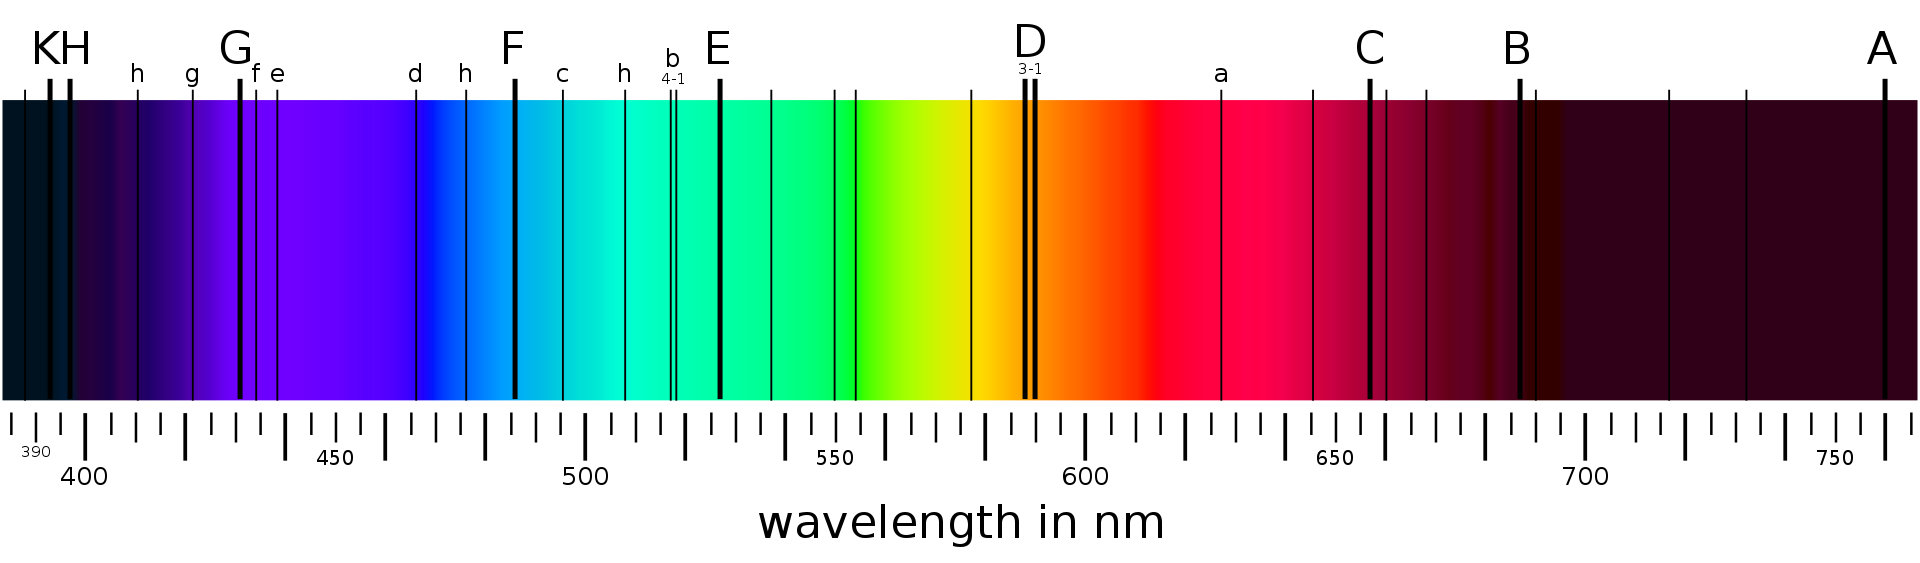
\includegraphics[width=1\linewidth]{Images/espectro_fraunhofer.png}
    \caption{Representación gráfica de las líneas de Fraunhofer. Dominio público, Wikimedia Commons.}
    \label{espectro_frauhofer}
\end{figure}

\noindent En 1886, el físico y astrónomo estadounidense Edward Pickering en conjunto con un equipo de 13 mujeres conocidas como \textit{las calculadoras de Harvard}, retomaron un trabajo hecho por el astrónomo Angelo Secchi en 1874, el cual propuso una clasificación para las líneas espectrales. El equipo contó y clasificó aproximadamente 225.300 estrellas, registrándolas en el \textit{Henry Draper Catalogue} \citep{gray2009stellar}. Además propusieron un primer sistema de clasificación espectral que posteriormente se convirtió en el conocido sistema Morgan-Keenan (``OBAFGKM'' con divisiones de 0 a 9), el cual está directamente relacionado con la temperatura. Las primeras estrellas se conocen como \textit{tipo temprano} y suelen ser azules y calientes, mientras que las últimas se conocen como \textit{tipo tardío} y suelen ser rojas y frías.
\vspace{2mm}

\noindent Posteriormente, los astrónomos Ejnar Hertzsprung y Henry Russell, propusieron el célebre diagrama Hertzsprung-Russell o \textit{diagrama H-R}. El cual registra: magnitud absoluta o luminosidad en el eje vertical (con el aumento de brillo hacía arriba) y el tipo espectral o índice de color en el eje horizontal (con la temperatura aumentando hacía la izquierda). Las estrellas se pueden dividir en subgrupos: secuencia principal (MS), Gigantes (G), Supergigantes (SG) y Enanas (D).

\noindent Teniendo en cuenta todas las propiedades mencionadas anteriormente, se puede conocer la evolución estelar a partir de la secuencia de cambios dinámicos de las estrellas. Para entender los espectros estelares es necesario conocer la estructura estelar de dónde viene la luz que analizamos, y cómo en su interior se forman esos espectros que posteriormente se van a analizar.


\subsection{Ecuaciones de Boltzman y Saha}

% De la wikipedia:  la ecuación de Boltzmann describe el comportamiento estadístico de un sistema termodinámico fuera del equilibrio termodinámico. Ese primer párrafo introductorio me parece algo enredado y no da una introduccion a las ecuaciones. ni explicas el por qué son necesarias.

\noindent Es muy importante tener en cuenta cómo medir las abundancias químicas en las atmósferas estelares, tanto para elementos neutros como ionizados, para esto se implementa la herramienta de espectroscopia (\textit{este tema es explicado de manera más profunda en la sección \ref{sec:para_est}}).  Teóricamente se implementan las ecuaciones de Boltzmann \ref{eq:boltzmann} y de Saha \ref{saha} para cada uno de los elementos, respectivamente.
\vspace{2mm}

\noindent Para describir la ecuación de Boltzmann de un sistema en equilibrio termodinámico, es necesario conocer la función de distribución de velocidades de Maxwell-Boltzmann, como se ve en la ecuación (\ref{eq:boltzmann}). Esta distribución describe la fracción de partículas por unidad de volumen, $n_v = \partial n / \partial v$ que están en un rango de velocidades $v + dv$. Donde $n$ se refiere a la densidad total, $m$ es la masa del electrón, $T$ la temperatura de excitación y $k$ la constante de Boltzmann

\begin{equation}
n_{v} d v=n\left(\frac{m}{2 \pi k T}\right)^{3 / 2} e^{-m v^{2} / 2 k T} 4 \pi v^{2} d v.
\label{eq:boltzmann}
\end{equation}

\noindent Ahora, los átomos de un gas, no solo tienen una velocidad caracterizada con la ecuación (\ref{eq:boltzmann}), sino  que también ganan y pierden energía a medida que interactúan con los fotones. Teniendo en cuenta estas dos características, es posible obtener una distribución de electrones en el átomo. Ésta se rige por un resultado fundamental de la mecánica estadística \citep{carroll2017introduction}, es decir, es menos probable que los orbitales de mayor energía estén ocupados por electrones. Entonces la relación de probabilidades de que un electrón esté en un estado $a$ o uno $b$ está dado en la ecuación \ref{ec:prob}, donde el término $e^{-E_{b} / k T}$ se conoce como factor de Boltzmann

\begin{equation}
\frac{P_b}{P_a}=\frac{e^{-E_{b} / k T}}{e^{-E_{a} / k T}}=e^{-\left(E_{b}-E_{a}\right) / k T}.
\label{ec:prob}
\end{equation}

\noindent Es necesario tener en cuenta los \textit{estados degenerados}, es decir, aquellos  en los cuales a pesar de que los números cuánticos son diferentes, las energías son iguales. Para estos casos cada estado degenerado debe ser que contado independientemente. Por lo tanto, ahora es necesario tener en cuenta pesos estadísticos $g_i$, los cuales están relacionados directamente con las energías y no con los números cuánticos, de este modo, tener en cuenta todos los estados posibles.

\noindent Esto conlleva a la ecuación de Bolztmann (\ref{eq:Boltzmann_real}), que es la razón de la cantidad de átomos de un elemento, con diferentes estados de excitación. Donde $N_b$ es el número de átomos con energía $E_b$ y $N_a$ los átomos con energía $E_a$

\begin{equation}
\frac{N_{b}}{N_{a}}=\frac{g_{b} e^{-E_{b} / k T}}{g_{a} e^{-E_{a} / k T}}=\frac{g_{b}}{g_{a}} e^{-\left(E_{b}-E_{a}\right) / kT}.
\label{eq:Boltzmann_real}
\end{equation}


\noindent Por otro lado, se pueden tener en cuenta átomos ionizados, es decir, cuando se desliga un electrón del estado base con una energía de  ionización $\chi_i$. Esto es, llevándolo de la etapa de ionización $i$ a $i+1$, la ecuación de Boltzmann se reescribe como la ecuación \eqref{saha}. Ésta es conocida como \textit{ecuación de Saha}, donde $Z(T)$ es la función de partición dependiente de la temperatura, $N_i^{ion}$ es un modelo de densidad de iones en función de la altura atmosférica y $T_{exc}$ es la temperatura de excitación

\begin{equation}
A_{i} = \frac{\pi e^{2}}{m_{e} c^{2}} \frac{\lambda c}{v \sqrt{\pi}} g f \frac{N_{i}^{ion}}{Z(T)} e^{-E_{i} / k T_{exc}}.
\label{saha}
\end{equation}

\subsection{Formación de líneas estelares}

Las líneas de absorción se crean cuando un átomo absorbe un fotón con la energía requerida para que un electrón realice una transición de un orbital inferior a uno superior. Las líneas de emisión se forman en el proceso inverso, cuando un electrón hace una transición descendente y se libera un fotón. Matemáticamente esto se puede escribir como en la ecuación (\ref{eq:energia_foton}). Además, la longitud de onda del fotón depende de las energías de los orbitales atómicos involucrados en estas transiciones, las cuales también se pueden distinguir aplicando las ecuaciones de Boltzmann (\ref{eq:Boltzmann_real}) y Saha (\ref{saha}). Por lo que cada línea espectral corresponde a una transición específica de un átomo en concreto. Las líneas nos permiten identificar los átomos presentes en la atmósfera de la estrella, y por tanto su composición química

\begin{equation}
    E_{\gamma} = n(E_f - E_i) = h \nu = hc/\lambda.
    \label{eq:energia_foton}
\end{equation}

\noindent Las transiciones de electrones de un orbital a otro, también tienen una fuerte relevancia en la física atómica, ya que hay parámetros físicos y estadísticos que condicionan las probabilidades de que se de una transición o no. Uno de los repositorios que contiene información al respecto es \textit{Vienna Atomic Line Data Base (VALD)} \citep{piskunov1995vald}. Este repositorio contiene la compilación de datos teóricos y experimentales relevantes para las transiciones atómicas que contribuyan significativamente a la absorción en los espectros estelares.


\noindent Las diferencias entre los espectros de dos estrellas se deben tanto a sus diferentes temperaturas, como a su composición química. Los detalles de la formación de líneas espectrales pueden ser complejos. Puesto que la emisión o absorción puede deberse a la transición de un electrón de cualquier átomo presente en la atmósfera estelar, en cualquiera de las etapas de ionización.


\noindent Para descubrir las bases físicas de la clasificación estelar se debe conocer la formación de las líneas de absorción y emisión. También se debe conocer con claridad, la probabilidad de encontrar un electrón en un orbital para que este haga una transición y además conocer las etapas de ionización los átomos. Para esto, se cuenta con la rama de la física estadística, donde se analiza la \textit{opacidad}, la cual es una característica que tiene en cuenta cuatro fuentes primarias para eliminar fotones estelares de un haz. Estas fuentes implican cambios de estado cuántico de electrones y los términos ligado y libre, que hacen referencia a si un electrón está unido al átomo o se trata de un ion en estado final o inicial.

\begin{itemize}
    \item[1.] \textbf{Interacción ligado-ligado} se producen cuando un electrón de un átomo realiza una transición de un orbital a otro y permanece ligado al átomo. De forma ascendente cuando gana energía por la apropiada absorción de un fotón, estás transiciones son responsables de líneas de absorción. En el proceso inverso, con transiciones descendentes, por volver al estado inicial o de menor energía, se emite un fotón y el resultado de esta secuencia es absorción-emisión. Si no vuelve a su estado inicial es una absorción pura. Si, mientras está en un estado excitado, tiene una colisión con una partícula vecina, lo que se convierte en parte de la energía térmica del gas, y genera degradación de la energía media de los fotones. No existe una única ecuación que tenga en cuenta todas estas posibles contribuciones.
    
    \item[2.] \textbf{Interacción ligado-libre}, también conocida como \textit{fotoionización}, ocurre cuando un fotón incidente tiene energía mayor a la energía de ionización, es decir, la suficiente para ionizar un átomo y arrancar un electrón. Cualquier fotón de $\lambda \leq hc/\chi_i$, donde $\chi_i$ es la energía de ionización del i-ésimo orbital. Puede ser absorbido y esa energía se usa para arrancar un electrón del átomo. Esta absorción es continua, porque no se necesita una energía específica y puede producir una disminución de energía en el continuo espectral. 
    
    El proceso inverso sucede cuando el electrón libre se recombina con un ion emitiendo fotones en direcciones aleatorias y contribuye a reducir la energía promedio de fotones en el campo de radiación.
    
    \item[3.] \textbf{Interacción libre-libre} es un proceso de dispersión, cuando un electrón libre cerca de un ion, absorbe un fotón, lo que hace que aumente la velocidad del electrón. En este proceso, el ion cercano es necesario para conservar tanto la energía como el impulso. También puede pasar que al pasar cerca a un ion el electrón pierde energía al emitir un fotón, lo que hace que el electrón se desacelere, este proceso de emisión libre se conoce como \textit{bremsstrahlung}, que significa ``radiación de frenado''.
    
    Debido a estas dispersiones, los átomos en estado excitado que son inestables, por lo que luego el átomo se desexcita espontáneamente emitiendo de nuevo el fotón. Ese fotón a su vez lo vuelve a absorber otro átomo, y es vuelto a emitir, y así sucesivamente. Los fotones quedan de esta forma atrapados en la atmósfera y lo vemos evidenciado en las líneas de absorción.
    
    Como la fotosfera sigue aportando luz en todas las longitudes de onda, llegaría un momento en que los electrones capturados por una transición serían tantos que mantendrían todos los átomos excitados, como si estos fuesen estables. Los nuevos fotones emitidos por la fotosfera en esa longitud de onda ya no serían absorbidos, pues no tendríamos electrones en el nivel de energía bajo del inicio de la transición. Los fotones saldrían de la atmósfera, formarían parte del espectro, y la línea desaparecería. A este fenómeno se denomina \textit{saturación de la línea}.

    \item[4.] \textbf{Dispersión de electrones} es cuando un electrón dispersa un fotón a través del proceso de \textit{dispersión de Thomson}, es decir, el electrón oscila en el campo electromagnético del fotón. Sin embargo, como el electrón es pequeño, resulta en una pequeña región transversal, lo que significa que la dispersión electrónica es más efectiva cuando la densidad de electrones es muy alta, lo que requiere también una alta temperatura.
    \end{itemize}
    


%%%%%%%%%%%%%%%%%%%%%%%%%%%%%%%
%%%%%%%%%   Section   %%%%%%%%%
%%%%%%%%%%%%%%%%%%%%%%%%%%%%%%%
\section{Atmósfera estelar: Fotósfera}\label{sec:atm_est}

%De estructura estelar solar, ya que no todas las estrellas tienen esa misma estructura. ver carrol

El modelo más simple de estructura estelar son capas esféricas superpuestas, dentro de las cuales se encuentra el núcleo estelar, la zona radiativa, zona convectiva y atmósfera estelar, esta estructura se observa en la figura \ref{fig:estruct_est}. La atmósfera en estrellas desde la \textit{O} hasta las \textit{K0} están compuestas por fotósfera, cromósfera y corona. Para las estrellas superiores a las \textit{K2} se tiene fotósfera, cromósfera y viento solar frío. En ambos casos, la cromósfera se comporta como una zona de transición.

\begin{figure}[h]
    \centering
    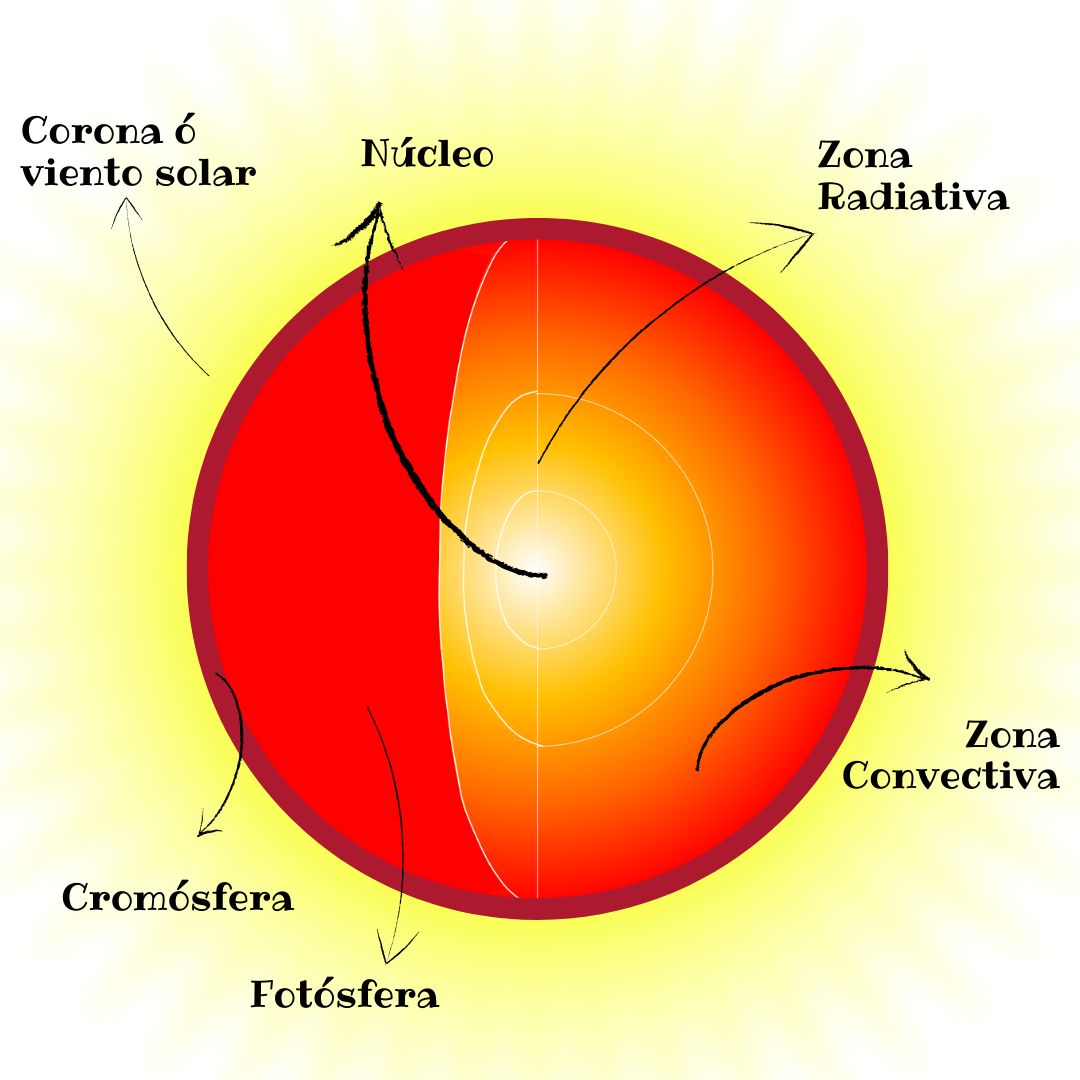
\includegraphics[width=0.7\linewidth]{Images/estructura_sol.png}
    \caption{Esquema de la estructura de estrellas, las \textit{tipo solar} tienen corona y las \textit{no solar} vientos solares. El esquema no está a escala.}
    \label{fig:estruct_est}
\end{figure}

\noindent La fotósfera está compuesta principalmente de gas y una pequeña porción en forma de plasma o gas ionizado, el cual es opaco a la radiación. Por lo tanto, no es fácil conocer el interior de las estrellas. Sin embargo, el gas atómico o molecular da paso a la luz, lo cual se conoce como continuo espectral y puede ser detectado por los telescopios. Esto forma lo que conocemos como espectro estelar, así que para interpretarlo, es necesario describir cómo viaja la luz a través del gas estelar.

\noindent Como primera aproximación, la energía por longitud de onda de una estrella puede modelarse como un radiador perfecto mediante la ley de Planck (ecuación \ref{ley_planck}). Donde $h = \num{6,063e-34}\,[J]$, conocida como la constante de Planck, $k = \num{1,38e-23}$ $[JK^{-1}]$ es la constante de Boltzman, $c= \num{3e8}\,[m/s]$ es la velocidad de la luz en el vacío y $T$ la temperatura

\begin{equation}
    B(\lambda,T) = \frac{2h c^2}{\lambda^5} \frac{1}{e^{h c/k\lambda T}-1}.
    \label{ley_planck}
\end{equation}

\noindent Para conocer el pico máximo de emisión de energía, es necesario derivar la ecuación \ref{ley_planck}, obteniendo la longitud de onda donde ocurre esta emisión, a esto se le conoce como \textit{ley de desplazamiento de Wien}, (ecuación \ref{wien}). Donde $A = $ 0.0028976 [m$\cdot$ K] se denomina la constante de Wien y $\lambda_{max}$ es la longitud de onda de máxima emisión

\begin{equation}
    \lambda_{max} =  \frac{A}{T}.
    \label{wien}
\end{equation}

\noindent Al integrar la ecuación \ref{ley_planck}, asumiendo que una estrella irradia isotrópicamente, se obtiene la energía radiada por unidad de tiempo y unidad de área conocida como \textit{ecuación de Stefan-Boltzmann} (ecuación \ref{stefan-boltzman}), donde $\sigma = \num{5,67 e-8}$ [W/m$^2$K$^4$] se conoce como constante de Stefan-Boltzmann.
\vspace{2mm}

\begin{equation}
    F = 4 \pi \int B(\lambda)  d\lambda = \sigma T^4
    \label{stefan-boltzman}
\end{equation}

\noindent En la figura  (\ref{fig:lineblanketing}) se observa que modelar las estrellas como un radiador perfecto que sigue la ley de Planck, se usa más por su sencillez que por su exactitud, ya que las líneas de emisión y absorción de los espectros afectan el continuo en ciertas longitudes de onda. En el caso de estrellas gigantes, que se caracterizan por su alta cantidad de metales, los espectros poseen gran cantidad de líneas de absorción y en estos casos, este continuo se ve más afectado. Esta alta absorción, hace que se reduzca la intensidad del continuo y en ocasiones no se observen las líneas individuales. A este fenómeno se le conoce como \textit{blanketing effect} o \textit{line blanketing}, con un efecto bastante pronunciado en las regiones azules del espectro.

\begin{figure}[H]
    \centering
    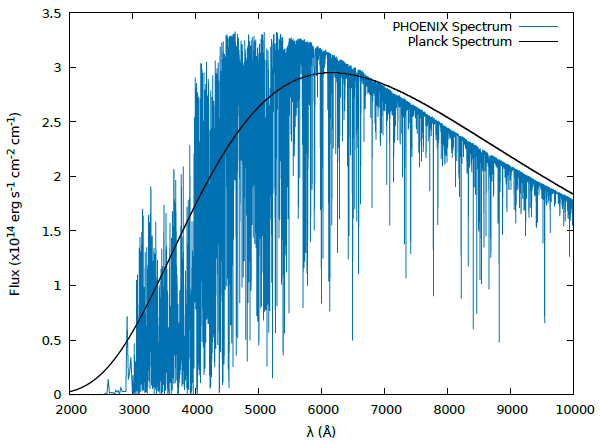
\includegraphics[width=0.85\linewidth]{Images/lineblanck.PNG}
    \caption[Comparación entre un modelo de espectro estelar a $T = 4700 K$ generado con el código PHOENIX, y una curva de cuerpo negro a la misma temperatura.]{Comparación entre un modelo de espectro estelar a $T = 4700 K$ generado con el código PHOENIX, y una curva de cuerpo negro a la misma temperatura. La resolución del espectro se ha disminuido en un factor de 200. \textit{Tomado de \citep{Faiber2019master}}.}
    \label{fig:lineblanketing}
\end{figure}



\begin{comment}
un caso de estas líneas que no son producidas en la fotósfera como normalmente es esperado, son las líneas H y K, debido a la fenómenos físicos como la gravedad superficial $log(g)$ o la densidad de masa columnar $\sigma_{cm}$.
\end{comment}



\begin{comment}
\noindent Además, como las atmósferas no están compuestas de gas solamente de Hidrógeno sino que hay combinaciones e impactos que producen átomos más pesados como el Helio, pero en menor cantidad, normalmente 10 átomos H por cada 1 de He. Por lo que la presencia de otros átomos ionizados proporciona más electrones con los que los iones de Hidrógeno pueden volverse a combinar. Así que las temperaturas se van elevando para dar paso a este tipo de fenómenos.
\end{comment}




\subsection*{Espectros de la fotósfera del  sistema $\zeta$ Aur}\label{ssec:lineasfoto}

Unas de las líneas espectrales de la estrella gigante del sistema $\zeta$ Aur, que además es fácil de reconocer, debido a su ancho, son las líneas de Fraunhofer de Calcio doblemente ionizado (Ca II): H (396.847 nm) $\&$ K (393.368 nm). Estas líneas se pueden observar en la figura \ref{fig:lineafotos}, respectivamente.

\begin{figure}[h]
    \centering
    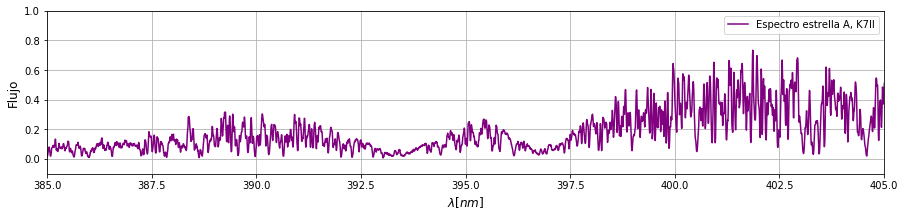
\includegraphics[width=1\linewidth]{Images/Lineas_fotosfera.png}
    \caption{Espectro puro del último eclipse (2019) de la estrella A del sistema $\zeta$ Aurigae, tipo K7II.}
    \label{fig:lineafotos}
\end{figure}


Estas dos líneas de absorción características son generadas en la fotosfera y de acuerdo a que la temperatura en esta región de la atmósfera no es tan alta se puede asumir equilibrio térmico local. Éstas se generan porque el átomo gana energía por el impacto de un fotón haciendo que haya una transición a un nivel superior de energía y que al bajar de manera espontánea a su estado fundamental se emita un fotón de la misma naturaleza que el absorbido. 


En esta zona de la fotosfera, según las ecuaciones de Saha y Boltzmann no se obtienen líneas de emisión debido a las bajas temperaturas y altas densidades, no obstante estas pueden generarse en la cromósfera.

%%%%%%%%%%%%%%%%%%%%%%%%%%%%%%%
%%%%%%%%%   Section   %%%%%%%%%
%%%%%%%%%%%%%%%%%%%%%%%%%%%%%%%

\section{Atmósfera estelar: Cromósfera}

La cromósfera es la zona de transición entre la fotósfera y la corona o el viento estelar, de acuerdo al tipo de estrella. La definición exacta de cromósfera en la actualidad no está perfectamente detallada o delimitada en las alturas de la atmósfera. Inicialmente se ha determinado como una capa atmosférica en la que hay una cantidad mensurable de calentamiento local, además del transporte de calor radiactivo y convectivo que se tiene en la fotósfera. 

Los límites de la cromosfera se pueden definir por el signo del gradiente térmico de la atmósfera estelar\citep{linsky2017stellar}. Las fuentes de calor no radiantes son débiles como para modificar significativamente el equilibrio de la entrada de energía radiante y convectiva con respecto a las pérdidas radiantes en el espacio. Debido a que las densidades son relativamente grandes en la parte superior fotosfera, el enfriamiento radiativo es muy eficiente, y la tasa de calentamiento no radiativo es mucho mayor que en las capas de menor densidad de la cromosfera. A su vez, la disminución de densidad a cierta altura atmosférica, hace que la combinación del calentamiento no radiactivo y la disminución del enfriamiento radiactivo, genere un aumento de la temperatura con la altura. Como vemos entonces unas de las características más relevantes es el comportamiento de la temperatura y la densidad, las cuales van inversamente proporcionales. En la figura (\ref{perfil:densidad-temp}) se observan las variaciones en estas propiedades a través de la atmósfera estelar.

\begin{figure}[h]
    \centering
    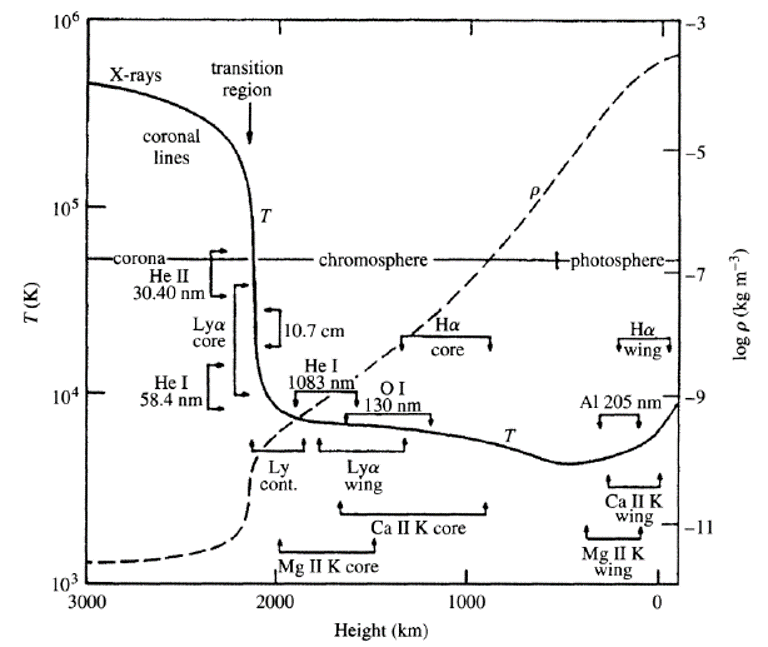
\includegraphics[width=0.8\linewidth]{Images/perfil_Densidad-temperatura.png}
    \caption[Perfiles de temperatura y densidad de masa en relación con la altura de la atmósfera solar.]{Perfiles de temperatura (línea solida) y densidad de masa (línea punteada) en relación con la altura de la atmósfera solar. Se muestra también las zonas de los perfiles donde se forman algunas líneas espectrales. Fuente \citep{vernazza1973structure}.}
    \label{perfil:densidad-temp}
\end{figure}

Al variar la altura atmosférica o la profundidad óptica las líneas de absorción y emisión, cada capa se pueden relacionar con diferentes mecanismos físicos que están sucediendo dentro de la atmósfera, como la radiación y convección. Sin embargo, aún no es factible modelar por completo la atmósfera estelar en toda su complejidad. Los modelos de atmósferas actuales son buenas aproximaciones para ciertas regiones, por lo tanto, siguen siendo un tema relevante en la actualidad. Hay mecanismos como los mostrados en \citep{chavez2013new} y \citep{ayres2019stellar}, donde los campos magnéticos son cada vez más importantes para explicar altas temperaturas a las que puede llegar la cromósfera y algunas de sus complejidades.

\begin{comment}


Normalmente no es tan sencillo diferenciar qué líneas son originadas en la fotósfera y cuáles de ellas se originan en la cromósfera, pero de acuerdo a las temperaturas y los datos que se pueden obtener con el tratamiento de las líneas se podría saber las diferencias. Además a diferencia de las líneas fotosféricas que pueden tener un amortiguamiento notable, las líneas de la cromósfera suelen caracterizarse por ser más \textit{fuertes}.


Con los sistema $\zeta$ Aur, se puede hacer un tratamiento adicional para obtener las líneas cromósfericas de la estrella gigante. Esto se logra con una sustracción de espectral entre un espectro combinado del eclipse parcial y el espectro puro de la estrella gigante en el eclipse total. La luz de la estrella en secuencia principal se encuentra por detrás de la atmósfera de la estrella gigante, con respecto a nuestra línea de visión, por lo que la cromósfera absorbe su luz. 
\end{comment}

\subsection*{Espectros de la cromósfera del  sistema $\zeta$ Aur}

\noindent Como se nombraba en el espectro de la fotósfera, una de las líneas más reconocidas de la estrella gigante del sistema $\zeta$ Aur es la línea H de Ca II (396.847 nm). La formación de esta línea es muy particular ya que como se observa en la figura (\ref{fig:lineaCaii}) está compuesta por dos picos de emisión $K_2$ que se diferenciaran como pico azul, al derecho $K_{2B}$ y pico rojo $K_{2R}$, también se ven dos picos de absorción pura $K_1$ que al igual que en los picos de emisión se llaman $K_{1B}$ y $K_{1R}$ y un último pico en medio que también es de absorción $K_3$.

\begin{figure}[h]
    \centering
    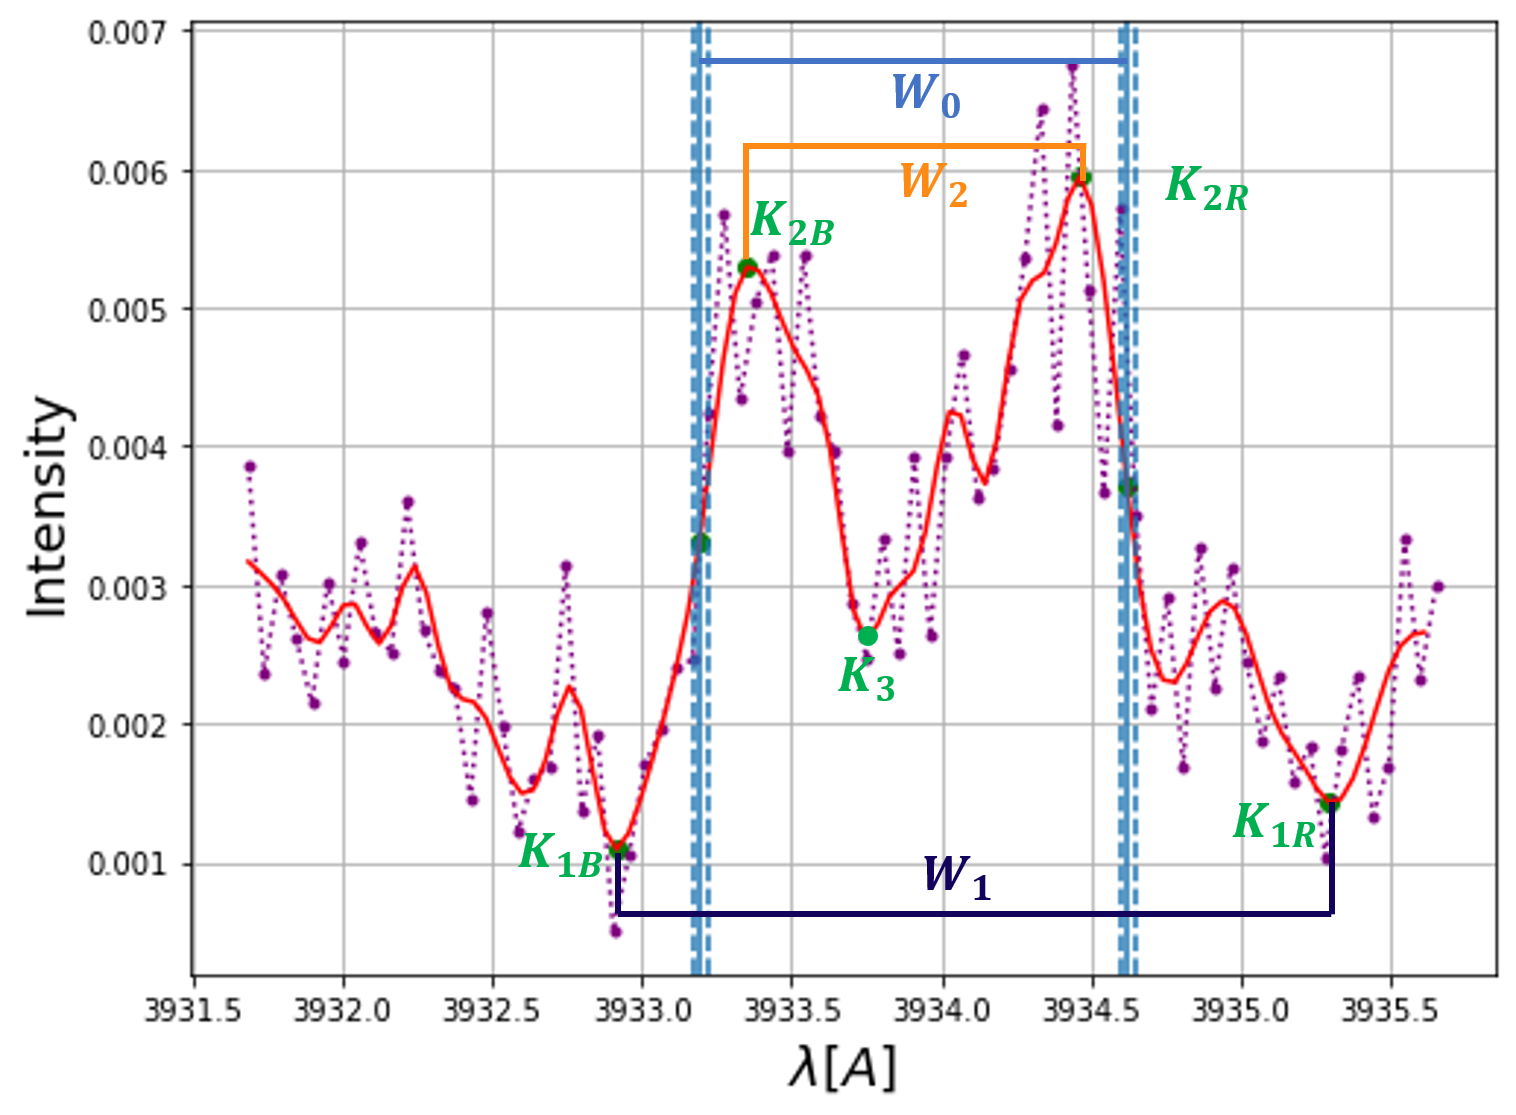
\includegraphics[width=0.8\linewidth]{Images/lineaCaii.png}
    \caption{Datos y ajuste por splines de la línea H de Ca II de la estrella gigante durante la totalidad del eclipse 2019.}
    \label{fig:lineaCaii}
\end{figure}

\noindent La formación de los picos de absorción $K_1$ se dan en la fotósfera como se describió en la sección \ref{ssec:lineasfoto}. Los picos de emisión $K_2$ son generados en la cromósfera baja según las ecuaciones de Saha y Boltzmann ya que en esta porción se sigue cumpliendo el equilibrio termodinámico. En este caso para que el átomo emita un fotón no es necesaria la absorción de un fotón, sino que el átomo suba de nivel debido a energía térmica ya que las temperaturas en esta zona son más elevadas, cumpliendo la distribución de velocidades de Maxwell. Por último el pico $K_3$ se conoce como \textit{autoabsorción}, debido a que no es una absorción pura como en el caso de $K_1$, este pico que se da en la cromósfera alta, donde ya no se cumple el equilibrio termodinámico, por ende tampoco se aplican las ecuaciones de Boltzmann y Saha. En esta porción de la atmósfera se tienen átomos con electrones tan excitados y con una densidad electrónica tan baja que cuando hay interacción de fotones lo que se obtiene es un fenómeno de \textit{scattering} o dispersión.

\noindent Por otro lado, también se observa en la figura (\ref{fig:lineaCaii}) que esta línea no es necesariamente simétrica, pero estas formas aún hacen parte de estudios físicos ya que es bastante complicado de relacionar. Además el hecho de que el pico $K_3$ esté desplazado al azul, también se asocia a fuerte presencia de viento estelar o debido a simetrías no esféricas en el material cromosférico, según \citep{linsky1980stellar}.

Lo cual resulta un análisis muy importante y que nos puede brindar mucha información sobre la atmósfera de la estrella, pero esto solo nos da información a una altura específica. Si se analizan otros elementos, y en diferentes fechas del eclipse es posible obtener información de la atmósfera a diferentes altitudes.


Además para este caso, de un sistema binario eclipsante, tenemos el espectro de la componente $\zeta$ Aur A (estrella gigante) que se puede observar durante el eclipse total. Pero también tenemos el espectro combinado de las dos estrellas y las líneas de absorción cromosférica superpuestas debido a que la luz de la estrella $\zeta$ Aur B (secuencia principal) debe pasar por la cromósfera durante el eclipse parcial. Estos espectros se pueden observar en la figura \ref{fig:espectro_zaur}. Donde además se hizo la sustracción para obtener solo los espectros de las líneas que la cromósfera de $\zeta$ Aur A absorbe de $\zeta$ Aur B.


\begin{figure}[h]
    \centering
    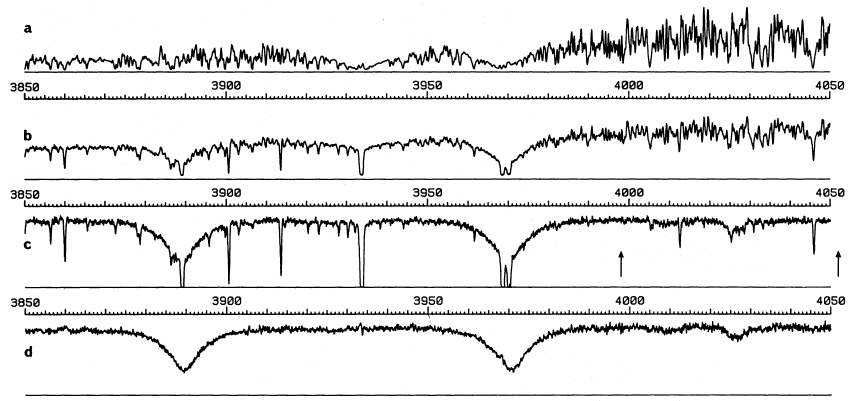
\includegraphics[width=1\linewidth]{Images/espectro_zeta_aur.PNG}
    \caption[Espectros en la banda B entre 3850 - 4050 \r{A} del eclipse de $\zeta$ Aurigae de 1987.]{Espectros en la banda B entre 3850 - 4050 \r{A} a) Espectro puro de la componente $\zeta Aur A$ durante el eclipse total b) Espectro compuesto del sistema binario durante el eclipse parcial c) Sustracción del espectro de la componente $\zeta$ Aur B y la superposición de las líneas de absorción cromosférica d) Espectro puro de la componente $\zeta$ Aur B \textit{Tomado de \citep{kps9}}.}
    \label{fig:espectro_zaur}
\end{figure}


Con la figura \ref{fig:espectro_zaur} se representa paso a paso el proceso de obtención de las líneas cromósfericas a partir de los espectros combinados para cada fecha durante el eclipse parcial, lo cual se implementa en este proyecto de tesis y se explica con mayor detalle en la sección \ref{sec:sustraccion}.
%%%%%%%%%%%%%%%%%%%%%%%%%%%%%%%
%%%%%%%%%   Section   %%%%%%%%%
%%%%%%%%%%%%%%%%%%%%%%%%%%%%%%%




\section{Densidad de Masa columnar}\label{sec:densidad_masa}
La densidad de masa columnar o densidad columnar es la cantidad de materia que recorre un fotón, pasando por la atmósfera en la línea de visión del observador \citep{carroll2017introduction}. Matemáticamente se escribe como la integral de la densidad de masa volumétrica $\rho (z)$, la cual es radial y puede tener la forma de ley de potencias. También se describe como la cantidad de átomos de una misma especie en un área infinitesimal de atmósfera dependiente de la altura atmosférica a lo largo de la columna $dz$ como se observa en la ecuación \ref{ec:denscolumnar}. Además en la figura \ref{fig:rep_dens_masa} se puede ver una representación gráfica como referencia a esta magnitud, teniendo en cuenta las variaciones de temperatura y de densidad en la atmósfera

\begin{equation}
    N = \int_a^b n (z) dz.
    \label{ec:denscolumnar}
\end{equation}

\noindent Gracias a la espectroscopía, es posible conocer la densidad de masa columnar ($N$), y es necesario ya que es una magnitud que afecta el ensanchamiento de las líneas espectrales. Con $N$ se puede hacer un modelado estelar cromosférico, ya que si se obtiene $N$ a partir de líneas de absorción pura que se forman en esta área de la atmósfera y se pueden obtener buenos modelos empíricos a alturas intermedias. Normalmente esto se hacen con líneas fuertes, pero no saturadas, los elementos empleados, varían según el tipo de estrella que se analice, para el caso de estrellas gigantes, se usan líneas de Fe I, Ti II e H.

\begin{figure}[h]
    \centering
    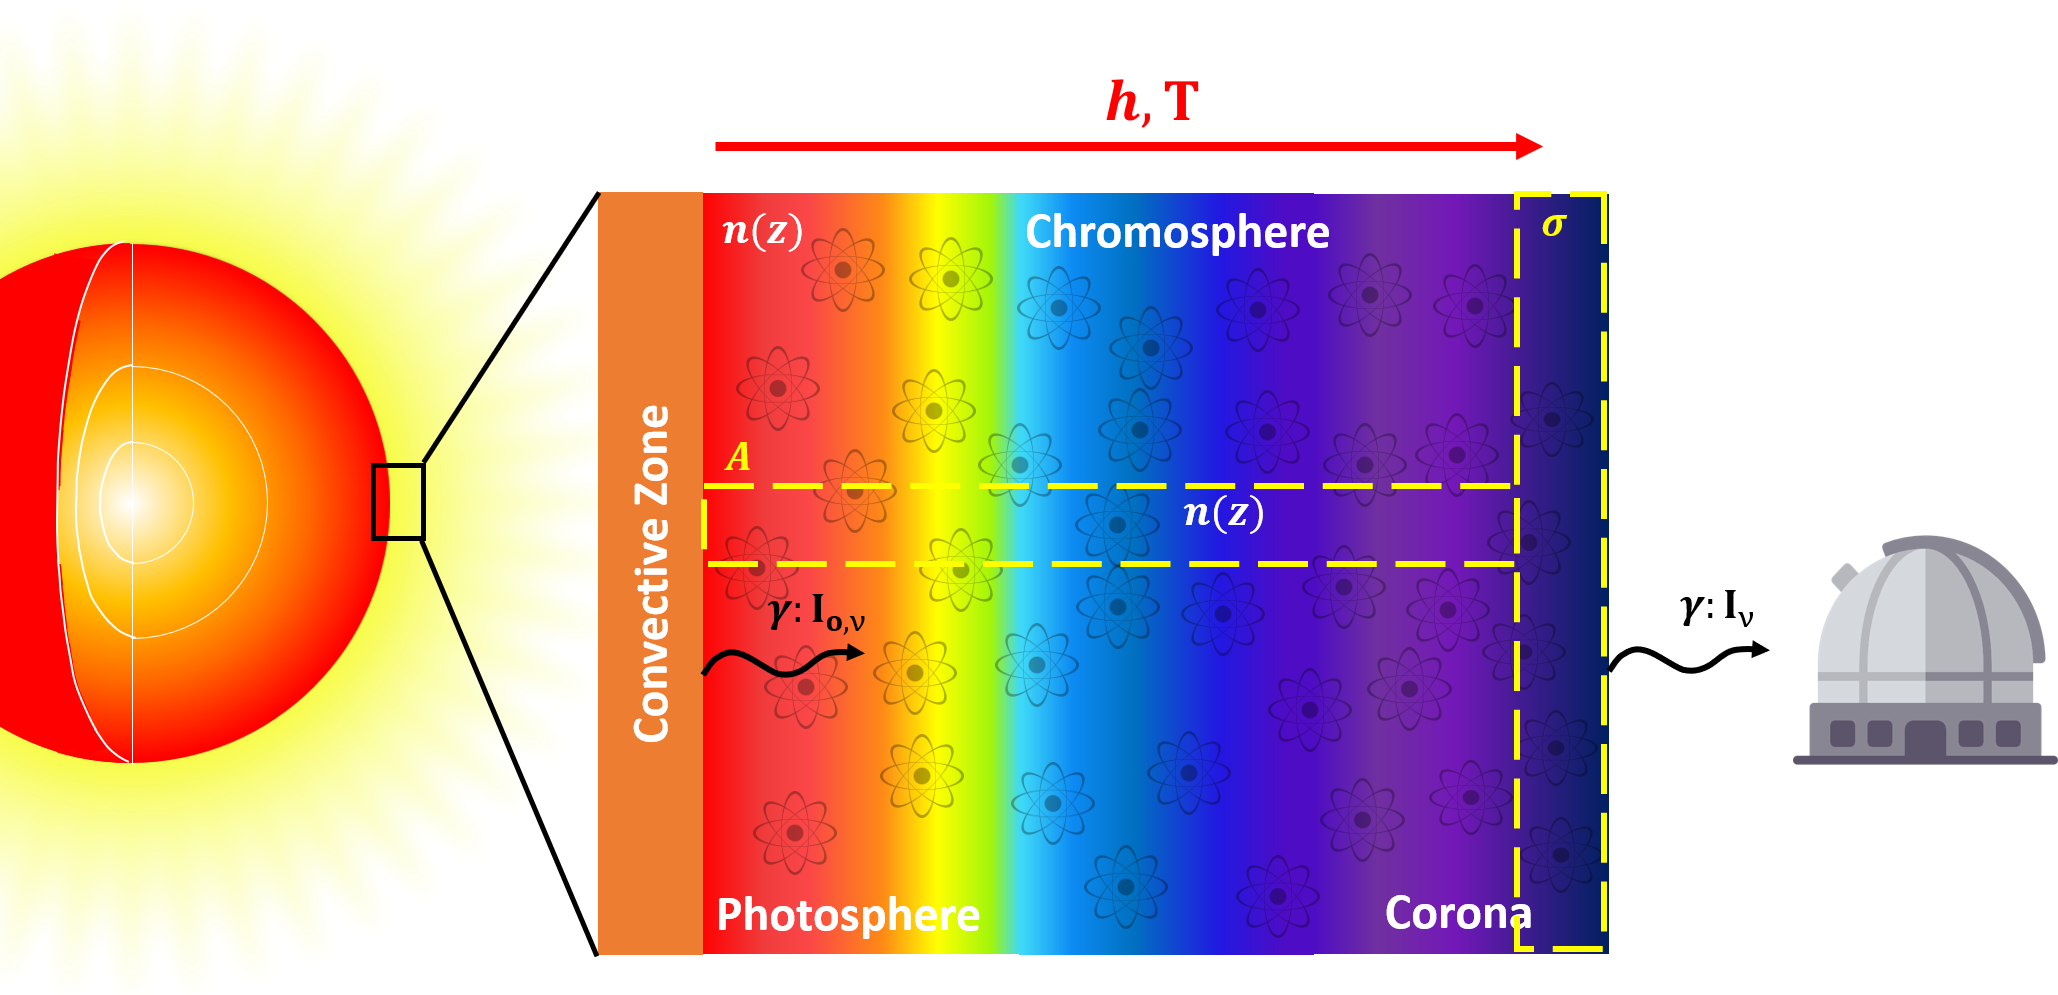
\includegraphics[width=1\linewidth]{Images/densidad_masa (2).png}
    \caption{Representación de la densidad de masa columnar en la atmósfera estelar.}
    \label{fig:rep_dens_masa}
\end{figure}

Si se aplica la ley de absorción pura simple, guiándonos con la figura \ref{fig:rep_dens_masa}, un fotón que viene de la fotosfera con intensidad $I_{o, \nu}$, que es absorbido en su paso por la atmósfera saldrá con una intensidad específica, según la ecuación \ref{ec:ley_abs}. Donde $\tau_{\nu}$ representa la profundidad óptica, que nos da una idea de la opacidad en cierta región específica de la atmósfera \citep{carroll2017introduction}

\begin{equation}
    I_{\nu} = I_{o,\nu} e^{- \tau_{\nu}}.
    \label{ec:ley_abs}
\end{equation}

La profundidad óptica se puede reescribir en términos de las características espectroscópicas que conocemos de las líneas como $\tau_{\nu} = \phi_{\nu} \tau_{o, \nu}$. Donde $\phi_{\nu}$ se conoce como la función del perfil de la línea que se relaciona con la forma de esta y además nos da información sobre las condiciones ambientales en las que se está formando la línea. Además este nuevo $\tau_{o, \nu}$ se puede expresar en términos de la densidad de masa columnar y la sección de área transversal o las probabilidades de transición entre niveles atómicos que absorbieron el fotón (\textit{fg}), como se expresa en la ecuación \ref{ec:prof_opt}.

\begin{equation}
    \begin{array}{cc}
        \tau_{o, \nu} =& N \sigma \\
        \tau_{o, \nu} \propto& N fg \propto A_i
    \end{array}
    \label{ec:prof_opt}
\end{equation}

%%%%%%%%%%%%%%%%%%%%%%%%%%%%%%%
%%%%%%%%%   Section   %%%%%%%%%
%%%%%%%%%%%%%%%%%%%%%%%%%%%%%%%
\section{Curva de crecimiento}\label{CoG}

Los términos mencionados anteriormente, como la densidad de masa columnar y datos atómicos relacionados con las transiciones de niveles energéticos son de gran relevancia para conocer las abundancias químicas y así analizar las atmósferas estelares. Para esto, se puede usar el método de síntesis o \textbf{anchos equivalentes ($W_{\lambda}$)} \citep{jofre2019accuracy}. En este caso, nos enfocaremos en el segundo, que es una medida de la \textit{fuerza} de las líneas espectrales, donde se tiene en cuenta la profundidad y el ancho de la línea respecto al continuo local, como se observa en la figura \ref{fig:ancho_eq}. 

\begin{figure}[h]
    \centering
    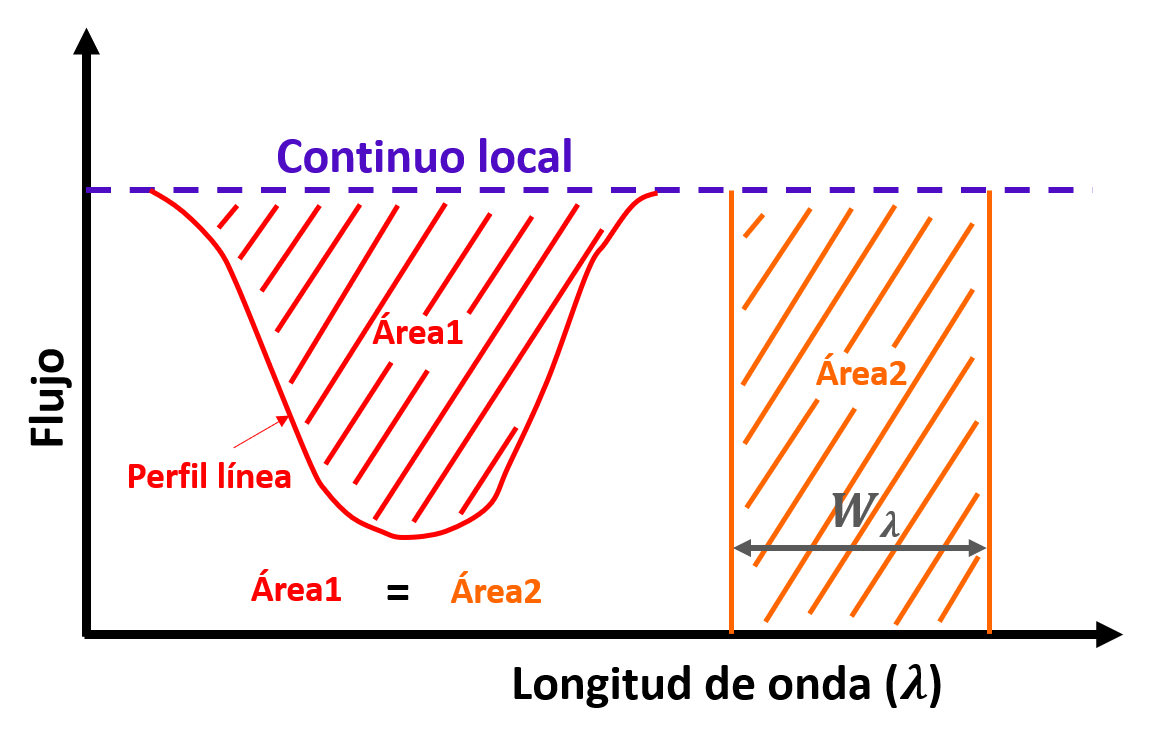
\includegraphics[width=0.6\linewidth]{Images/ew.png}
    \caption[Representación del ancho equivalente de una línea de absorción.]{El ancho equivalente es el ancho de un rectángulo que tiene el mismo área que se encuentra dentro de una línea de absorción teniendo como referencia el continuo local.}
    \label{fig:ancho_eq}
\end{figure}

\noindent Para obtener información de la atmósfera estelar, se pueden crear curvas de crecimiento (CoG). Con estas curvas se quiere conocer cómo cambia el perfil de las líneas de un mismo elemento, es decir, que tan pronunciadas son, lo cual se relaciona directamente con la profundidad óptica, la densidad de masa columnar y el ancho equivalente. Para esto, se gráfica $log(W_{\lambda}/\lambda)$, en el eje \textit{y} y $log(gf)$ en el eje \textit{x}. Donde $f$ es la fuerza del oscilador y $g$ es el peso estadístico del nivel de energía bajo, es decir, son los datos atómicos que dan información sobre la probabilidad que tiene un electrón de hacer una transición de un elemento específico de un orbital atómico a otro según la excitación y condiciones como la temperatura, entre otros. Cabe resaltar, que actualmente estos valores, para la astronomía se pueden extraer de repositorios de datos como ``Vienna Atomic Line Data Base'' (VALD) \citep{piskunov1995vald}, los cuales han sido obtenidos a partir de cálculos semi-empíricos, combinados con datos de laboratorio de alta precisión. Esta base de datos tuvo su última actualización en el año 2019.

En la figura \ref{fig:lines_cog} se observa una representación gráfica de algunos tipos de línea que se pueden encontrar dentro de un espectro estelar. Según \cite{carroll2017introduction}, se pueden tener líneas débiles, fuertes, saturadas y con \textit{damping wings} o gran amortiguamiento en los extremos de la línea. Cada una de estos tipos tiene una relación diferente entre el ancho equivalente (porque tienen perfiles diferentes) y la densidad de masa columnar o las probabilidades de transición, esto se observa en la ecuación \ref{ec:relation_W_fg} para cada una de estas líneas respectivamente.

\begin{figure}[h]
    \centering
    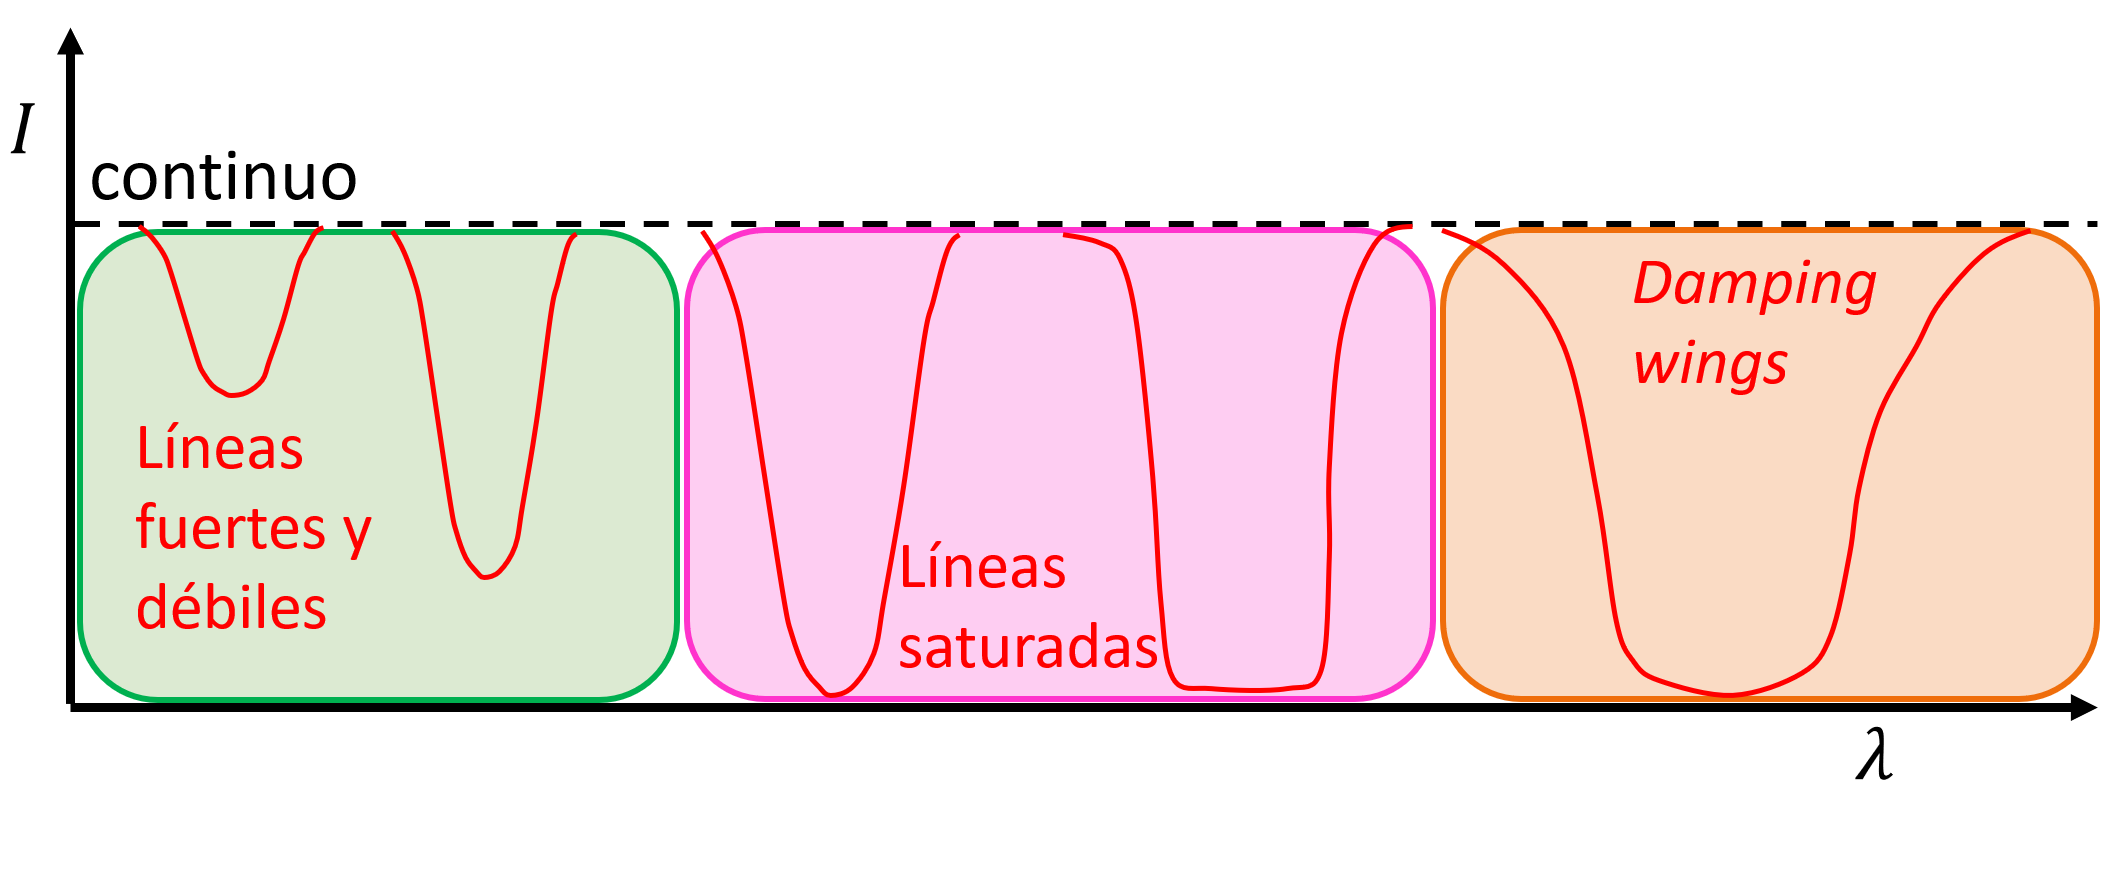
\includegraphics[width=0.9\linewidth]{Images/lineas_goc.png}
    \caption{Representación del tipo de líneas que se pueden encontrar en un espectro.}
    \label{fig:lines_cog}
\end{figure}


\begin{equation}
        \frac{W_{\lambda}}{\lambda} \propto\left\{\begin{array}{l}
        Nfg\lambda \\
        log(Nfg\lambda) \\
        \sqrt{Nfg\lambda}
        \end{array}\right..
        \label{ec:relation_W_fg}
        \end{equation}


\begin{figure}[h]
    \centering
    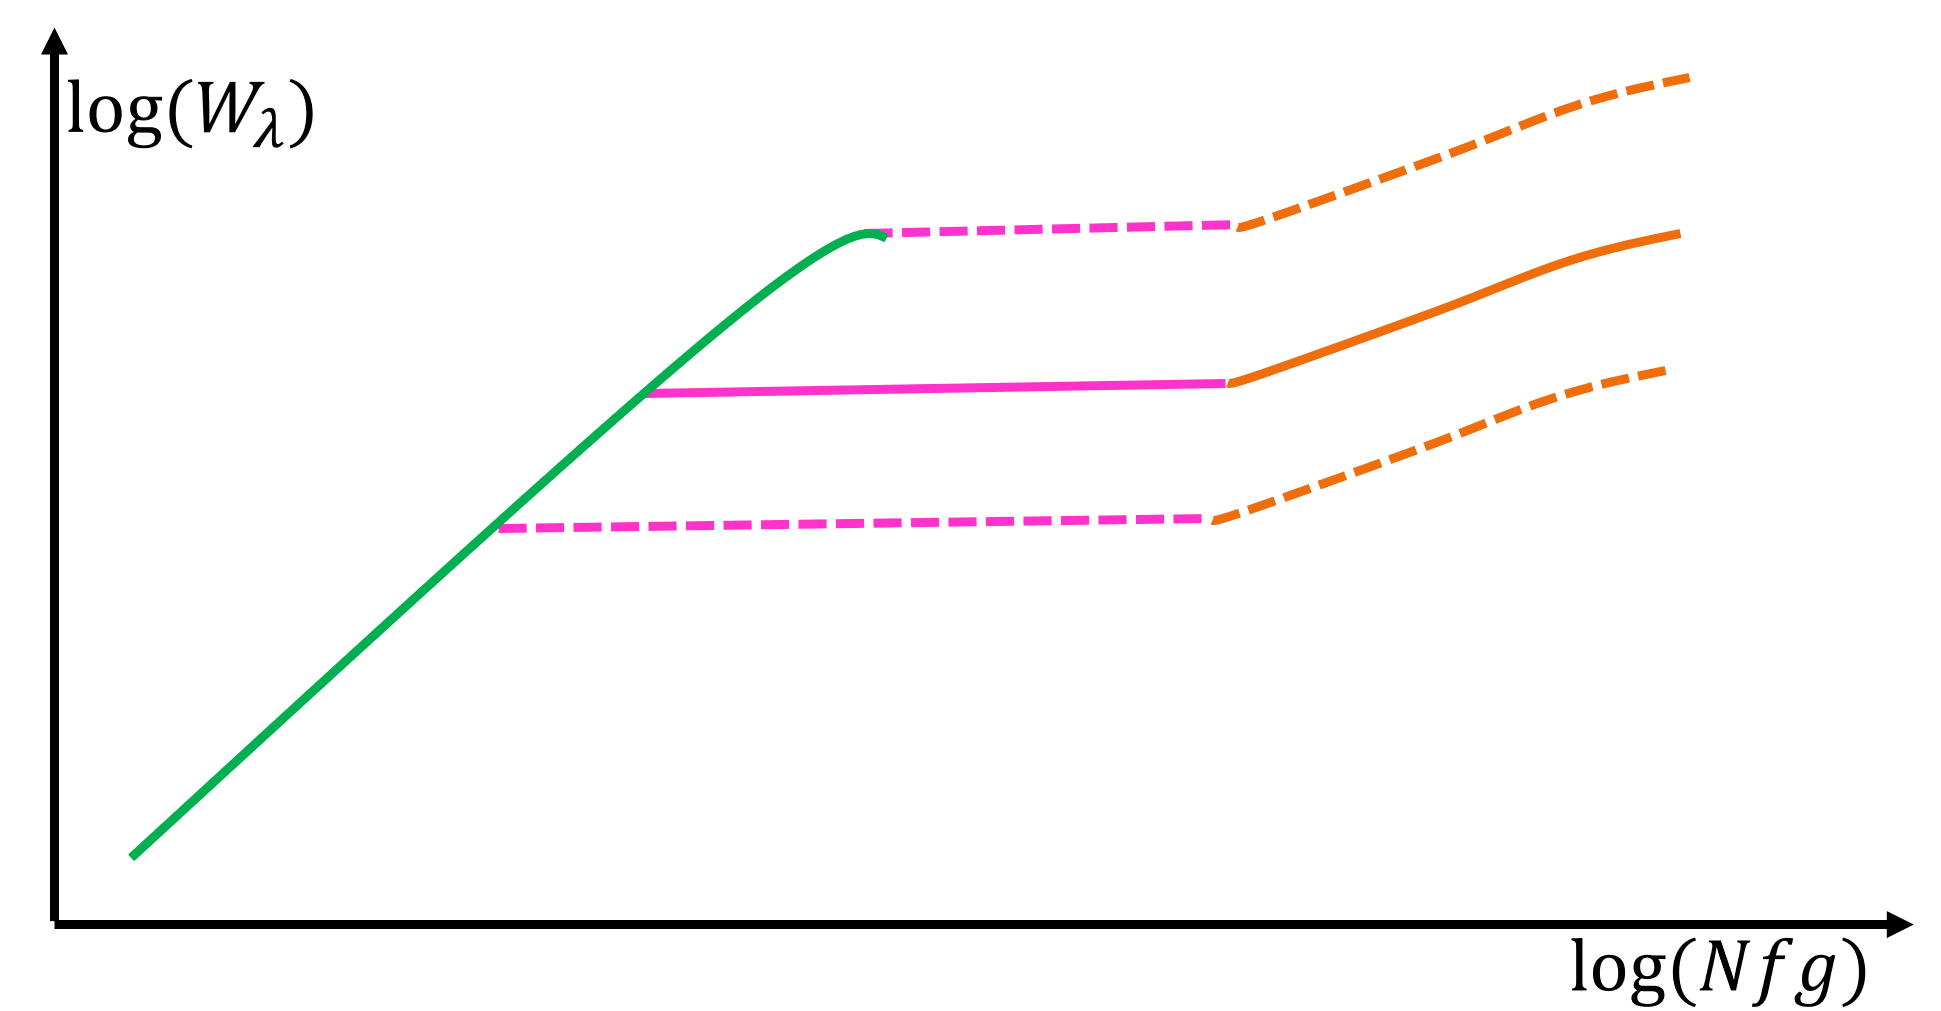
\includegraphics[width=0.75\linewidth]{Images/goc.png}
    \caption{Representación de Curva de crecimiento para un espectro con líneas fuertes, saturadas y con amortiguamiento en sus 'alas'.}
    \label{fig:GoC}
\end{figure}

Estas relaciones, evidencian que según los diferentes perfiles de las líneas, como las de la figura \ref{fig:lines_cog} se tienen diferentes relaciones con la probabilidad de transición y el comportamiento de la densidad de masa columnar. Estas relaciones se pueden apreciar mejor en las curvas de crecimiento. En la figura \ref{fig:GoC} se representa GoC donde se tienen en cuenta los tres tipos de líneas en un mismo espectro. Se observa que para las líneas de absorción fuertes y débiles les corresponde una forma lineal, con pendiente 1:1, esto es debido a debido a la delgadez en la atmósfera. En el caso de líneas saturadas, varían los valores del eje x, manteniendo casi contante los valores de ancho equivalente, debido a la misma saturación. El hecho de observar mayor o menor saturación se relaciona directamente con la velocidad de turbulencia de la estrella. Para líneas fuertes o saturadas con presencia de 'alas' esta cuerva permite medir el amortiguamiento de la atmósfera, donde se observa que esta tiene una pendiente 2:1 y se le conoce como la parte del \textit{damping}.

\begin{comment}

\noindent Esta gráfica de \textit{CoG} experimental u observacional, también puede tener otros valores en el eje \textit{x}, como de densidad de masa columnar, ya que según lo vimos en la ecuación de Saha (\ref{saha}) estos valores son proporcionales.

Pero, esta curva, también se puede hacer teóricamente, ya que de acuerdo a perfiles de líneas gaussiano, lorentziano o deltas invertidos y según esto cada línea tendrá una intensidad que está dado por la ecuación (\ref{ec:intensidad_linea}) donde evidentemente depende de la longitud de onda $\lambda$, la longitud doppler $\Delta \lambda_D$ y la ecuación de Saha $A_i$, como se escribe en la ecuación (\ref{saha}) y se resuelve mediante integración numérica.

\begin{equation}
    I_i = I_0 exp\{-A_i e^{(\frac{\Delta \lambda}{\Delta \lambda_D})^2}\}
    \label{ec:intensidad_linea}
\end{equation}
\end{comment}


Este método de las curvas de crecimiento ha sido empleado en trabajos como \citep{kps1O} y \citep{wilson1954chromospheric} para hacer análisis de densidad de masa columnar en fechas de eclipses anteriores al del 2019. Por lo que se tienen como referente para el análisis que se realiza en esta tesis.




%%%%%%%%%%%%%%%%%%%%%%%%%%%%%%%%%%%
%%%%%%%%%%%%%% CHAPTER %%%%%%%%%%%%
%%%%%%%%%%%%%%%%%%%%%%%%%%%%%%%%%%%

\chapter{Datos Observacionales}  \label{cap:datos_obs}

En este proyecto se hace un análisis tanto teórico como observacional, por lo tanto, se requiere del manejo de conjunto de datos, programas y \textit{scripts} para la manipulación de los mismos. Por lo que es relevante conocer cómo han sido recolectados los datos que se usan, qué repositorios de datos adicionales han sido requeridos y cómo estos se manipularon para hacer los respectivos análisis.

\noindent Principalmente se usan datos de fotometría para definir con precisión las fechas exactas de ingreso y egreso del eclipse. Y datos de espectroscopía tomados por el telescopio TIGRE-HEROS para hacer el análisis de densidad. Además, también se usan datos de repositorios como del \textit{American Association of Variable Star Observers} (AAVSO)\footnote{\url{https://www.aavso.org/data-download}}, de la base de datos astronómica SIMBAD que proporciona datos básicos, identificaciones cruzadas, bibliografía y mediciones para objetos astronómicos fuera del sistema solar y datos atómicos de espectroscopía estelar de \textit{Vienna Atomic Line Database} (VALD) \citep{piskunov1995vald}.

%%%%%%%%%%%%%%%%%%%%%%%%%%%%%%%
%%%%%%%%%   Section   %%%%%%%%%
%%%%%%%%%%%%%%%%%%%%%%%%%%%%%%%

\section{Fotometría}\label{sec:fotometria}
Esta herramienta nos permite conocer el brillo de los objetos astronómicos y para sistemas binarios o planetarios es una herramienta fundamental, ya que observamos cambios en el brillo durante el transito del eclipse. Con estas variaciones, podemos construir la gráfica conocida como \textit{curva de luz}, la cual muestra la intensidad de luz del sistema en función del tiempo; ésto resulta útil para conocer las fechas exactas de cada una de las fases del eclipse.
\vspace{2mm}

\noindent Para la gráfica de la figura \ref{fig:curvaluz}, se usaron datos del repositorio AAVSO, específicamente se tomaron los datos de la banda azul, donde se usó el filtro B Johnson. En esta gráfica se puede observar como varía la magnitud aparente del sistema $\zeta$ Aur durante las fases del eclipse.


\begin{figure}[h]
    \centering
    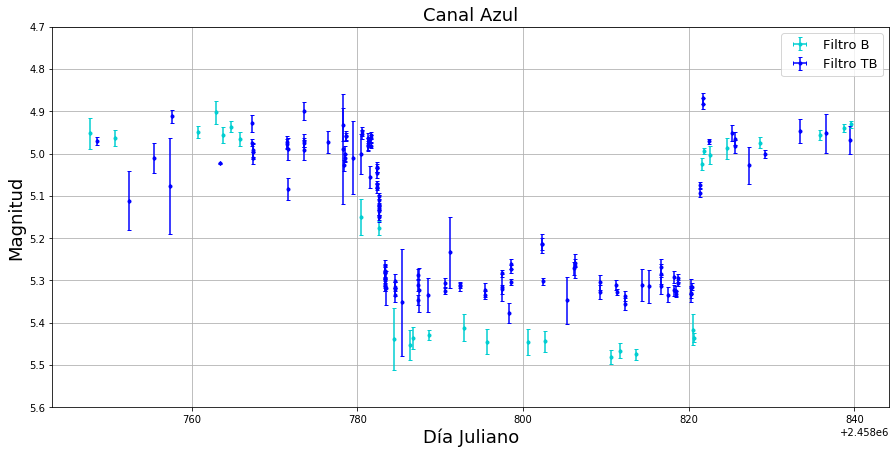
\includegraphics[width=1\linewidth]{Gaficas/curva luz.png}
    \caption[Curva de luz del eclipse del sistema $\zeta$ Aurigae del 2019.]{Curva de luz del eclipse del sistema $\zeta$ Aurigae del 2019, a partir de los datos del repositorio AAVSO: Magnitud aparente vs días julianos. En esta gráfica se tienen fechas desde 21 Septiembre hasta el 22 Diciembre del 2019.}
    \label{fig:curvaluz}
\end{figure}

\noindent Según esta figura \ref{fig:curvaluz}, conocemos las fechas en las que ocurre cada uno de los contactos, esta información está registrada en la tabla \ref{tabla:fechas}. Durante el eclipse total es en el único momento en que se puede observar la estrella gigante de manera individual, ya que la estrella $\zeta$ Aur B se encuentra por detrás según nuestra línea de visión. Además podemos observar que la entrada y la salida no duran lo mismo, porque la gráfica no es simétrica, por lo tanto nos muestra indicios de la excentricidad de la orbita.

\begin{table}[h]
\centering
\begin{tabular}{|c|c|}
\hline
\textbf{Fecha (2019)}    & \textbf{Fase}                                                                   \\ \hline
Antes de 23 octubre      & No hay contacto                                                                     \\ \hline
24 - 26 octubre          & \begin{tabular}[c]{@{}c@{}}Primer contacto y eclipse parcial\\ Ingreso\end{tabular} \\ \hline
27 octubre - 2 diciembre & Eclipse total                                                                       \\ \hline
3 - 4 diciembre          & \begin{tabular}[c]{@{}c@{}}Tercer contacto y eclipse parcial\\ Egreso\end{tabular}  \\ \hline
Después 5 diciembre      & No hay contacto                                                                     \\ \hline
\end{tabular}
\caption{Fechas de cada uno de los contactos del eclipse 2019 de $\zeta$ Aurigae.}
\label{tabla:fechas}
\end{table}

Por otro lado, desde Vienna (Austria), el astrónomo amateur Wolfgang Vollmann, pudo tomar datos de fotometría del ingreso del eclipse de este sistema como se observa en la figura \ref{fig:curva_luz_vienna}. En esta figura se observa que la escala de magnitud es un poco mas alta, debido a que no usó filtros Johnson, sino que se implementó una cámara canon. Con estos datos se pueden terminar de corroborar las fechas del ingreso descritas anteriormente en la tabla \ref{tabla:fechas}.

\begin{figure}
    \centering
    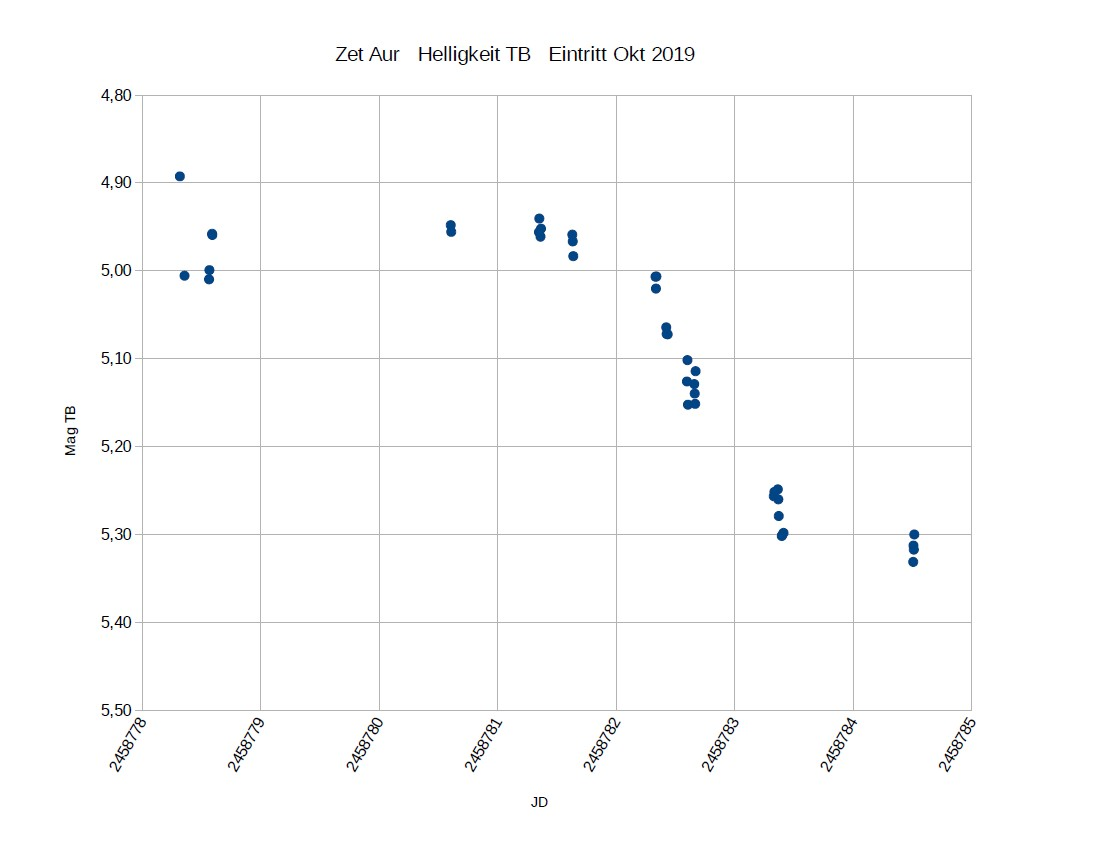
\includegraphics[width=0.7\linewidth]{Gaficas/Zet_Aur_2019_TB_Eintritt_20191028.jpg}
    \caption[Curva de luz del ingreso del eclipse del sistema $\zeta$ Aurigae del 2019]{Curva de luz del ingreso del eclipse del sistema $\zeta$ Aurigae del 2019, con datos de un astrónomo amateur en Vienna.}
    \label{fig:curva_luz_vienna}
\end{figure}



\subsection*{Altitud y proyección geométrica}

Con los datos de las curvas de luz es posible obtener la altitud proyectada del centro de la estrella $\zeta$ Aur B sobre la estrella $\zeta$ Aur A. Esto nos muestra que para el JD 2458782.6 $\pm$ 0.1d, Octubre 26 de 2019, a las 2:20h UTC tenemos la altura $h=0$ del ingreso. Lo cual representa que la estrella en secuencia principal está oculta a la mitad (50\%), como se observa en la figura \ref{fig:altura_proyec}.

Para la fecha del egreso se tiene que esta altura $h=0$ es el JD 2458821.0 $\pm$ 0.2d, es decir, Diciembre 03 de 2019, 12h UTC. Con esta información conocemos las fechas en que tenemos espectros combinados con líneas cromosféricas y las fechas de solo espectros puros de la estrella gigante. Además es posible conocer las alturas proyectadas de los espectros combinados del eclipse de 2019 y es posible hacer análisis y comparaciones con las alturas proyectadas del eclipse de 1987.

Para poder conocer las fechas más exactas del ingreso, la altitud y las alturas proyectadas de cada una de las fechas, es necesario recordar que con la velocidad transversal relativa de las dos estrellas y la duración del eclipse se obtiene la longitud de arco que atraviesa la estrella $\zeta$ Aur B por detrás de la estrella $\zeta$ Aur A. Una representación gráfica de los conceptos más relevantes que implementamos para el cálculo de las alturas se observa en la figura \ref{fig:altura_proyec}. Conociendo que la velocidad tangencial relativa está dada por la ecuación \ref{ec:vel_Tan}

\begin{equation}
    V_{tan-rel} = (1 + q)V_{tan-\zeta A}.
    \label{ec:vel_Tan}
\end{equation}

\begin{figure}[h]
    \centering
    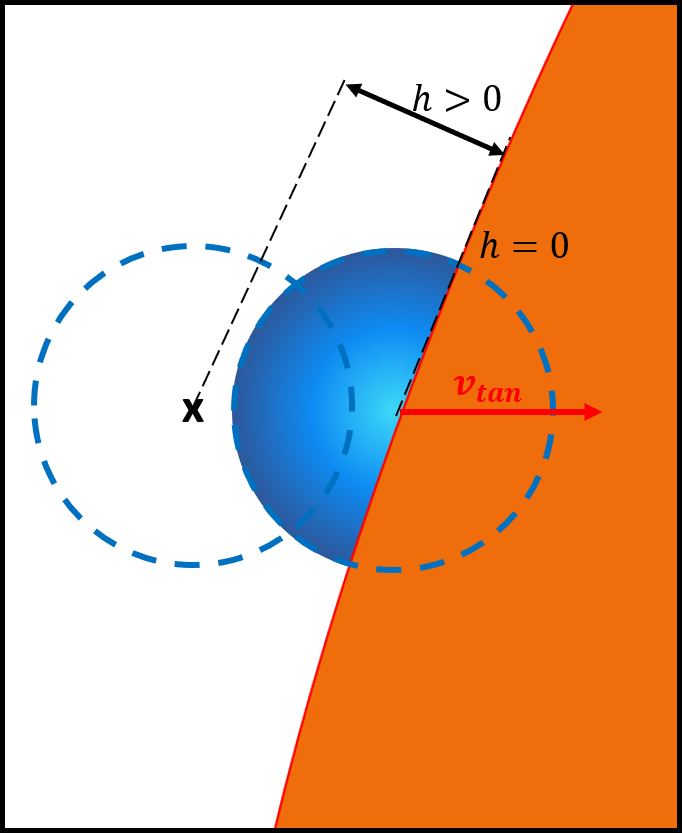
\includegraphics[width=0.5\linewidth]{Images/altura_proyec.png}
    \caption{Representación de la altura proyectada en las fases de eclipse parcial.}
    \label{fig:altura_proyec}
\end{figure}

Teniendo en cuenta la bibliografía consignada en en la tabla \ref{tabla:parametroz_a} del capítulo \ref{cap:zetaaur}, es posible deducir $V_{tan-rel} = 65.5 km/s$. Pero es necesario tener en cuenta que la velocidad tangencial disminuye hasta 1.5 km/s en la mitad del eclipse, entonces se asume $V_{tan-rel} = 65 km/s$, al igual que en \citet{kps9}.

Con esto, tenemos que la longitud de arco a mitad es de 155.0097$ R_{\odot}$ y la latitud ($\phi$), está dada por

\begin{equation*}
    \phi = cos^{-1}\left(\frac{\Delta S}{R_{\zeta A} - R_{\zeta B}}\right).
\end{equation*}

Donde $\Delta S$ es la mitad de la longitud de arco que recorre la estrella $\zeta$ Aur B durante el eclipse total. Con esto obtenemos $\phi =$ 15.55° y por último, obtenemos cuánto dura el ingreso de acuerdo a $2R_{\zeta B} sec (\phi)$ lo que da 1.31 días.

\noindent Por último, teniendo en cuentas estas fechas, es posible saber cuáles son los espectros que se implementarán para hacer un análisis de densidad de masa columnar y cuál es la altura proyectada de cada una de estas fechas. Para esto entonces, nos regimos por:

\begin{equation*}
    h = \Delta t \cdot V_{tan-rel}.
\end{equation*}

Donde esta diferencia de tiempo es respecto a la altura $h = 0$, por lo que teniendo en cuenta dos espectros del ingreso, sus respectivas alturas proyectadas son de $\num{1.02e7}$ km el 24 de Octubre y $\num{4.39e6}$ km el 25 de Octubre.





%%%%%%%%%%%%%%%%%%%%%%%%%%%%%%%
%%%%%%%%% Section  %%%%%%%%%
%%%%%%%%%%%%%%%%%%%%%%%%%%%%%%%
\section{Espectroscopía} 
La herramienta fundamental en este proyecto es la espectroscopía, por lo que dentro de la metodología resulta necesario explicar cómo se tomaron las datos, que incluye la instrumentación y cómo se van a manejar estos datos para obtener resultados favorables y cumplir los objetivos propuestos.

\subsection*{Telescopio TIGRE - HEROS}

Este proyecto está en convenio con la Universidad de Guanajuato en México y esta universidad cuenta con el telescopio TIGRE, por sus siglas Telescopio Internacional de Guanajuato Robótico Espectroscópico, el cual tiene un convenio bilateral con la Universidad de Hamburgo - Alemania y la Universidad de Liège - Bélgica. Este telescopio fue originalmente denominado ``Hamburgo Robotic Telescope  (HRT)'' en 2005, cuando fue entregado a la Universidad de Hamburgo para hacer pruebas. Pero debido a limitaciones climáticas en el cielo alemán, el telescopio fue reinstalado en su sitio final, el Observatorio La Luz en septiembre de 2012, a una altitud de 2400 m sobre el nivel del mar en una meseta alta al norte de la ciudad de Guanajuato \citep{schmitt2014tigre}. En la figura \ref{fig:tigre-heros} se observa los componentes de este observatorio.

\noindent Este telescopio se concentra principalmente en física estelar. Tiene óptica Cassegrain-Nasmyth, el espejo primario tiene una apertura de 1.20 m, con distancia focal de 3.6 m, y el secundario alarga el foco a 9.6 m, por lo que es un sistema f/8, todos los dispositivos y software están diseñados para uso robótico remoto.

\begin{comment}
\noindent El observatorio La Luz, también está conformado por un espectrógrafo, el cual para la calibración al telescopio se necesita un adaptador que alimente la luz de una estrella o de las lámparas de calibración. El telescopio se conecta con una fibra multimodo de sílice fundida con un diámetro de núcleo de 50 $\mu $ directamente al espectroscopio Echelle, con relación focal de f / 4.5 del colimador del espectrógrafo en su salida; como esta fibra tiene un largo de 15 m, ya que está ubicado en una habitación separada con clima controlado;  en su interior tiene microlentes integrales, basados en láser para minimizar las pérdidas de luz.
\end{comment}


\noindent El espectrógrafo fue construido mediante la restauración del espectrógrafo HEROS, por sus siglas en inglés Heidelberg Extended Range Optical Spectrograph. Se tiene dos cámaras, una para el canal rojo y una para el azul, las cuales tienen un píxel de tamaño de 13.5 $\mu m$ por lo que precisión instrumental está únicamente por el ruido de lectura. Dentro del espectrógrafo, la luz primero pasa el colimador, luego por la rejilla echelle. Detrás de este último, se divide en dos haces de luz (luz azul y roja) a través de un divisor de haz dicroico.  El haz de luz azul cubre un rango de longitud de onda de $\approx$ 3750–5700 \r{A} y el haz rojo un rango de longitud de onda de $\approx$ 5830–8800 \r{A}.

\noindent El poder de \textit{resolución espectral} $\lambda / \Delta \lambda$ es aproximadamente de 20000 y fue calculado mediante calibraciones con una lámpara de ThAr. Además, aunque la \textit{relación señal a ruido} (SNR) depende de las condiciones climáticas y de la distribución de energía espectral de la fuente, según pruebas con estrellas estándar este valor se mantiene superior a 100 en la mayoría de los espectros recolectados. 

\begin{figure}
    \centering
    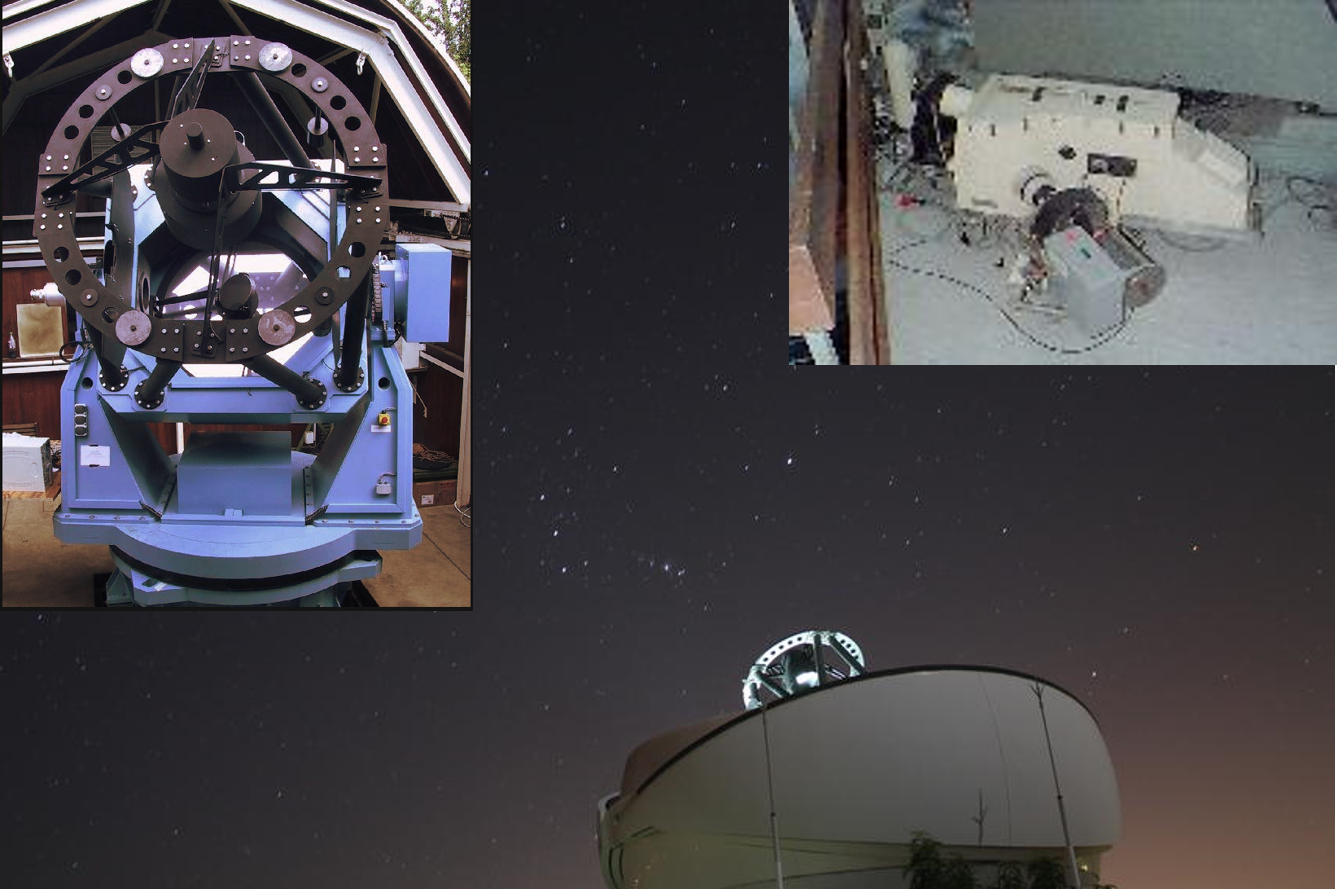
\includegraphics[width=1\linewidth]{Images/TIGRE-HEROS.png}
    \caption[Instrumentación implementada para los obtener los datos de espectroscopía usados en este proyecto]{Instrumentación implementada para los obtener los datos de espectroscopía usados en este proyecto. Observatorio La Luz, el telescopio TIGRE al costado superior izquierdo y el espectrógrafo HEROS en el costado superior derecho.}
    \label{fig:tigre-heros}
\end{figure}


\noindent Todos los datos espectroscópicos fueron tomados por el TIGRE-HEROS en las fechas comprendidas entre el septiembre y diciembre del año 2019 mientras ocurría el eclipse del sistema $\zeta$ Aur. Además estos datos fueron reducidos y están en formato \texttt{FITS}, que según sus siglas en inglés significa, Flexible \textit{Image Transport System}, que en Astronomía es el formato estándar \citep{hanisch2001definition} de intercambio y archivo de datos. El nombre de cada archivo especifica la fecha en que fueron tomados los datos y el canal al que perteneces, azul o rojo. Por cada fecha y canal hay un archivo $\_ main\_$ que contiene los datos, y un archivo $\_ small\_$ que contiene información relevante como las condiciones ambientales entre otros. Estos paquetes de datos son descargados directamente de la página de la Universidad de Hamburgo.

\section{Reducción de datos}

Para hacer manipulación de los datos en el programa iSpec y algunos códigos de Python, es necesario y facilita el trabajo usar archivos \texttt{.dat}. Por lo que es necesario hacer una conversión de los archivos \texttt{.fit}. Para esto se empleó un código llamado \texttt{DataRedu}, el cual emplea los archivos de conversión original creados en Hamburgo\footnote{Ver el manual de usuario del Telescopio TIGRE-HEROS en la sección Software: \url{https://hsweb.hs.uni-hamburg.de/projects/TIGRE/EN/hrt_user/python_soft.html}} de forma recursiva sobre todo el conjunto de archivos. Esta modificación y creación del código texttt{DataRedu}, se encuentra en los anexos de la tesis de maestría \citep{Faiber2019master}.


\noindent El código es muy eficiente ya que no es necesario pasar por cada uno de los paquetes de datos sino que está optimizado para hacer la conversión de carpetas de datos completas, bajo algunas especificaciones. Además, genera un archivo que contiene el contenido de la tabla \ref{Tabla:DataRedu}, el cual es muy útil para el uso de algunos códigos, ya que me muestra explícitamente cual es la resolución de cada uno de los sets de datos. Una explicación más detallada del funcionamiento y modificaciones están en el repositorio Github de este proyecto\footnote{ Link de repositorio en Github: \url{https://github.com/ntlucia/Tesis_Estrellas_binarias/tree/master/Scripts/DataRedu}}.

\begin{table}[h]
\centering
\resizebox{15cm}{!} {
\begin{tabular}{|c|c|c|c|c|}
\hline
\textbf{SPECTRUM}                                     & \textbf{CHANNEL}                                                     & \textbf{RESOLUTION}                                                                               & \textbf{SNR}                                                               & \textbf{IRF}                                                                             \\ \hline
Nombre del archivo                           & \begin{tabular}[c]{@{}c@{}}Canal\\ rojo - azul\end{tabular} & \begin{tabular}[c]{@{}c@{}}Resolución del \\ telescopio y \\ espectroscopio\end{tabular} & \begin{tabular}[c]{@{}c@{}}Relación \\ señal a ruido\end{tabular} & \begin{tabular}[c]{@{}c@{}}Función de \\ respuesta \\ instrumental\end{tabular} \\ \hline
zetaAur-eclipse\_R\_2019\_11\_19\_02\_52\_08 & R                                                           & 20538                                                                                    & 496.82                                                            & 21.08                                                                           \\ \hline
zetaAur-eclipse\_B\_2019\_11\_19\_02\_52\_08 & B                                                           & 20652                                                                                    & 109.66                                                            & \textbf{}                                                                       \\ \hline
\end{tabular}}
\caption{Información de los espectros obtenida con el código DataRedu.}
\label{Tabla:DataRedu}
\end{table}

\noindent Algo muy relevante de estos datos y el \textit{script} de reducción, es que se tiene la opción de hacer una corrección en flujo, para eliminar el continuo instrumental que no tiene relevancia física. En esta corrección se aplica la técnica denominada “rectificación del continuo” la cual es necesaria para poder hacer comparaciones y operaciones entre espectros. Pero como se observa en la figura \ref{fig:espectro_puro}, esta normalización no es muy confiable. En la región de 425 - 450 [nm] se observa un pico  “artificial'' que no corresponde con lo que se debería esperar en el espectro puro de la estrella gigante (al compararlo con un espectro sintético de una estrella con los mismos parámetros estelares). En 1987 se tuvieron problemas de normalización debido a este pico que no se explicaba físicamente, por lo que se usaban líneas de absorción inferiores a ese valor, para no introducir errores significativos.

Además se observa otro pico entre 480-520 [nm] del espectro combinado. Por lo que es necesario revisar con más detalle esta normalización, lo cual es mencionado en la sección \ref{sec:normalizacion} . Ya que al parecer las normalizaciones hechas por este código funcionan mejor para estrellas en secuencia principal, ya que emplea el código de modelado de atmósferas PHOENIX \citep{husser2013new}, que no tiene en cuenta efectos como el \textit{line blacketing} que afecta de manera significativa estrellas gigantes. Además también se ajusta mejor al canal rojo, ya que en este las estrellas gigantes no tienen tantas líneas fuertes y el SNR es mayor.

\begin{figure}[h]
    \centering
    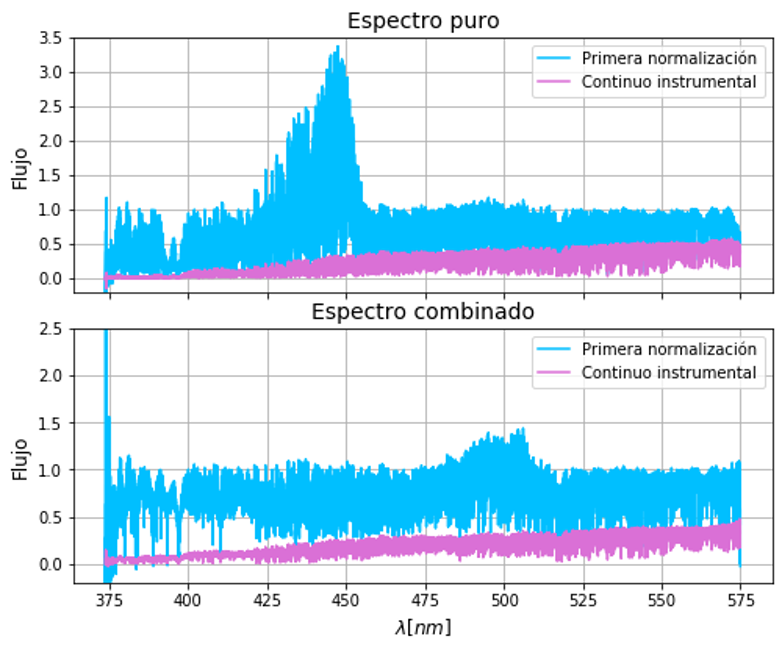
\includegraphics[width=0.9\linewidth]{Gaficas/primer_normal.png}
    \caption{Espectro puro de la estrella gigante roja del sistema binario Zeta Aurigae, el 19 de Noviembre del 2019 y espectro combinado durante el ingreso del eclipse, el 24 Octubre del 2019.}
    \label{fig:espectro_puro}
\end{figure}

\section{Normalización de espectros}\label{sec:normalizacion}

\noindent La manipulación de datos espectrales inicialmente es para tener indicadores de una buena normalización, ya que según \citet{jofre2017gaia}, ésta es una fuente común de incertidumbres. Esta se puede hacer por ajuste de \textit{splines} o polinomios en regiones particulares sin tener en cuenta las líneas de absorción o emisión. Pero como se mencionó en la sección anterior, aún no se logra con los códigos disponibles hasta la actualidad. Por lo tanto, es necesario recurrir a la creación y comparación de espectros sintéticos y a partir del cálculo de parámetros estelares que corroboren el comportamiento de la estrella a analizar. Para esto, usamos recursos y librerías del programa \textit{iSpec}.

\subsection*{iSpec}
\label{sec:para_est}

\noindent El programa iSpec basado en Linux, hecho por \citet{blanco2014determining} tiene la función de hacer análisis espectral y calcular parámetros físicos y estelares, teniendo en cuenta las especificaciones de la sección \ref{sec:para_est}. En el programa se tienen en cuenta códigos de transferencia radiativa, para crear espectros sintéticos o calcular abundancias por anchos equivalentes. Además éste puede interactuar con otras aplicaciones como TOPCAT para graficar y manipular catálogos astronómicos; VOSpec, para análisis espectral y fotométrico; y Splat para mostrar, comparar, modificar y analizar espectros. En general, con iSpec, se puede acceder al Observatorio Virtual, que es un repositorio de datos de proyectos a nivel mundial.
\vspace{2mm}

\noindent El proceso de análisis se podría dividir particularmente en dos partes, para el canal azul y el canal rojo. Sin embargo, en este proyecto se hace un énfasis en el procedimiento del canal azul, ya que es donde se encuentran las líneas de absorción más pronunciadas. A partir de la espectroscopía se pueden obtener abundancias químicas estelares, las cuales permiten conocer características de poblaciones estelares, patrones químicos y evolución química de elementos por canales de nucleosíntesis. Para conocer estas abundancias hay que seguir una serie de pasos los cuales permiten conocer y analizar las atmósferas estelares y los parámetros que influyen en estas.



\noindent Inicialmente lo primero que se debe tener claro es el tipo de estrella que se quiere analizar, en este caso se trata de una estrella gigante y su compañera en secuencia principal. Ahora, también es necesario tener en cuenta las posibles incertidumbres que contienen los datos y el proceso de manipulación de los mismos y de acuerdo a esto, conocer qué tan confiables son los resultados.
\vspace{2mm}

\noindent Dos de las características más relevantes en los instrumentos con que se toman los datos son la \textit{resolución} y la relación señal a ruido (\textit{S/N}). Las cuales se deben buscar de acuerdo a lo que se quiere observar, por ejemplo, si se tiene baja resolución es positivo por el tiempo de observación requerido, pero si se quieren encontrar variaciones mínimas en estrellas u obtener perfiles de líneas de emisión o absorción se requiere de una alta resolución. Por otro lado, la S/N $>$ 200 da mucha confianza, pero comúnmente esta se encuentra entre 60-100 en telescopios terrestres y funciona para el tipo de estrellas FGK, que es con lo que contamos en este proyecto.
\vspace{2mm}


Para la manipulación de datos, lo primero que se debe tener es una calibración en longitud de onda $\lambda$, teniendo en cuenta velocidades radiales. Esto se logra ajustando un modelo de polinomios de segundo orden y ajustes gaussianos junto a una lista de mascaras de líneas llamada \textit{VALD.Sun.300\_1100nm} que se ajusta bien para este tipo de estrellas, como se observa en la figura \ref{fig:vel_radial}. También es necesario eliminar líneas telúricas que pueden afectar el espectro debido a la luz proveniente de la estrella que al atravesar la atmósfera terrestre es absorbida y como esta está compuesta por moléculas, se observan líneas características que son dobles, repetitivas, fuertes. Según \citep{bertaux2014tapas} hay estándares o modelos telúricos con los cuales se pueden eliminar estas líneas que afectan el espectro, para evitar errores en la manipulación. 

\begin{figure}[h]
    \centering
    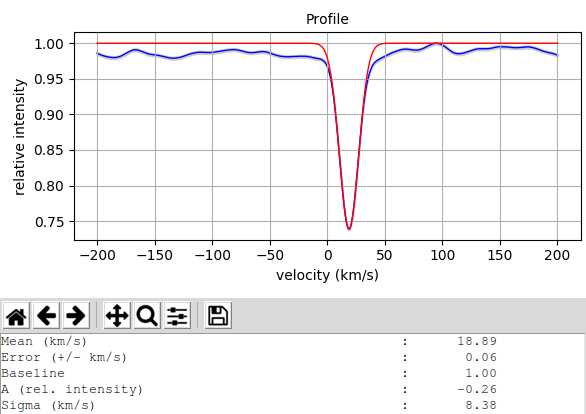
\includegraphics[width=0.8\linewidth]{Images/correct_vel_rad.PNG}
    \caption{Perfil de velocidad radial para hacer correcciones de longitud de onda en los espectros del sistema $\zeta$ Aurigae.}
    \label{fig:vel_radial}
\end{figure}

Para hacer una normalización teniendo en cuenta solo el continuo, es necesario conocer a qué se debe la presencia de las líneas en el espectro. Para conocer esta formación, es necesario tener en cuenta cálculos de transferencia radiativa debido a que las transiciones atómicas son muy complejos debido a la interacción de electrones con los campos de radiación, donde se tienen en cuenta excitación e ionización. Para esto, es necesario crear modelos de atmósfera, según geometrías se pueden emplear principalmente dos: Plana-paralela, para el caso de estrellas enanas; o esférica por capas, para estrellas gigantes, ya que se necesita tener en cuenta la curvatura de atmósferas extendidas. Como nuestro caso es el segundo, se usa el modelo \textit{MARCS.GES}, el cual admite una geometría esférica y el repositorio de abundancias \textit{GREVESS.2007} \citep{grevesse2007solar}.


Además es necesario determinar las líneas espectrales estelares, que \textbf{iSpec} se cuenta con la lista de líneas \textit{VALD.Sun.300\_1100nm}, que es una de las más actualizada y precisa para estrellas gigantes. Estas se pueden analizar por medio de perfiles gaussianos o perfiles de Voigt y con esto resolver ecuaciones de transferencia y hallar flujos continuos y netos. 


\noindent Para análisis de transferencia radiativa y modelos atmosféricos se puede por dos métodos principalmente, uno de ellos el \textit{Equilibrio termodinámico no local} (no-LTE), teniendo en cuenta la geometría y el equilibrio estadístico. Sin embargo, las estrellas no son una ``caja ideal'' por lo que no se obtiene un solo flujo o temperatura, sino un rango de estos, así que hay que tener mucho cuidado con las delimitaciones que se hacen para conservar el equilibrio termodinámico. Otro método es por \textit{tratamiento de opacidades por muestreo}, que es teniendo en cuenta simulaciones hidrodinámicas de la atmósfera, donde se tiene un haz de luz paralelo y cualquier proceso que elimine fotones es absorción colectiva. Donde se tiene en cuenta el scattering, la absorción real de fotones por transiciones de electrones atómicos y en gases frío por transiciones de nivel de energía molecular. Es decir, se tiene en cuenta la \textbf{opacidad}, la cual es función de la composición, la densidad y la temperatura. Según \citep{steffen2013micro} lo ideal es poder hacer análisis en 3D y no-LTE, por lo que en \textbf{iSpec} se usa el código \textit{TURBOESPECTRUM}, que es de síntesis de espectro 1D no-LTE y cubre 600 moléculas, éste es rápido con muchas líneas y utiliza el tratamiento de ampliación de línea descrito por \citep{plez2012turbospectrum}.


\noindent El método de síntesis espectral permite ajustar el espectro observado a uno estándar generado al variar parámetros y disminuyendo el $\chi^2$ entre los dos. Con este nuevo espectros normalizado se calculan los parámetros estelares, partiendo de los registrados en catálogos como PASTEL, \citep{soubiran2016pastel}. Éste es la compilación bibliográfica de parámetros atmosféricos estelares basados en espectroscopia de alta resolución y alta señal a ruido. Estos parámetros son los siguientes:

\begin{itemize}
    \item[1.] \textbf{Temperatura efectiva ($T_{eff}$)}  se obtiene de la ley de Steffan-Boltzmann, con la ecuación (\ref{stefan-boltzman}), la cual se define de manera única para un nivel específico dentro de la estrella y es uno de los descriptores global importante de la estrella. Es muy importante no confundir esta deducción con la \textit{temperatura de excitación} la cual está definida por la ecuación de Boltzmann (\ref{eq:Boltzmann_real}), la \textit{temperatura de ionización} definida por la ecuación de Saha (\ref{saha}), la \textit{temperatura cinética} que se obtiene de la distribución de velocidades de Maxwell-Boltzmann (\ref{eq:boltzmann}) y la \textit{temperatura de color} que se obtiene del ajuste a la forma del espectro continuo de la función de Planck (\ref{ley_planck}). Estas otras temperaturas, diferentes a la efectiva tienen una posición específica en la atmósfera y varían según las condiciones del gas, que en el caso de gas ideal son la misma, debido a que las estrellas se asumen como cuerpo negro y con equilibrio térmico, por lo que una sola temperatura, las describe bien.
    
    \noindent Según las mediciones de este parámetro, la mejor precisión que se tiene de esta medida son 50 [K] y se puede calcular por diversos métodos como balances de excitación o interferometria.
    
    \item[2.] \textbf{Gravedad superficial (log[g])} es la aceleración gravitacional experimentada en la superficie del ecuador, incluidos los efectos de la rotación. Para esta propiedad, no se pueden hacer mejores mediciones que 0.1 dex, y se tiene una una dispersión promedio de 0.25 dex. Esta se puede medir por métodos como paralaje o ionización. 
    
    \item[3.] \textbf{Metalicidad} describe la abundancia relativa de elementos más pesados que el helio en la estrella, esta se puede escribir como [Fe/H] midiendo la abundancia de hierro con respecto a la del hidrógeno, pero no siempre basta con el hierro, sino que en ocasiones también es necesario tener en cuenta los metales en general, entonces es [M/H].

    \item[4.] \textbf{Microturbulencia ($v_{mic}$)} es otro parámetro relevante, la cual representa los movimientos turbulentos a pequeña escala que conducen con el ensanchamiento de las líneas. Se relaciona con densidades ópticas < 1.
    \item[5.] \textbf{Macroturbulencia ($v_{mac}$) y velocidad de rotación proyectada ($v sin[i]$)}, la  primera representa los movimientos turbulentos a gran escala en las atmósferas, como la actividad de la estrella, teniendo en cuenta excitación de átomos, movimientos de convección y divergencia de vientos. La segunda hace referencia a la velocidad de rotación pero teniendo en cuenta la inclinación según el plano de observación. Estos dos parámetros realmente no son fácil separar, ya que sus contribuciones al ensanchamiento de las líneas es similar.
\end{itemize}


\noindent Cabe resaltar que para este proyecto se tienen dos tipos de espectros característicos. Inicialmente, el espectro durante la fase de eclipse total que es el espectro puro de la estrella gigante roja. Y en las fechas de eclipse parcial tenemos el espectro combinado de la estrella gigante y la estrella en secuencia principal. Éste último además de líneas de las dos estrellas, posee líneas producto de la absorción de la luz de la estrella $\zeta$ B en la cromósfera de la estrella $\zeta$ A. Por lo que estos se tienen que normalizar de manera diferente. Es diferente manipular datos de una estrella en específico a la que le conocemos sus parámetros estelares gracias a la bibliografía, que trabajar con un espectro que tiene componentes de dos estrellas.


Para realizar esta normalización, en este proyecto se implementa un \textit{script} en Python llamado \textbf{iSPar}, que emplea funciones del programa iSpec \citep{blanco2019modern}, como se mencionó anteriormente, el cual tiene como fin último el cálculo de parámetros estelares. Por lo que funciona muy bien para el caso del espectro puro de la estrella gigante, comparando con el espectro sintético.

\begin{figure}[h]
    \centering
    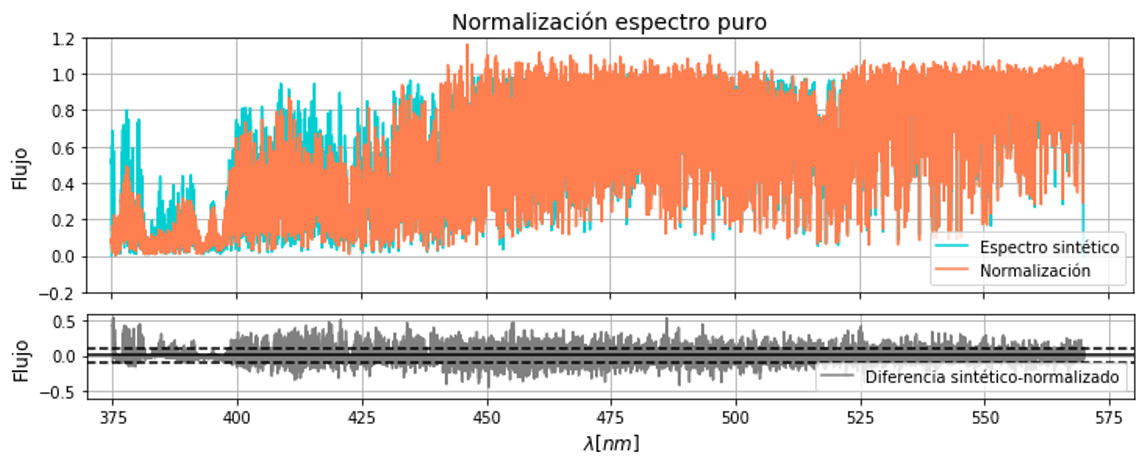
\includegraphics[width=1\linewidth]{Gaficas/comparacion_normalizacion.png}
    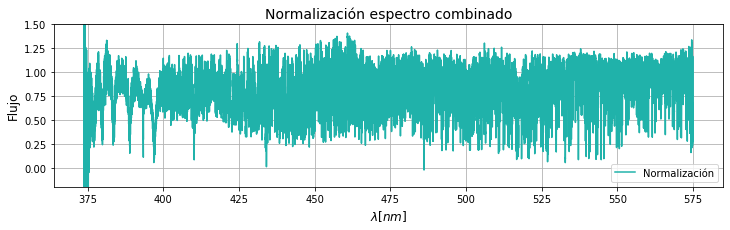
\includegraphics[width=1\linewidth]{Gaficas/normal_comb2.png}
    \caption[Normalizaciones del espectro puro y espectro combinado del eclipse del 2019. ]{Comparación de la normalización del espectro puro respecto al espectro sintético de una estrella gigante tipo K. Normalización del espectro combinado ignorando el \textit{line blanketing} de la estrella gigante.}
    \label{fig:normalizacion}
\end{figure}

Como vemos en la gráfica de la figura \ref{fig:normalizacion} para las regiones inferiores 450 [nm] no se puede tener un valor constante del continuo, sino que esa porción del espectro de la estrella parece reducida en flujo y se debe a que hay la gran cantidad de líneas de absorción por la presencia de metales. Ya que a pesar de que el espectrógrafo tiene una resolución de aproximadamente 20000 no se pueden estudiar todas las líneas individuales, sino que se reduce la intensidad del continuo, debido al efecto de \textit{line blanketing}. Además que al hacer comparaciones con el código \texttt{PHOENIX}, el espectro puro, tiene concordancia con esa caída en 400 nm para las estrellas gigantes como en este caso.

Para el caso del espectro combinado, obtenido durante el eclipse parcial, como no se trata de un espectro puro de una estrella en específico, no es posible compararlo con un espectro sintético, ya que el espectro contiene \textit{información} de ambas componentes estelares.  En este resulta más eficiente ignorar el line blanketing debido a la componente de la estrella gigante y \textit{ajustar} el continuo a un solo valor, uno (1) por conveniencia. Esto se logra con el mismo script, variando como input el tipo de espectro que se ingresa y en el procedimiento se tienen en cuenta las regiones de continuo sin líneas de absorción.


\section{Sustracción: Líneas cromosféricas}\label{sec:sustraccion}

A partir de la sustracción del espectro puro de la estrella gigante al espectro combinado se obtiene el espectro de absorción cromosférica. Sin embargo, no es trivial identificar o separar líneas formadas en la fotósfera y en la cromósfera.

Durante el eclipse parcial tenemos el espectro de la estrella gigante $\zeta$ Aur A combinada con el espectro de la compañera $\zeta$ Aur B. Pero además, como la estrella $\zeta$ Aur B se encuentra a alturas atmosféricas, se comporta como una fuente guía para determinar la absorción de la cromósfera. Por lo tanto, como si a este espectro combinado se le remueven todas las líneas del espectro puro,  se obtienen solo líneas de absorción cromosférica de $\zeta$ Aur A, junto a las líneas de la estrella $\zeta$ Aur B. Sin embargo, como esta es de la secuencia principal, posee líneas muy anchas y características, como las de Balmer y no se mezclan o confunden con las de la cromósfera de la gigante.

El proceso de sustracción requiere de una revisión exhaustiva, ya que es necesario que la profundidad de las líneas de ambos espectros, sin líneas cromosféricas, sea igual; de tal forma que no queden remanentes de la fotósfera de la estrella gigante. Si no se sustrae por completo, no es posible garantizar que las líneas son solo de la cromósfera. Debido a las estrellas poseen temperaturas diferentes, sus picos máximos no coinciden en la  de emisión y que la atmósfera es turbulenta, no es viable multiplicar por un factor escalar todo el espectro, sino que este cambia con la longitud de onda. Así que resulta necesario hacer revisiones por ventanas de pocos nanómetros para que no hayan estructuras positivas o negativas del espectro fotosférico.

Se implementó una rutina \textit{cross correlation} de python (scipy) para comparar el espectro puro de la estrella con solo el espectro sustraído con las líneas de la cromósfera. Pero en ocasiones, aún con esta rutina quedaban remanentes en el espectro. Por ello, se hicieron múltiples pruebas de \textit{intentos/error} para encontrar los factores para cada región del espectro, esto con la asesoría del experto en esta área de física estelar quién ha trabajado con espectros similares los últimos 50 años.

Para este proceso se sumaba un valor constante de tal forma que el espectro puro quedara sobre el espectro combinado. Una vez superpuestos, se encontraba el valor del factor en el cual la profundidad de las líneas de ambos espectros fuese el mismo. Estos factores se asignaron en una tabla para sus respectivos rangos que iban a multiplicar y se genero un nuevo espectro, el cual se sustraería con el espectro combinado. En la figura \ref{fig:ej_sus} se muestra un ejemplo para una de las ventanas del espectro, antes y después del factor multiplicativo.

\begin{figure}[h]
    \centering
    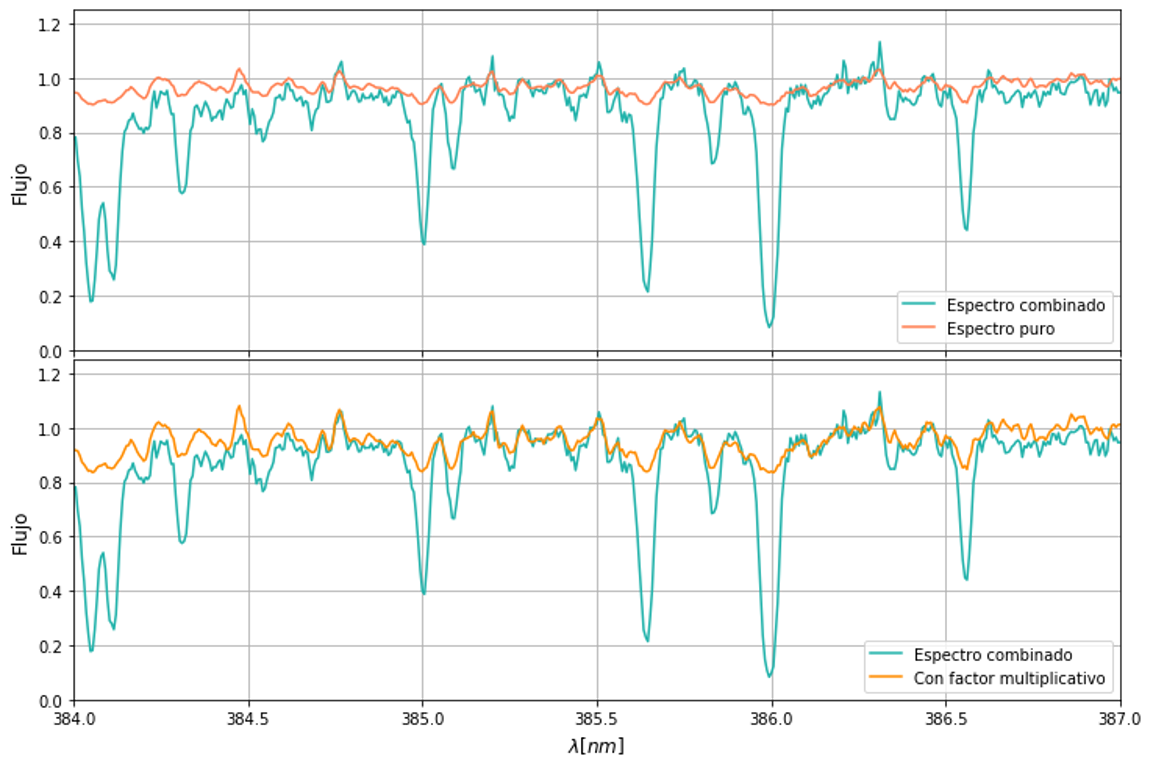
\includegraphics[width=1\linewidth]{Gaficas/factor_mult.png}
    \caption{Ventana espectral de ejemplo, en la cual se observa la diferencia del espectro en flujo del espectro puro al tener en cuenta un factor antes de la sustracción de líneas cromosféricas.}
    \label{fig:ej_sus}
\end{figure}


Debido a que el espectro puro no tiene un continuo espectral en un solo valor, como se mencionó en la sección \ref{sec:normalizacion}, es necesario crear continuos locales o pseudocontinuos al rededor de las líneas que se van a analizar para tener como referencia. Una vez revisada y aprobada la sustracción, como se observa en la figura \ref{fig:sustracciones}, para las dos fechas durante el eclipse parcial, se observa que la diferencia entre estas es sobre todo la cantidad de líneas que se aprecian junto a sus variaciones en ancho y profundidad. Por lo que es necesario identificar las líneas de absorción presentes, que como ya mencionamos anteriormente solo se forman en la cromósfera. Para esto se tomó como referencia una lista de líneas publicada en \citep{kps9} para este mismo sistema en el rango de 3650 - 4600 \r{A}. De esta lista obtenemos la longitud de onda y el elemento con la que se relacionan, lo cual es muy importante para posteriormente obtener los datos atómicos correspondientes a estas lineas.

\begin{figure}[h]
    \centering
    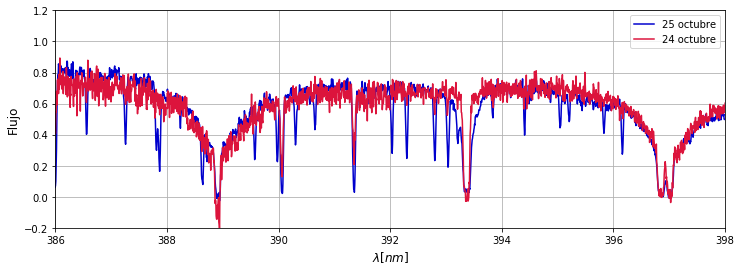
\includegraphics[width=1\linewidth]{Gaficas/sustracciones.png}
    \caption{Espectro de líneas cromosféricas, sustraído para ambas fechas del eclipse parcial.}
    \label{fig:sustracciones}
\end{figure}

Una vez identificadas todas las líneas de absorción que se encuentran en el espectro (196 aproximadamente), se escoge con cuales de estas se harán los cálculos de densidad de masa columnar, por lo tanto es necesario poner algunas restricciones:

\begin{itemize}
    \item[1)] Deben estar dentro de los límites útiles, lo suficientemente fuertes para ofrecer una medición precisa, pero sin estar saturadas, es decir que su intensidad de absorción se extienda hasta cero o por debajo de este umbral,  como para perder información relevante respecto a la densidad. Tampoco deben ser tan débiles como para confundirse con imperfecciones de la sustracción. Algunos ejemplos de estos casos se observan en la figura \ref{fig:example_lines} a y c, respectivamente.
    
    \item[2)] Deben ser líneas sin mezclar. A medida que la línea de visión de la estrella B atraviesa capas cromosféricas sucesivamente más profundas, dan lugar a un espectro de líneas de absorción cada vez más rico; así que en algunos casos estas pueden estar mal resueltas debido a la resolución del espectrógrafo, un ejemplo de esto lo podemos ver en la figura \ref{fig:example_lines} b, donde se observa la combinación de una línea de Fe I, junto con una de Ti II , por lo que no es certero identificar dónde comienza o termina cada una.
    
    \item[3)] Se debe encontrar una concordancia con la lista de valores atómicos que provee el repositorio VALD \citep{ryabchikova1997vienna}.
\end{itemize}

\begin{figure}
    \centering
    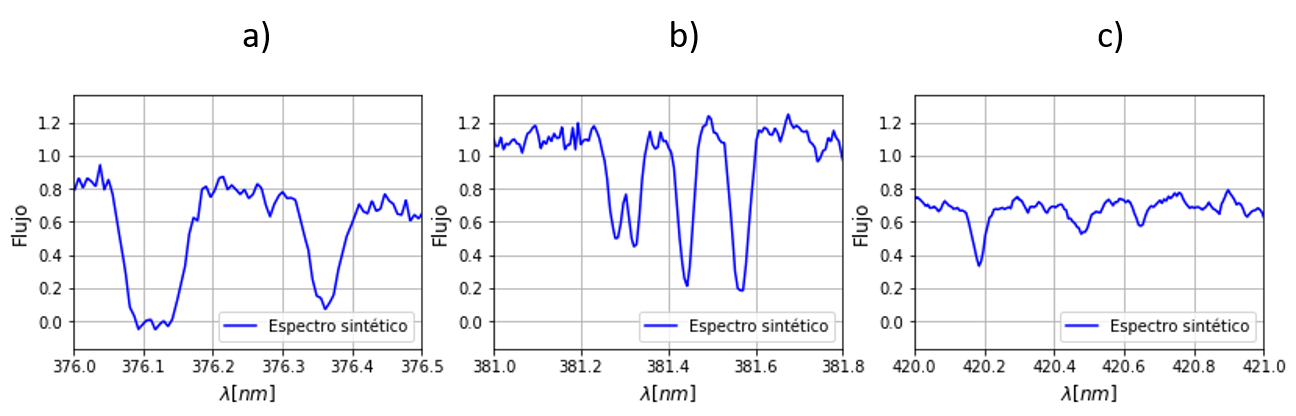
\includegraphics[width=1\linewidth]{Gaficas/examples_lines.png}
    \caption{Algunos tipos de líneas en el espectro sustraído: a) Líneas saturadas b) Líneas que no se pueden analizar individualmente c) Líneas débiles.}
    \label{fig:example_lines}
\end{figure}

Por otro lado, luego de aplicar estas restricciones nos quedamos con 100 líneas de absorción cromosférica, el día 25 octubre (altura $\num{4.39e6}$ km) y con 41 líneas del día 24 octubre (altura $\num{1.02e7}$ km). Como con estas líneas se calculan los anchos equivalentes, cada una aporta un punto a la gráfica de las curvas de crecimiento, es necesario hacerlo con elementos que tengan gran cantidad de líneas y así hacer ajustes racionales. Por lo tanto, se escogen los elementos de Fe I (Hierro neutro) y Ti II  (Titanio una vez ionizado)\footnote{Esta notación de números romanos es utilizada en astronomía, en importante no confundir con la notación química donde $Fe^{+}$ indica una vez ionizado y $Fe^{++}$ es dos veces ionizado} son los elementos con mayor cantidad de líneas funcionales en ambas fechas, 21 de Ti II y 25 de Fe I el 25 de octubre y 10 de Ti II, 9 de Fe I el 24 de octubre. 

A cada una de estas líneas se les registro en dos archivos diferentes, uno para cada fecha, las líneas empleadas se ven en las tablas \ref{table:lines} y \ref{table:lines2}. Donde \textit{wave\_peak} es la longitud de onda del pico central; \textit{wave\_base} es el extremo izquierdo, donde comienza la línea y \textit{wave\_top} es el extremo derecho donde termina la línea, siguiendo la notación que usa el programa iSpec. Estos extremos son calculados con un código creado que identifica las variaciones del continuo, y con un filtro pasa bandas, donde se definía un \textit{threshold} a partir del cual se consideraba una línea que cumplía con el primer item de las restricciones. Los otros dos items, se terminaron de completar con revisiones exhaustivas individuales de cada línea.


\chapter{Curvas de Crecimiento}\label{cap:Resultados}

Como se explicó en la sección \ref{CoG}, las curvas de crecimiento (GoC\footnote{Por sus siglas por su nombre en inglés Growth of Curve}) son un método para calcular la densidad de masa columnar. Una ventaja de las GoC es que son independientes de la resolución del espectrógrafo y del SNR que tengan los datos, ya que el ancho equivalente no depende de estos dos parámetros mencionados antes. En este capítulo se explica cómo se obtienen las curvas de crecimiento de cada fecha del eclipse parcial asociadas a las líneas explicadas en el capítulo anterior. Inicialmente se calculan los anchos equivalentes de cada una de las líneas por elemento, y se relacionan con los datos atómicos asociados a cada una de ellas, es decir, con la probabilidad de transición dada por el fuerza del oscilador y las energías de excitación entre los niveles transitorios.


\section{Anchos equivalentes y datos atómicos}

Para calcular los anchos equivalentes, inicialmente se usó la herramienta que tiene el código de iSpec (\texttt{fit lines determine ew and crossmatch with atomic data}), haciendo variaciones en el tipo de perfil que se ajusta  a la línea: Gauss o Voigt, lo cual mostraba comportamientos similares pero con valores diferentes, causando discrepancia en los resultados. Además, este código solo se podía usar para espectros con una normalización del continuo situado en la unidad, pero en estos espectros no se pudo obtener debido a lo explicado en la sección \ref{sec:normalizacion}. Dada estas situaciones se aprecia que se pueden estar introduciendo errores, evidenciados en la alta dispersión de los datos.


Como resultado de estas pruebas, fue necesario crear un código que fuese recursivo e hiciera el procedimiento de calcular los anchos equivalentes de todas las líneas de un mismo elemento, mencionadas en las tablas  \ref{table:lines} y \ref{table:lines2}. Adicionalmente, este código extrae los valores atómicos del repositorio de VALD y los asocia a su línea correspondiente. Su instalación y manual de uso están disponibles en un repositorio de Github  \footnote{\url{https://github.com/ntlucia/Tesis_Estrellas_binarias/tree/master/Scripts/Growth_curve}} y está descrito en el apéndice \ref{apendiceCoG}.

Como inputs del código se tienen:
\begin{itemize}
    \item Archivo config.yaml, para editar la dirección de los archivos necesarios:
    \begin{itemize}
        \item Líneas teóricas de la cromósfera: contiene la información de la tabla \ref{table:lines} ó \ref{table:lines2}.
        \item Lista de líneas atómicas provista por VALD: contiene muchos parámetros, pero los que empleamos en este proyecto son: longitud onda, elemento, loggf, energías de los dos niveles transitorios (\textit{wave\_nm, element, loggf, lower\_state\_eV, upper\_state\_eV} respectivamente)
        \item Espectro a analizar, en este caso las dos sustracciones, este contiene: longitud de onda, flujo y error de flujo (\textit{wave\_obs, flux, err respectivamente})
    \end{itemize}
    
    \item Elemento que se va a analizar, con su respectiva ionización, escrito como \textit{string}, por ejemplo: ``Ti 2'', ``Fe 1''.
\end{itemize}

Como output, el código entrega un archivo \texttt{dataFrame} listo para generar la curva de crecimiento, el cual contiene:

\begin{itemize}
    \item Pico de la línea, [nm] (\textit{wave\_peak})
    \item Extremo derecho, donde comienza la línea, [nm] (\textit{wave\_base})
    \item Extremo izquierdo, donde termina la línea [nm] (\textit{wave\_top})
    \item Elemento que se está analizando, si es el mismo quiere decir que hizo el \textit{match} con la lista de datos atómicos (\textit{note})
    \item Flujo asociado al pico de la línea (\textit{flux})
    \item Fuerza del oscilador, probabilidad de transición (\textit{loggf})
    \item Energía del nivel inferior en la transición (\textit{lower\_state\_eV})
    \item Energía del nivel superior en la transición (\textit{upper\_state\_eV})
    \item Ancho equivalente de cada línea (\textit{EWR})
    \item Error relacionado al ancho equivalente (\textit{errEWR})
    \item Error relacionado con el flujo del pico de la línea (\textit{error\_f})
\end{itemize}

Inicialmente el \textit{script} separa los datos del elemento que se va a analizar, tanto de la lista de líneas teóricas como de la lista de VALD. Luego, de acuerdo a la longitud de onda del pico de la línea, las las líneas teóricas son emparejadas con los datos atómicos de las transiciones espectroscópicas. Se sigue este orden, debido a que la lista VALD contiene información de más de setecientas mil transiciones (731,377), por lo tanto, para reducir tiempo de computo es mejor reducir esta lista desde el inicio.

% El error instrumental del espectrógrafo HEROS es variable con la longitud de onda. Así que debes decir que ese es el error pero definiendo alrededor de qué longitud de onda. Ver las ecuaciones del informe técnico en la página de tigre

Como solo se tienen los picos y extremos de las líneas como valores teóricos, es necesario asociar los valores reales que se tienen en el espectro con su respectiva cantidad de decimales y posibles variaciones en longitud de onda, eso se logra con la rutina \texttt{nsmallest} de pandas en python. Una vez conocidos los valores reales de las línea, es posible el cálculo de anchos equivalentes, para esto es necesario primero encontrar el continuo local para cada línea. El continuo lo obtenemos con los datos al rededor de la línea,
asumiendo un ancho del continuo de 0.06 nm a la derecha del extremo base y 0.06 nm a la izquierda del extremo superior. Estos valores se corresponden con el doble en un factor adicional del error instrumental del espectrógrafo, como se indica en la figura \ref{fig:continuo}. Entonces ese continuo local corresponde al promedio de los valores de flujo en el rango mencionado anteriormente.

\begin{figure}[h]
    \centering
    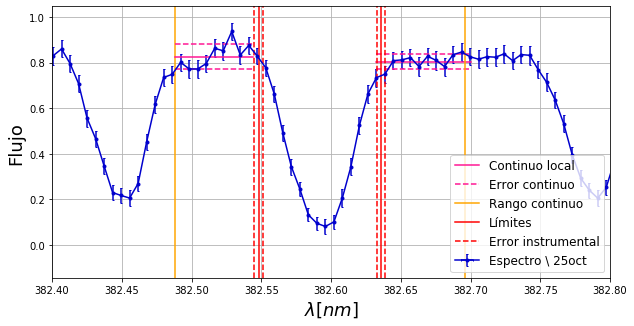
\includegraphics[width=1\linewidth]{Gaficas/continuo.png}
    \caption{Cálculo del continuo local, con la respectiva propagación de errores.}
    \label{fig:continuo}
\end{figure}

Ahora, como se observa en la figura \ref{fig:anchoeq_} procedemos al cálculo de las áreas necesarias para obtener el ancho equivalente según la teoría descrita en la sección \ref{CoG}. Calculamos la integral de la datos que conforman la línea y el área bajo el continuo en el rango de los límites de la línea. Ahora, la resta de estas dos es el área dentro de la línea, que debe ser igual a la de un rectángulo de la altura del continuo y su ancho es el \textit{ancho equivalente} asociado a la línea. Por último, como la curva de crecimiento es adimencional en el \textit{eje y}, se divide el ancho equivalente entre la longitud de onda del pico de la línea y se obtiene el logaritmo base 10 de esta cantidad.

\begin{figure}[h]
    \centering
    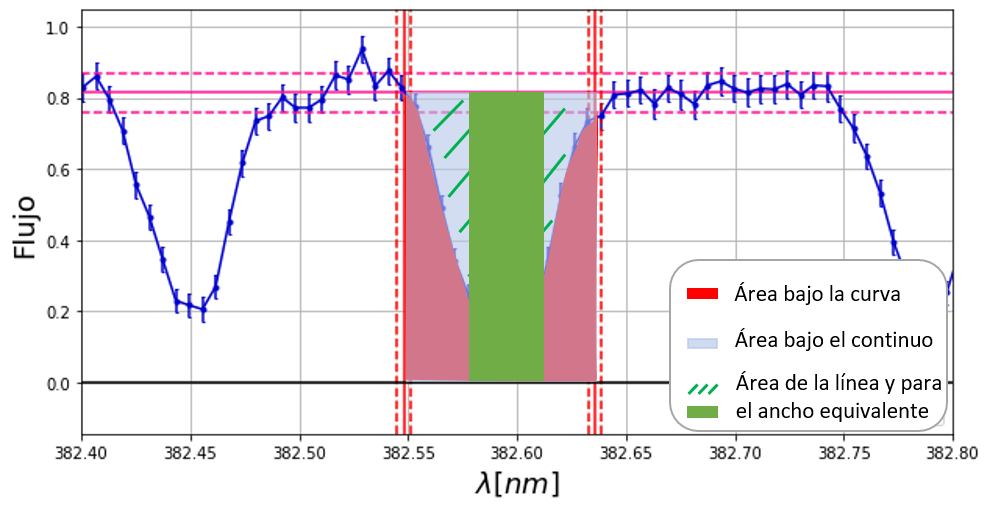
\includegraphics[width=1\linewidth]{Gaficas/ancho_eq.png}
    \caption{Representación del cálculo de ancho equivalente.}
    \label{fig:anchoeq_}
\end{figure}

Este proceso se repite de manera iterativa, para todas las líneas de un mismo elemento que tiene el espectro. Cabe resaltar, que se hace la respectiva propagación de errores teniendo en cuenta los errores en el flujo de cada dato y de la longitud de onda, dados por el espectrógrafo, y errores incluidos debido a la selección del continuo local, como se refleja en la figura \ref{fig:continuo}. Por último, se agregan estos valores de ancho equivalente a la lista completa que posee los datos atómicos asociados a cada línea, obteniendo como último la descripción del output del código (el código se encuentra en el apéndice \ref{apendiceCoG}).


\begin{comment}
\begin{table}[h]
\centering
\resizebox{16cm}{!}{
\begin{tabular}{|c|c|c|c|c|c|c|c|c|c|c|c|}
\hline
\textbf{wave\_peak} & \textbf{wave\_base} & \textbf{wave\_top} & \textbf{note} & \textbf{flux} & \textbf{loggf} & \textbf{lower\_state\_eV} & \textbf{upper\_state\_eV} & \textbf{EW} & \textbf{EWR} & \textbf{error\_f} & \textbf{errEWR} \\ \hline
390.063767          & 389.996654          & 390.106476         & Ti 2          & 0.129236      & -0.29          & 1.131                     & 4.308                     & 0.049013    & -3.900827    & 0.007739          & 0.016607        \\ \hline
391.351118          & 391.296207          & 391.399927         & Ti 2          & 0.207386      & -0.36          & 1.116                     & 4.283                     & 0.039436    & -3.996678    & 0.006613          & 0.019102        \\ \hline
\end{tabular}
}
\end{table}
\end{comment}



\section{Curvas de crecimiento observacionales y empíricas}

Para la curvas de crecimiento observacionales tomamos los datos recolectados por el código explicado en la sección anterior y graficamos $log(W_{\lambda}/\lambda)$ en el \textit{eje y} y $log(gf)$ en el \textit{eje x}, continuando con la misma nomenclatura de estudios anteriores \citep{kps1O}. Se obtuvieron cuatro curvas de crecimiento observacionales, dos de ellas para el titanio una vez ionizado (Ti II), una para cada fecha que se tenía durante el eclipse parcial y las otras dos para el hierro neutro (Fe I), también de estas fechas. Estos elementos también se han analizado antes para el sistema $\zeta$ Aurigae. Estas gráficas se aprecian en la figura \ref{fig:GoC_obs}, donde se observa un comportamiento lineal debido a que se están analizando líneas de tipo fuerte y no saturadas o con \textit{damping}\footnote{líneas con \textit{alas} pronunciadas, que se amortiguan con el continuo, debido a disipación de energía}. Además, también se aprecia a simple vista que el comportamiento de las dos fechas no tiene mucha variación.


\begin{figure}[h]
    \centering
    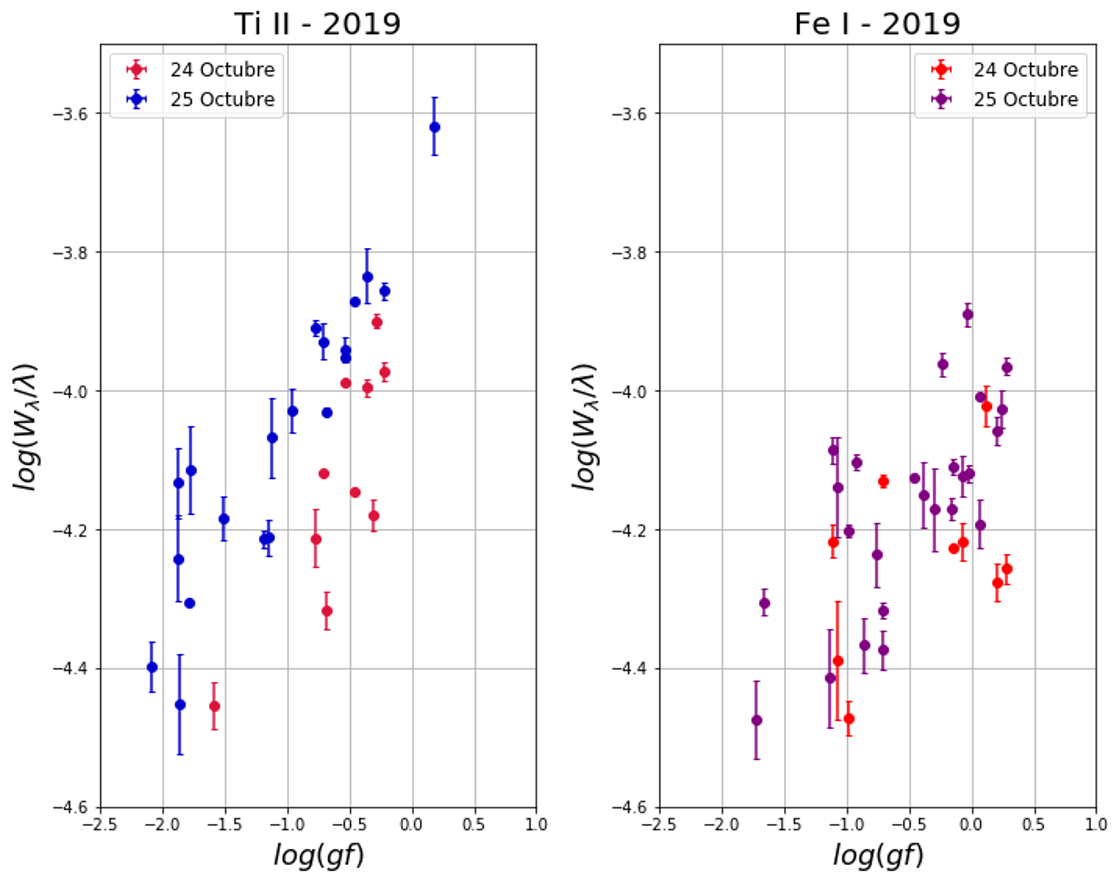
\includegraphics[width=1\linewidth]{Gaficas/GoC_obs.png}
    \caption{Curvas de crecimiento observacionales para los elementos de Ti II y Fe I respectivamente, del eclipse $\zeta$ Aurigae de 2019.}
    \label{fig:GoC_obs}
\end{figure}



\noindent De acuerdo a los datos de las curvas de crecimiento observacionales, se procede a contrastar con el comportamiento de valores teóricos asociados a cada una de las transiciones de las líneas de absorción que aportan a la curva. Partimos teniendo en cuenta que se considera absorción pura, como se indicó en la sección \ref{sec:densidad_masa,} y que teóricamente cada línea se modela como un perfil de gaussiano de la forma:

\begin{equation*}
    I = I_0 exp\left(-A_ie^{-(\Delta\lambda/\Delta\lambda_D)^2}\right).
\end{equation*}

Donde $\Delta\lambda_D$ es el corrimiento doppler, $\Delta\lambda$ el ensanchamiento debido a otros fenómenos físicos, $I_0$ la intensidad del continuo y el término $A_i$ es la ecuación de Saha (ec \ref{saha}), que por términos de comprensión lectora se reescribe en la ecuación \ref{saha_2}. Es en esta fórmula donde se tienen en cuenta los factores de la profundidad óptica que afectan el ensanchamiento de la línea

\begin{equation}
    A_{i}=\frac{\pi e^{2}}{m_{e} c^{2}} \frac{\lambda \cdot c}{v \sqrt{\pi}} g f \frac{N_{i}^{i o n}}{Z(T)} \cdot \exp \left(-E_{i} / k T_{exc}\right).
    \label{saha_2}
\end{equation}

En consecuencia, se obtienen los valores teóricos del ancho equivalente, como lo describe la ecuación \ref{ec:ancho-eq}, teniendo en cuenta los factores de ensanchamiento que pueden afectar a la línea

\begin{equation}
    W = \int \frac{I_0 - I}{I_0}d \lambda = \int \left[1 - exp(-A_i e^{-(\Delta\lambda/\Delta\lambda_D)^2)}\right] d\lambda.
    \label{ec:ancho-eq}
\end{equation}

Dentro de estos factores, se tienen en cuenta $T_{exc} = 5000$ K, de acuerdo a los análisis presentados en \citet{kps1O} para estos mismos elementos. Se tomaron los cálculos  de $N_i^{ion}$ y $Z(T)$ de este mismo estudio, donde tenemos que $Z(T=5000K) = 53.5$ para el Ti II y  $Z(T=5000K) = 27.0$ para el Fe I, y además los valores de $E_i$ y $fg$ del repositorio VALD. 

Además uno de los factores más relevantes es la velocidad de turbulencia, que según \citet{kps1O} se puede tomar su valor en aproximadamente 14 km/s, lo cual es bastante elevado y por lo tanto tiene un efecto de amortiguamiento sobre la curva de crecimiento. Es decir, ahora en la GoC teórica no se observa una línea recta, como en las GoC observacionales (figura \ref{fig:GoC_obs}), sino que ahora se tiene una curvatura en la parte superior, como se observa en la figura \ref{fig:cteoricas_klaus}, que son las curvas de crecimiento teóricas del eclipse de 1987 para estos mismos elementos, tomadas de \citet{kps1O}. Este comportamiento indica que realmente las líneas que a simple vista se consideran fuertes, realmente pueden estar saturadas.



\begin{figure}[h]
    \centering
    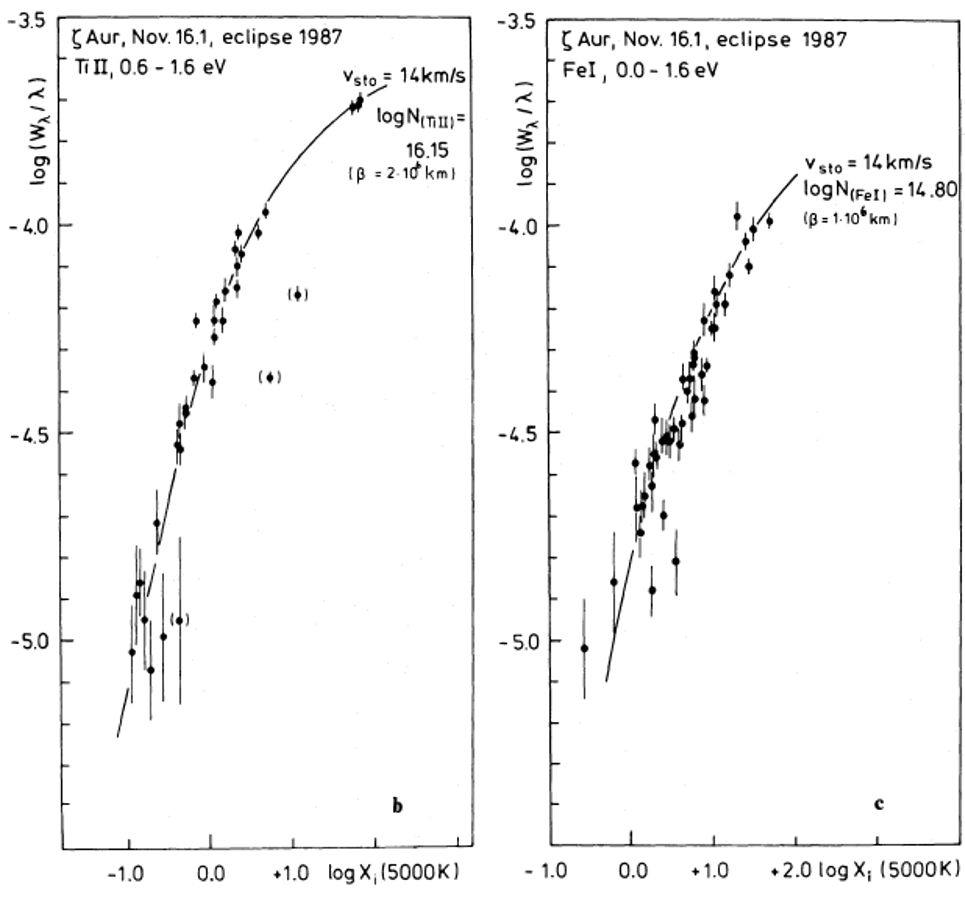
\includegraphics[width=0.8\linewidth]{Gaficas/curvas_klaus.png}
    \caption{Curvas de crecimiento teóricas del eclipse de $\zeta$ Aurigae, eclipse 1987 \citep{kps1O}.}
    \label{fig:cteoricas_klaus}
\end{figure}


En las curvas de crecimiento teóricas (figura \ref{fig:cteoricas_klaus}), se observa que en en el \textit{eje x} se tiene $log(X_i)$, que representa la ecuación \ref{ec:Xi}. La cual contiene los datos atómicos relacionados a la probabilidad de que existan las líneas y todos los parámetros de ensanchamiento a excepción de la densidad de masa columnar

\begin{equation}
    X_{i}= \frac{\pi e^{2}}{vm_{e} c\sqrt{\pi}} g f \lambda \frac{\exp \left(-E_{i} / k T_{exc}\right)}{Z(T_{exc})}.
    \label{ec:Xi}
\end{equation}

De modo que, teniendo en cuenta la ecuación de Saha \ref{saha_2} y $X_i$ (ecuación \ref{ec:Xi}) éstas están relacionas por la densidad de masa columnar, como se observa en la ecuación \ref{ec:sahaXN}

\begin{equation}
    A_i =  N_i^{ion} \cdot X_i.
    \label{ec:sahaXN}
\end{equation}

Por lo tanto, de acuerdo a la curva de crecimiento teórica de $log(X_i)$, es posible obtener el valor $log(N)$ con una nueva curva empírica que ajuste la curva de crecimiento teórica a los datos observacionales. Es decir, teniendo en cuenta propiedades logarítmicas, $log(N\cdot X_i) = log(N) + log(X_i)$, entonces $log(N)$ es un factor aditivo generado al comparar la curva de crecimiento teórica y observacional.

En la figura \ref{fig:GoC_teo} observamos la curva de crecimiento empírica, resultado de la comparación entre la curva teórica y observacional. Con la cual se obtuvieron los valores de densidad de masa columnar $log(N)$ asociados a cada elemento en cada fecha, registrados en la tabla \ref{tabla:dens_colum}. En la figura \ref{fig:GoC_teo} también se aprecia que las curvas de Ti II son mucho más confiables, ya que conocemos que no hay líneas de este tipo en la fotósfera de la estrella.



\begin{figure}
    \centering
    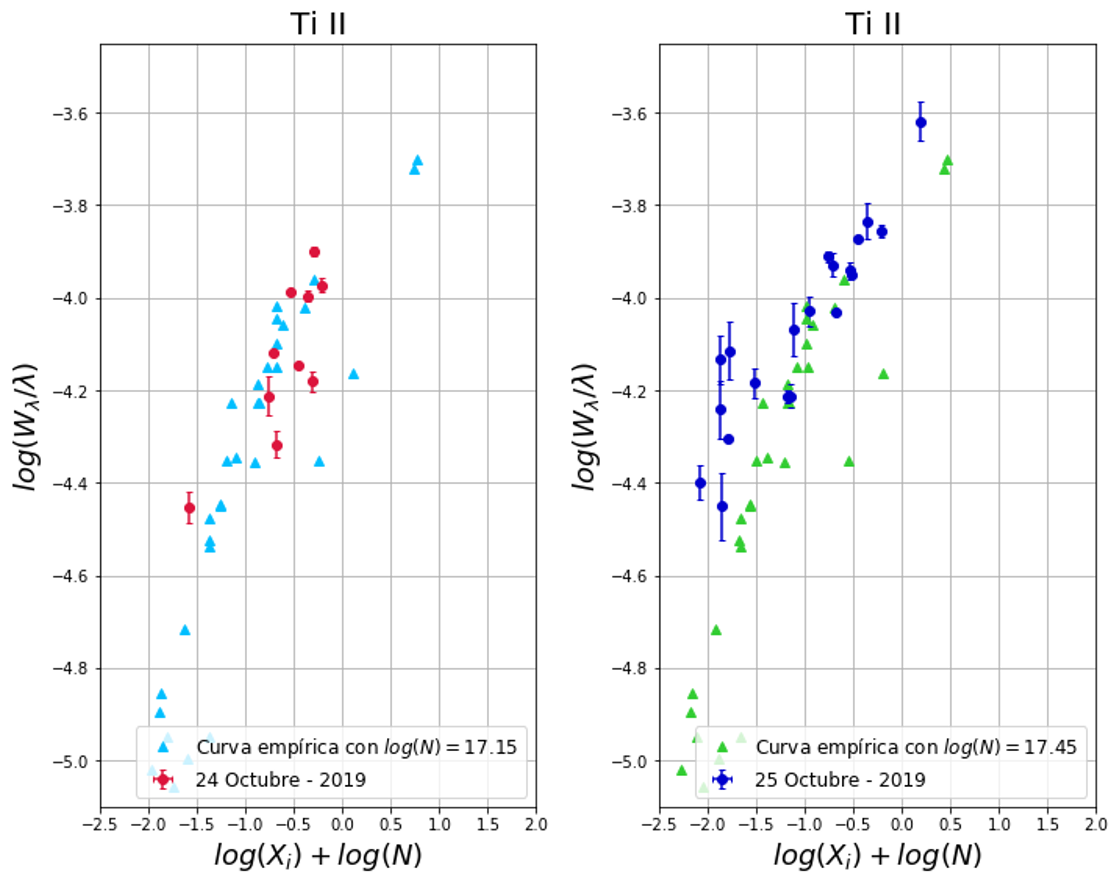
\includegraphics[width=0.8\linewidth]{Gaficas/curva_teoTi2.png}
    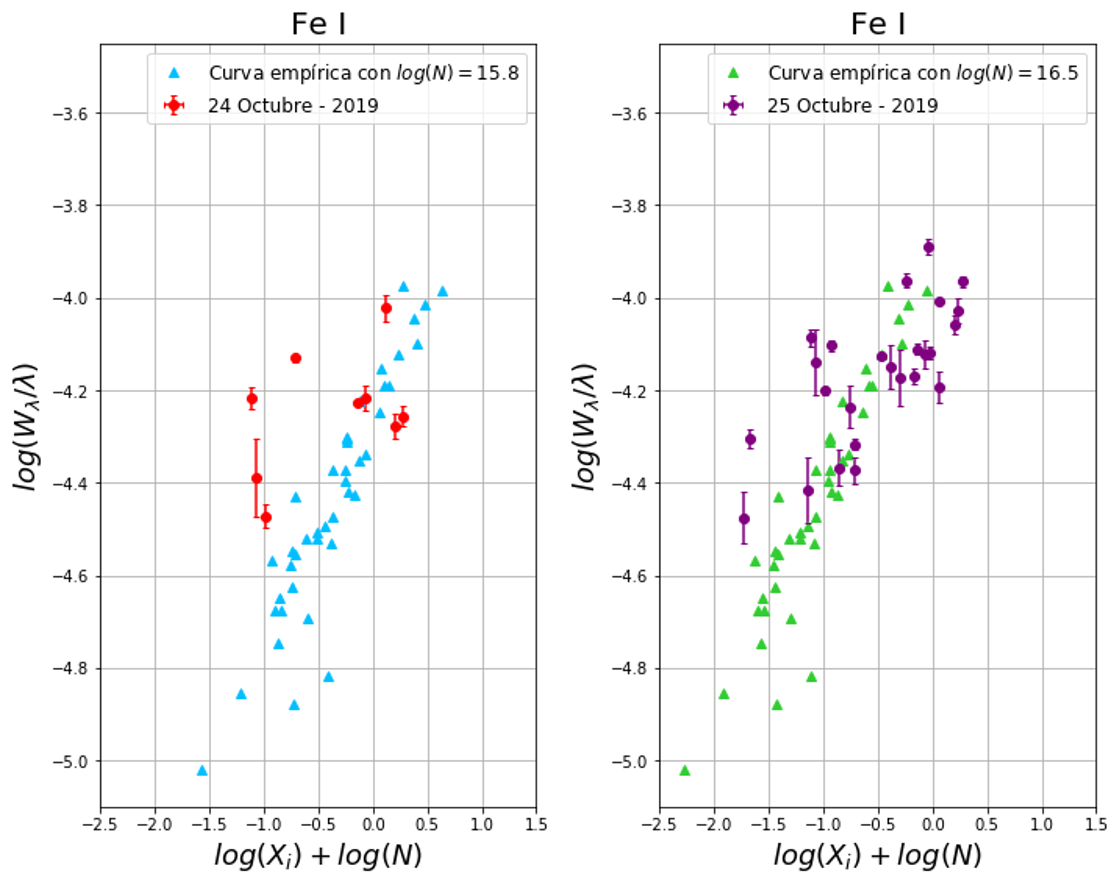
\includegraphics[width=0.8\linewidth]{Gaficas/curva_teoFe1.png}
    \caption{Curva de crecimiento empírica y observacional para los elementos de Ti II y Fe I, respectivamente. Del eclipse $\zeta$ Aurigae de 2019.}
    \label{fig:GoC_teo}
\end{figure}

\begin{table}[h]
\centering
\begin{tabular}{|c|c|c|}
\hline
                & \begin{tabular}[c]{@{}c@{}}24 Octubre\\ $h = \num{1.02e7}$ km\end{tabular} & \begin{tabular}[c]{@{}c@{}}25 Octubre\\ $h=\num{4.39e6}$ km\end{tabular} \\ \hline
$log(N_{TiII})$ & $17.15$                                                                    & $17.45$                                                                  \\ \hline
$log(N_{FeI})$  & $15.8$                                                                     & $16.5$                                                                   \\ \hline
\end{tabular}
\caption{Densidades de masa columnar del eclipse $\zeta$ Aurigae, 2019.}
\label{tabla:dens_colum}
\end{table}
\vspace{3mm}

Llegados a este punto, es posible comparar como varía la densidad de masa columnar de cada elemento con respecto a la altura proyectada calculada en la sección \ref{sec:fotometria}. Estas variaciones se observan en la figura \ref{fig:dens_alt1}, donde se aprecia que para el caso del Ti II, las variaciones de densidad entre ambas fechas no son tan pronunciadas, mientras que para el hierro Fe I se observa una diferencia mayor entre las dos fechas. Con esto se corrobora lo que se observaba en las curvas de crecimiento observacionales, que su comportamiento en las dos fechas era similar.

\begin{figure}[h]
    \centering
    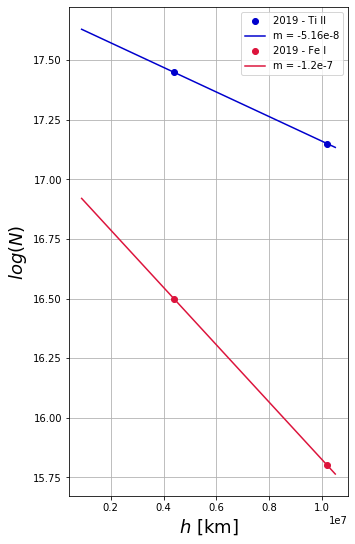
\includegraphics[width=0.5\linewidth]{Gaficas/altura_dens_.png}
    \caption{Densidades empíricas en la cromosfera baja de $\zeta$ Aurigae en la entrada del eclipse de 2019.}
    \label{fig:dens_alt1}
\end{figure}


\section{Discusión}\label{discusion}

En esta investigación se tuvieron en cuenta los parámetros de eclipses anteriores para hacer una correcta comparación, que solo fuese afectada por variaciones en densidad de masa columnar y no debido a parámetros externos. 

Por consiguiente, uno de estos parámetros es la velocidad tangencial relativa, como se indicó en la sección \ref{sec:fotometria}, que es la misma usada en \citet{kps1O}. Pero en el caso de comparar con un eclipse aún más antiguo (1947-1948) \citep{wilson1954chromospheric}, en esta época no se conocía con certeza la fracción de masa de las estrellas, ni la trayectoria de orbita de las estrellas. Lo cual afecta el cálculo de velocidad transversal y por ende las alturas proyectadas en las fechas del ingreso y egreso. En este caso, se hizo un ajuste de un factor constante, para  obtener las alturas de proyectadas verdaderas partiendo de las registradas por \citet{wilson1954chromospheric}, ya que se habían calculado con $v_{tan} =$ 46.43 y ahora se conoce que $v_{tan} =$ 65.00.


Por otro lado, del artículo \cite{kps1O} no solo se conoce la densidad de masa columnar para diferentes alturas, sino que también se tienen los datos de ancho equivalente y $log(gf)$ empleados para generar las curvas de crecimiento observacionales. Así que, de acuerdo a la figura \ref{fig:Ti2Klaus} vemos que éstas tienen el mismo comportamiento lineal que se observa en las figuras \ref{fig:GoC_obs}, sin embargo su variación de la pendiente entre las dos fechas es mucho mayor, lo cual inicialmente indica que el gradiente de densidad de masa entre las dos fechas es también es mayor.

\begin{figure}[h]
    \centering
    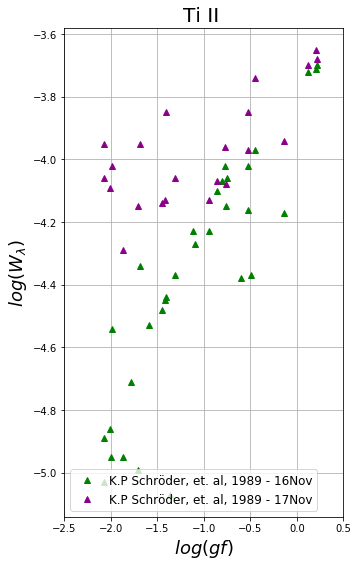
\includegraphics[width=0.5\linewidth]{Gaficas/Ti2Klaus.png}
    \caption{Curva de crecimiento observacional Ti II del eclipse $\zeta$ Aurigae de 1987}
    \label{fig:Ti2Klaus}
\end{figure}

Adicionalmente, en la GoC observacional de FeI en el eclipse de 2019 (figura \ref{fig:GoC_obs}) se observa una gran dispersión en los datos, para las dos fechas del ingreso. Y ahora, comparando con las curvas de crecimiento de 1987 (figura \ref{fig:curvFe_obs}), nos damos cuenta que también está presente una gran dispersión en los datos de FeI de esa época. Esto se debe a que para alturas de la fotósfera no se alcanzan las energías de ionización de los elementos, $E_i = 7.9$ [eV] del hierro y $E_i = 6.11$ [eV] del titanio. Es decir, en esta zona son más probables las líneas de elementos neutros como el Fe I. Mientras que en la cromósfera a medida que aumenta la altura y la temperatura, se alcanzan estados de ionización, en este caso primero del Ti II y luego del Fe I.

Por lo tanto, para el tipo de líneas de elementos neutros como el Fe I, el proceso de sustracción como se indica en la sección \ref{sec:sustraccion}, se convierte en un procedimiento mucho más tedioso, con el cual se pueda asegurar que en la curva de crecimiento solo se estén analizando líneas cromosféricas. Sin embargo, este problema de sustracción espectral de componentes estelares siempre se ha tenido, y en la actualidad se sigue estudiando y se siguen diseñando procedimientos para lograr que las sustracciones no contengan remanentes de la fotósfera. De modo que cuando hay combinación de líneas de la cromósfera y fotósfera, no es posible obtener resultados igual de concluyentes que en el caso de que solo se tenga en cuenta la cromósfera.

\begin{figure}[h]
    \centering
    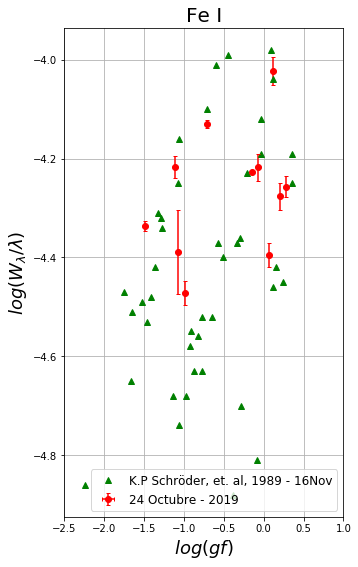
\includegraphics[width=0.5\linewidth]{Gaficas/Fe_1987.png}
    \caption{Comparación de la dispersión en las curvas de crecimiento observacionales del Fe I del eclipse de 2019 y eclipse de 1987.}
    \label{fig:curvFe_obs}
\end{figure}

En el caso del Ti II, esta dispersión no se observa debido ya que a alturas de la fotósfera no se ha alcanzado la energía de ionización de este elemento. Por consiguiente, las precauciones en la sustracción no son tantas para evitar remanentes fotosféricos para estas líneas, ya que son muy poco probables.

Con esto claro, ahora es posible no solo comparar las curvas de crecimiento, sino también analizar el comportamiento de la densidad de masa columnar con respecto a la altura. Los valores obtenidos en este proyecto se pueden contrastar con los eclipses de 1987 y 1047-1948 estudiados en investigaciones anteriores registradas en \citet{kps1O} y \citet{wilson1954chromospheric}, respectivamente. Con estos datos generamos la gráfica de la figura \ref{fig:den_alt_compara}, donde observamos la variación de la densidad de masa columnar del Ti II y Fe I para diferentes alturas de la atmósfera estelar. 

\vspace{20mm}

Cabe resaltar, que en esta gráfica para el 2019 solo tenemos dos puntos, debido a condiciones climáticas del momento en que se tomaron los datos del eclipse, al igual que en el caso del eclipse de 1987, donde solo se pudieron tomar espectros de dos fechas durante el eclipse parcial. Sin embargo se conoce de acuerdo a la literatura \citep{vernazza1973structure} que el comportamiento de la densidad a alturas cromosféricas tiene un comportamiento lineal.


En la figura \ref{fig:den_alt_compara} también se observa que las variaciones de densidad respecto a la altura del Fe I son mayores que para el Ti II, tanto en nuestros resultados como para estudios anteriores. Este comportamiento se debe a que se está comparando un elemento neutro y uno ionizado. A alturas mayores, es poco probable tener elementos neutros, la mayor probabilidad está en tener elementos con estado de ionización dominante. Por lo tanto, a medida que aumenta la altura, y por ende la temperatura se van alcanzando las energías de ionización los elementos, por lo que la fracción de Fe I disminuye y comienza a haber mayor presencia de Fe II (hierro una vez ionizado). Por lo tanto, de acuerdo con la definición de \textit{densidad de masa columnar}, si la fracción de átomos de una misma especie disminuye, la densidad también, que es lo que sucede con el Fe I. Para el caso del Ti II no disminuye la fracción de átomos, ya que este desde bajas alturas de la cromósfera ya se encuentra en su primer estado excitado y la variación de temperatura a alturas mayores no lo lleva a un estado superior de excitación.


\begin{figure}[h]
    \centering
    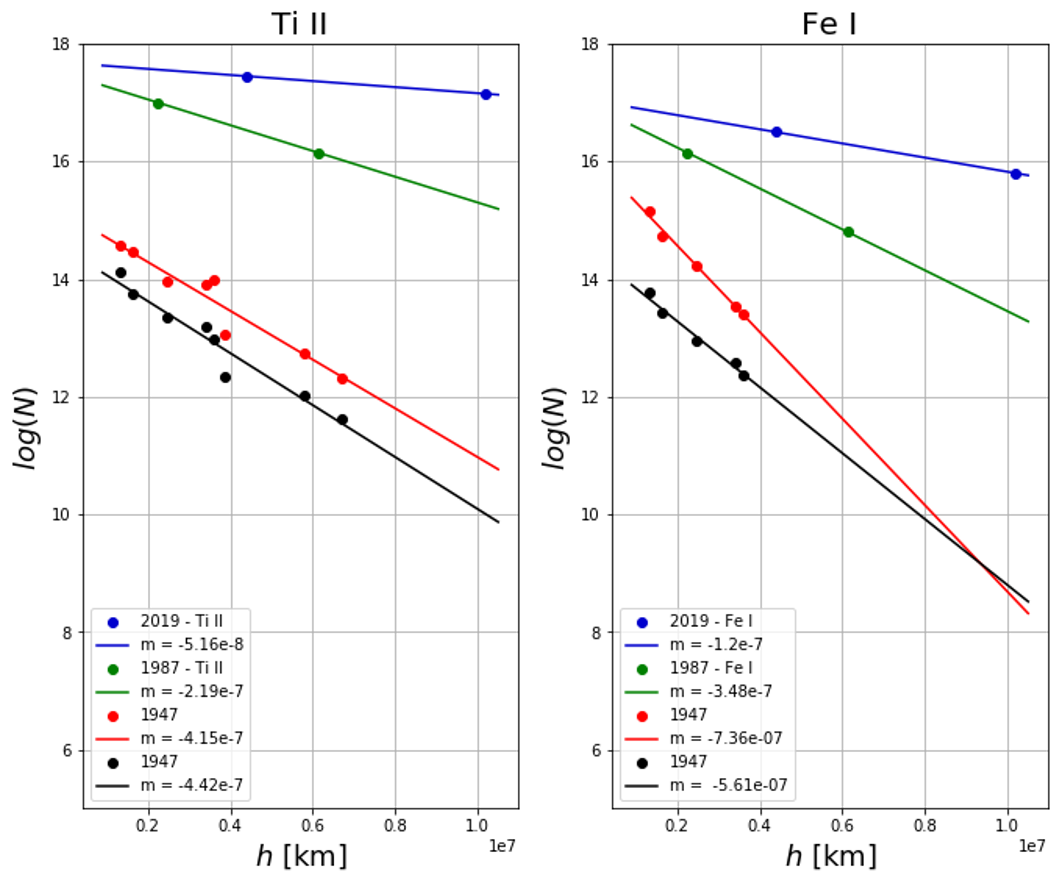
\includegraphics[width=1\linewidth]{Gaficas/alt_den.png}
    \caption{Densidades de masa columnar empíricas en la cromósfera en el ingreso de los eclipse de $\zeta$ Aurigae de 1947, 1987 y 2019 para los elementos de Ti II y Fe I.}
    \label{fig:den_alt_compara}
\end{figure}


Finalmente, observamos que tanto las densidades de columna, como su \textit{pressure scale height}\footnote{Es la distancia vertical sobre la cual la presión atmosférica cae en un factor $\exp$} (ecuación \ref{scale height}) o gradiente de densidad son notablemente diferentes de los valores obtenidos en \citep{kps1O} y \citep{wilson1954chromospheric}. Aunque el comportamiento de estos es el mismo, lo que esperábamos, a medida que aumente la altura atmosférica disminuye la densidad de masa columnar. Las grandes variaciones entre los tres eclipses confirma que la cromosfera de la supergigante $\zeta$ Aur A es muy variable.

Inicialmente, la fotósfera se modela como un equilibro hidrostático con gran influencia de la temperatura y se hacen aproximaciones de gas ideal tal que el gradiente de presión se puede escribir como en la ecuación \ref{grad_presion}

\begin{equation}
    \frac{d P}{d h}=-g N(h) =  -g \frac{P(h)}{kT}
    \label{grad_presion}.
\end{equation}

La solución a esta ecuación diferencial, asumiendo una temperatura constante es de la forma de la ecuación \ref{sol_P}

\begin{equation}
    P(h) = P_0 e^{-(h-h_0)/H},
    \label{sol_P}
\end{equation}

donde H, es conocido como \textit{pressure scale height} y queda definido como en la ecuación \ref{scale height}

\begin{equation}
    H \equiv \frac{kT}{gm_H}.
    \label{scale height}
\end{equation}

Sin embargo, para el caso de la cromósfera, hay una mayor influencia de la turbulencia, por lo que es necesario cambiar la energía térmica por energía cinética ($mv_{tur}^2/2$). De aquí, se obtiene que el \textit{pressure scale height} para una atmósfera turbulenta en equilibrio hidrostático, que está directamente relacionada con el gradiente de densidad, se puede reescribir como en la ecuación \ref{scale height_tur}

\begin{equation}
    H \equiv \frac{v_{tur}^2}{2g}.
    \label{scale height_tur}
\end{equation}

Por lo tanto, debido a que los gradientes de densidad varían con la altura y no pueden explicarse por cambios lentos de un equilibrio hidrostático, a menos de que se garantizara $v_{tur}$ constante, lo cual no es posible, ya que se observa que las curvas de crecimiento, cambian día a día durante el eclipse parcial. Esto indica que $v_{tur}$ debe ser variable y/o no existe un equilibrio en la parte alta de la cromósfera. Cabe resaltar entonces que no se pueden hacer aproximaciones hidrostáticas, ya que se tienen procesos altamente dinámicos, lo cual confirma conclusiones similares hechas actualmente en la literatura \citep{ayres2019stellar}.

\begin{comment}
\begin{equation}
    N (h) = N_0 e^{-E(h)/kT}
    \label{densidad_prob}
\end{equation}

De la ecuación \ref{densidad_prob}, entonces se puede deducir que el gradiente de densidad se puede escribir como

\begin{equation}
    \nabla N = -\frac{N}{kT} \frac{dE(h)}{dh} = kT\nabla P 
\end{equation}

\begin{equation}
    P = \rho(h) \frac{v_{tur}^2}{2}
\end{equation}

\end{comment}



%%%%%%%%%%%%%%%%%%%%%%
%%%%% CHAPTER 6  %%%%%
%%%%%%%%%%%%%%%%%%%%%%
\chapter{Conclusiones}\label{conclusiones}
%Cambiar el orden de las conclusiones

La conclusión principal generada en el desarrollo de esta tesis es la gran diferencia de los valores de densidad de masa columnar y la variación del \textit{scale height}, o el gradiente de densidad, con respecto a eclipses anteriores. Estas magnitudes siguen el mismo comportamiento en el que la densidad de masa columnar disminuye a medida que aumenta la altura atmosférica. 

Algunas de las diferencias relacionadas con los valores de densidad pueden deberse al desconocimiento de muchos parámetros que se han corregido en la historia del análisis del sistema $\zeta$ Aurigae, como el caso de la $v_{tan}$ para el eclipse de 1947-1948.

Con estos comportamientos en las gráficas de altura proyectada vs densidad de masa columnar se deduce  que la turbulencia atmosférica en la parte alta de la cromósfera tiene un papel muy relevante en el análisis atmosférico. Y su variación a estas escalas de altura debe resultar de procesos altamente dinámicos para poder explicar las variaciones en densidad de masa columnar, que actualmente es una de las características a tener en cuenta para análisis atmosféricos estelares. Ya que estas no pueden explicarse por cambios lentos de un equilibrio hidrostático y solo relacionados a la temperatura.

Adicionalmente, se pudo confirmar que la metodología de curvas de crecimiento es una buena herramienta para el análisis espectral atmosférico y propiedades como la densidad de masa columnar u otros factores que afecten la presencia y el perfil de una línea de absorción de la atmósfera estelar.

También, se confirma la importancia de la sustracción para obtener los espectros de las componentes individuales en sistemas binarios o múltiples, en nuestro caso al obtener la sustracción de la componente $\zeta$ Aur B, tenemos también líneas de la cromósfera de $\zeta$ Aur A. Los errores en la sustracción generan grandes variaciones en la dispersión de datos de la curva de crecimiento y puede ser producir análisis equívocos relacionados con la densidad. A pesar de ser una de las primeras pruebas de sustracción de este tipo para espectros del telescopio TIGRE (tipo Echelle), se superaron los obstáculos obteniendo buenos resultados.

Por último, cabe resaltar que este trabajo sienta un precedente, ya que aporta de manera significativa al estudio de este sistema característico sobre su cromósfera variable y comparando con respecto a periodos de tiempo extendidos, más de 70 años. Además aporta al área del análisis de las cromósferas estelares, que actualmente es un tema de estudio popular en la astrofísica.

\appendix

\chapter{Líneas de absorción empleadas en el análisis}

\begin{longtable}[]{|c|c|c|c|}
\hline
\textbf{wave\_peak}                       & \textbf{wave\_base}             & \textbf{wave\_top}              & \textbf{note}             \\ \hline
\endfirsthead

% aquí añadimos el encabezado del resto de hojas.
\hline
wave\_peak                       & \textbf{wave\_base}             & \textbf{wave\_top}              & \textbf{note}             \\ \hline
\endhead


390.063767                       & 389.996654                      & 390.106476                      & Ti 2                      \\ \hline
391.351118                       & 391.296207                      & 391.399927                      & Ti 2                      \\ \hline
393.205878                       & 393.187575                      & 393.218081                      & Ti 2                      \\ \hline
430.008236                       & 429.977730                      & 430.044843                      & Ti 2                      \\ \hline
439.507784                       & 439.446772                      & 439.550492                      & Ti 2                      \\ \hline
444.388733                       & 444.339923                      & 444.437542                      & Ti 2                      \\ \hline
450.129950                       & 450.093342                      & 450.172658                      & Ti 2                      \\ \hline
454.955988                       & 454.901078                      & 455.010899                      & Ti 2                      \\ \hline
456.359261                       & 456.334856                      & 456.420273                      & Ti 2                      \\ \hline
457.207326                       & 457.146314                      & 457.250034                      & Ti 2                      \\ \hline
382.059010 & 382.004100 & 382.107820 & Fe 1 \\ \hline
386.000377 & 385.963770 & 386.036984 & Fe 1 \\ \hline
386.555585 & 386.543383 & 386.561686 & Fe 1 \\ \hline
388.623887 & 388.605584 & 388.636090 & Fe 1 \\ \hline
404.578490 & 404.554085 & 404.627300 & Fe 1 \\ \hline
429.416421 & 429.337106 & 429.459129 & Fe 1 \\ \hline
430.795289 & 430.740378 & 430.837997 & Fe 1 \\ \hline
438.360761 & 438.318052 & 438.397368 & Fe 1 \\ \hline
440.496176 & 440.422962 & 440.526682 & Fe 1 \\ \hline
\caption{Líneas empleadas para analizar las curvas de crecimiento del 24 Octubre}
\label{table:lines}
\end{longtable}

\begin{longtable}{|r|r|r|r|}
\hline
\textbf{wave\_peak}                       & \textbf{wave\_base}             & \textbf{wave\_top}              & \textbf{note}             \\ \hline
\endfirsthead

% aquí añadimos el encabezado del resto de hojas.
\hline
\textbf{wave\_peak}                       & \textbf{wave\_base}             & \textbf{wave\_top}              & \textbf{note}             \\ \hline
\endhead

\multicolumn{4}{c}{Continua en la página siguiente.}
\endfoot


\multicolumn{4}{c}{ }\\
\endlastfoot

376.116455          & 376.049342          & 376.183568        & Ti 2          \\ \hline
388.233411        & 388.184602          & 388.239512         & Ti 2          \\ \hline
391.357219          & 391.284005          & 391.381624         & Ti 2          \\ \hline
401.247242          & 401.180129          & 401.259445         & Ti 2          \\ \hline
416.158542          & 416.085328          & 416.164644         & Ti 2          \\ \hline
417.354375          & 417.293363          & 417.366577         & Ti 2          \\ \hline
428.794100          & 428.757493          & 428.830707         & Ti 2          \\ \hline
430.014337          & 429.935022          & 430.057046         & Ti 2          \\ \hline
431.295586          & 431.252878          & 431.338295         & Ti 2          \\ \hline
431.503027          & 431.472521          & 431.545735         & Ti 2          \\ \hline
432.088741          & 432.039931          & 432.131449         & Ti 2          \\ \hline
433.803174          & 433.754365          & 433.839781         & Ti 2          \\ \hline
439.507784          & 439.422367          & 439.538290         & Ti 2          \\ \hline
441.789627          & 441.740818          & 441.807931         & Ti 2          \\ \hline
444.394834          & 444.339923          & 444.425340         & Ti 2          \\ \hline
445.059863          & 444.998852          & 445.096471         & Ti 2          \\ \hline
450.142152          & 450.081140          & 450.190961         & Ti 2          \\ \hline
453.400186          & 453.351376          & 453.455096         & Ti 2          \\ \hline
454.955988          & 454.894976          & 455.041405         & Ti 2          \\ \hline
456.383666          & 456.334856          & 456.420273         & Ti 2          \\ \hline
376.384907                                & 376.317794                               & 376.409312                              & Fe 1                               \\ \hline
376.726573                                & 376.659460                               & 376.732674                              & Fe 1                               \\ \hline
378.794876                                & 378.733864                               & 378.800977                              & Fe 1                               \\ \hline
379.508714                                & 379.447703                               & 379.514816                              & Fe 1                               \\ \hline
381.595320                                & 381.522106                               & 381.613624                              & Fe 1                               \\ \hline
382.595915                                & 382.516599                               & 382.644724                              & Fe 1                               \\ \hline
382.791153                                & 382.717939                               & 382.797254                              & Fe 1                               \\ \hline
383.425676                                & 383.364664                               & 383.437879                              & Fe 1                               \\ \hline
385.091300                                & 385.054693                               & 385.127907                              & Fe 1                               \\ \hline
386.555585                                & 386.506775                               & 386.573888                              & Fe 1                               \\ \hline
387.257221                                & 387.177906                               & 387.275525                              & Fe 1                               \\ \hline
388.636090                                & 388.568977                               & 388.642191                              & Fe 1                               \\ \hline
388.715405                                & 388.684899                               & 388.733709                              & Fe 1                               \\ \hline
389.569571                                & 389.508559                               & 389.581773                              & Fe 1                               \\ \hline
390.301714                                & 390.240702                               & 390.332219                              & Fe 1                               \\ \hline
404.590693                                & 404.511377                               & 404.608996                              & Fe 1                               \\ \hline
406.366138                                & 406.286822                               & 406.390543                              & Fe 1                               \\ \hline
407.183697                                & 407.104381                               & 407.195899                              & Fe 1                               \\ \hline
420.209730                                & 420.142617                               & 420.215832                              & Fe 1                               \\ \hline
425.084578                                & 425.017465                               & 425.102882                              & Fe 1                               \\ \hline
427.183387                                & 427.110172                               & 427.195589                              & Fe 1                               \\ \hline
429.416421                                & 429.318802                               & 429.434725                              & Fe 1                               \\ \hline
430.795289                                & 430.728176                               & 430.807492                              & Fe 1                               \\ \hline
438.360761                                & 438.287546                               & 438.379064                              & Fe 1                               \\ \hline
440.483974                                & 440.410759                               & 440.502277                              & Fe 1                               \\ \hline

\caption{Líneas empleadas para analizar las curvas de crecimiento del 25 Octubre.}
\label{table:lines2}
\end{longtable}
\chapter{Growth curve}\label{apendiceCoG}

\begin{comment}
\definecolor{light-gray}{gray}{0.95}

\lstset{
    basicstyle=\footnotesize\ttfamily,
    escapechar=¢,
    language=python,
    frame=single,
    frameround=tttt,
    showstringspaces=false,
    backgroundcolor=\color{light-gray}
}
\end{comment}

%\newcommand*{\ipythonprompt}[1]{\makebox[0pt][r]{\textbf{In [#1]:}\hspace{1em}}}


\begin{minted}{python}

#// ============================================================== //
#//                                                                //
#//       Filename:  growth_curve.py                               //
#//    Description:  Equivalent width and loggf program            //
#//                  for cromospheric lines                        //
#//                                                                //
#//        Version:  7.1                                           //
#//        Created:  25/07/2020                                    //
#//       Compiler:  Python                                        //
#//                                                                //
#//         Author:  Natalia Lucia Oliveros Gomez                  //
#//          Email:  onatalialucia@gmail.com                       //
#//        Company:  Grupo Halley UIS -                            //
#//                  Grupo Fisica Estelar U. Gto                   //
#//                                                                //
#// ============================================================== //

#// ============================================================== //
#//                                                                // 
#//  Compile with:  python growth_curve.py 'element'               //
#//                                                                //
#// ============================================================== //

import pandas as pd
import numpy as np
import scipy
import matplotlib.pyplot as plt
from heapq import nsmallest
from scipy import integrate
from common import config
import argparse  #Para crear argumentos en el ejutable
import logging



# --- Change LOG level --- #

#LOG_LEVEL = "warning"
LOG_LEVEL = "info"
logger = logging.getLogger() # root logger, common for all
logger.setLevel(logging.getLevelName(LOG_LEVEL.upper()))



#---------- ATOMIC DATA, THEORETICAL LINE AND SPECTRUM MATCHES ----------#

def match_theoric_atomic_data(atomic_lines, theoric_lines, element):

    logging.info("Restricting to the specified element")
    #Filter according to the element to be analyzed
    data_element = theoric_lines[theoric_lines['note'] == element]
    data_element.index = list(range(len(data_element)))
    
    atomic_data_element = atomic_lines[atomic_lines['element'] == element]
    atomic_data_element.index = list(range(len(atomic_data_element)))


    logging.info("Atomic data and theoretical line matches")

    #Find the nearest value within the list of atomic data
    peak = []
    for i in range(len(data_element['wave_peak'])):
        peak.append(nsmallest(1,atomic_data_element['wave_nm'], 
        key = lambda x: abs(x-data_element['wave_peak'][i]))[0])

    #Filter only the lines that interest me (theorical lines)
    Atomic_lines = []
    for i in range(len(peak)):
        Atomic_lines.append(
        atomic_data_element[(atomic_data_element['wave_nm'] == peak[i])])

    logging.info("Creating a new match list")

    #Filter only the lines that interest me (theorical lines) 
    match_atomic_theoric = pd.DataFrame(columns = ['wave_peak', 'wave_base',
    'wave_top','note', 'loggf', 'lower_state_eV', 'upper_state_eV'])
    match_atomic_theoric['wave_base'] = data_element['wave_base']
    match_atomic_theoric['wave_top'] = data_element['wave_top']

    for i in range(len(Atomic_lines)):
        match_atomic_theoric['wave_peak'].loc[i] =
            Atomic_lines[i]['wave_nm'].values[0]
        match_atomic_theoric['note'].loc[i] =
            Atomic_lines[i]['element'].values[0]
        match_atomic_theoric['loggf'].loc[i] =
            Atomic_lines[i]['loggf'].values[0]
        match_atomic_theoric['lower_state_eV'].loc[i] =
            Atomic_lines[i]['lower_state_eV'].values[0]
        match_atomic_theoric['upper_state_eV'].loc[i] =
            Atomic_lines[i]['upper_state_eV'].values[0]

    return match_atomic_theoric


def match_spectrum(spectrum, match_atomic_theoric):

    logging.info("Matches with star spectrum data")

    #Find the closest values within the data 
    spectrum for the ends of the line
    top = []
    for i in range(len(match_atomic_theoric['wave_top'])):
        top.append(nsmallest(1,spectrum['waveobs'], 
            key = lambda x:
            abs(x-np.float(match_atomic_theoric['wave_top'][i])))[0])

    base = []
    for i in range(len(match_atomic_theoric['wave_base'])):
        base.append(nsmallest(1,spectrum['waveobs'],
            key = lambda x:
            abs(x-np.float(match_atomic_theoric['wave_base'][i])))[0])

    logging.info("Creating a new match list")

    c_lines_spectrum = pd.DataFrame(columns = ['wave_peak', 'wave_base',
        'wave_top','note', 'loggf', 'lower_state_eV', 'upper_state_eV',
        'flux', 'error_f'])
    L = []
    I = []
    mins = []
       
    for i in range(len(base)):
        #Find the actual peak, the minimum between the ends of the line
        b = spectrum['waveobs']>base[i]
        a = spectrum['waveobs']<top[i]
        c = a&b 
        min_ = min(spectrum['flux'][c])
        L.append(spectrum["waveobs"][c][spectrum["flux"][c] == min_].tolist()[0])
        I.append(spectrum['flux'][c][spectrum["flux"][c] == min_].tolist()[0])
        mins.append(min_)
    
    c_lines_spectrum['wave_peak'] = L
    c_lines_spectrum['wave_base'] = base
    c_lines_spectrum['wave_top'] = top
    c_lines_spectrum['note'] = match_atomic_theoric['note']
    c_lines_spectrum['loggf'] = match_atomic_theoric['loggf']
    c_lines_spectrum['lower_state_eV'] = match_atomic_theoric['lower_state_eV']
    c_lines_spectrum['upper_state_eV'] = match_atomic_theoric['upper_state_eV']
    c_lines_spectrum['flux'] = I
    c_lines_spectrum['error_f'] = spectrum['err']

    return c_lines_spectrum




#---------- CALCULATE EQUIVALENT WIDTH AND ADD TO LIST ----------#


#Calculate equivalent width
def Equivalent_width(spectrum, peak, base, top,i):
    logging.info("Calculating the local continuum")
    pseudo_continuous1 = spectrum[(spectrum['waveobs'] <= base)  
        & (spectrum['waveobs'] > (base-0.06))] #Left
    pseudo_continuous2 = spectrum[(spectrum['waveobs'] >= top )  
        & (spectrum['waveobs'] < (top+0.06))] #Right
    pseudo_continuous1.index = list(range(len(pseudo_continuous1)))
    pseudo_continuous2.index = list(range(len(pseudo_continuous2)))

    mean1 = np.mean(pseudo_continuous1)
    mean2 = np.mean(pseudo_continuous2)
    mean = (mean1['flux'] + mean2['flux'])/2

    logging.info("Calculating areas under the curve")
    
    #Area under the local continuum
    Area_rec = mean*(top - base)

    b = spectrum['waveobs']>base
    a = spectrum['waveobs']<top
    c = a&b
    
    #Area under the absortion line 
    Area_fit = integrate.simps(spectrum['flux'][c],
        spectrum["waveobs"][c])
    Area_real = Area_rec - Area_fit #Area within the absorption line

    logging.info("Calculating equivalent width")

    #Equivalent width
    EW = Area_real/mean
    EWR = np.log10(abs(EW/peak))

    logging.info("Calculating error propagation")

    errlambda = 0.03 #Instrumental error
    errflux = (abs(mean - mean1['flux']) + abs(mean - mean2['flux']))/2 
    errorA1 = Area_rec*(errflux/mean)*((errlambda + errlambda)/(top - base))
    errorA2 = np.sqrt(np.sum(spectrum['err'][c]**2))
    errorAreal = errorA1 + errorA2 #Area error
    errEW = EW*(errorA1/Area_real + errflux/mean) 
    errEWR = errEW/(EW*np.log(10))
    return EW,EWR, errEWR




def Equivalent_width_comp(spectrum,_data_lines, base,top):

    logging.info("Calculating equivalent widths, for all lines of 
    the specified element")

    equivalent_widths = []
    equivalent_widths_r = []
    errorsEWR = []
    for i in range(len(base)):
        try:
            EW,EWR, errEWR = Equivalent_width(spectrum, _data_lines[i], 
                base[i], top[i],i)
            equivalent_widths.append(EW)
            equivalent_widths_r.append(EWR)
            errorsEWR.append(errEWR)
        except IndexError:
            print("IndexError, i={}".format(i))

        
    return [equivalent_widths,equivalent_widths_r, errorsEWR]

#Create final list, with which the growth curves can be plotted
def data_growth_curve(_data_lines, equivalent_widths,
    equivalent_widths_r, errorsEWR ):

    logging.info("Creating final list")
    
    element_growth_c = pd.DataFrame(columns = ['wave_peak','wave_base', 
        'wave_top','note', 'flux', 'loggf', 'lower_state_eV', 
        'upper_state_eV', 'EW', 'EWR', 'error_f'])
    element_growth_c['wave_peak'] = _data_lines['wave_peak']
    element_growth_c['wave_base'] = _data_lines['wave_base']
    element_growth_c['wave_top'] = _data_lines['wave_top']
    element_growth_c['note'] = _data_lines['note']
    element_growth_c['flux'] = _data_lines['flux']
    element_growth_c['loggf'] = _data_lines['loggf']
    element_growth_c['lower_state_eV'] = _data_lines['lower_state_eV']
    element_growth_c['upper_state_eV'] = _data_lines['upper_state_eV']
    element_growth_c['EW'] = equivalent_widths
    element_growth_c['EWR'] = equivalent_widths_r
    element_growth_c['errEWR'] = errorsEWR
    element_growth_c['error_f'] = _data_lines['error_f']
    return element_growth_c



def growth_curve(n_CROMOSP_LINES, n_ATOMIC_LINES, n_SPECTRUM, 
    n_THEORIC_CROMOSP_LINES,  element):
    
    #Lecture Data: cromospheric spectrum, VALD and theoretical  lines
    logging.info("Reading spectrum")
    spectrum =  pd.read_csv(n_SPECTRUM, delimiter = '\t', header = 0)

    logging.info("Reading atomic data")
    
    Atomic_lines = pd.read_csv(n_ATOMIC_LINES, delimiter = '\t', 
        usecols = ['element', 'wave_nm','loggf', 'lower_state_eV', 
        'upper_state_eV'], header = 0, low_memory=False, 
        keep_default_na= False)
    
    logging.info("Reading theoretical data of chromospheric lines")
    
    lines_ = pd.read_csv(n_THEORIC_CROMOSP_LINES, delimiter = '\t',
        header = 0)


    #Execute all functions
    match_theoric_atomic = 
        match_theoric_atomic_data(Atomic_lines, 
        lines_,element)

    c_lines_spectrum = match_spectrum(spectrum, match_theoric_atomic)

    
    equivalent_widths,equivalent_widths_r, error_ew =
        Equivalent_width_comp(spectrum,c_lines_spectrum['wave_peak'], 
        c_lines_spectrum['wave_base'], c_lines_spectrum['wave_top'])
    
    data_lines = data_growth_curve(c_lines_spectrum,
        equivalent_widths, equivalent_widths_r, error_ew )

    data_lines.to_csv("DataSet/Outputs/{}_growth_curve.dat".format(element), 
        sep = '\t', index = False, header=True)


if __name__ == '__main__':
    _config = list(config().keys()) 

    parser = argparse.ArgumentParser()
    parser.add_argument('element', 
                        help = 'Elements to Analyzer',
                        type= str) #Add arguments for user execution
    
    args = parser.parse_args()
    growth_curve( config()["CROMOSP_LINES"],
                  config()["ATOMIC_LINES"] ,
                  config()["SPECTRUM"]     ,
                  config()["THEORIC_CROMOSP_LINES"],
                  args.element             )

\end{minted}

\bibliographystyle{apacite}
\bibliography{propuesta}

\end{document}